%%
%% This is file `sample-sigconf.tex',
%% generated with the docstrip utility.
%%
%% The original source files were:
%%
%% samples.dtx  (with options: `sigconf')
%% 
%% IMPORTANT NOTICE:
%% 
%% For the copyright see the source file.
%% 
%% Any modified versions of this file must be renamed
%% with new filenames distinct from sample-sigconf.tex.
%% 
%% For distribution of the original source see the terms
%% for copying and modification in the file samples.dtx.
%% 
%% This generated file may be distributed as long as the
%% original source files, as listed above, are part of the
%% same distribution. (The sources need not necessarily be
%% in the same archive or directory.)
%%
%% The ol powerpointfirst command in your LaTeX source must be the \documentclass command.
\documentclass[sigconf,review,screen]{acmart} %anonymous
%\documentclass[sigconf]{acmart,review}
\usepackage{xspace}

%\usepackage{amsmath,amssymb,amsfonts}
\usepackage{graphicx}
\usepackage{xcolor}
\usepackage{color, colortbl}
\usepackage[all]{nowidow}
\usepackage[inline]{enumitem}
\usepackage[scaled]{beramono}
\usepackage{booktabs} % For formal tables
\usepackage[colorinlistoftodos]{todonotes}
\usepackage[tight,footnotesize]{subfigure}
\usepackage{multirow}
\usepackage{balance}
\usepackage{listings}
%\usepackage{microtype}
\usepackage{tcolorbox}
\usepackage{cleveref}
\usepackage{soul}
\usepackage{lscape}
\usepackage{lineno}
%\usepackage[disable]{todonotes}
%%
%% \BibTeX command to typeset BibTeX logo in the docs


\AtBeginDocument{%
  \providecommand\BibTeX{{%
    \normalfont B\kern-0.5em{\scshape i\kern-0.25em b}\kern-0.8em\TeX}}}

%% Rights management information.  This information is sent to you
%% when you complete the rights form.  These commands have SAMPLE
%% values in them; it is your responsibility as an author to replace
%% the commands and values with those provided to you when you
%% complete the rights form.
%\setcopyright{acmcopyright}
%\copyrightyear{2020}
%\acmYear{2020}
%\acmDOI{10.1145/1122445.1122456}

%% These commands are for a PROCEEDINGS abstract or paper.
\acmConference[ESEM 2020]{The International Symposium on Empirical Software Engineering and Measurement}{September, 2020}{Bari, Italy}
%\acmConference[Woodstock '18]{Woodstock '18: ACM Symposium on Neural
%  Gaze Detection}{June 03--05, 2018}{Woodstock, NY}
%\acmBooktitle{Woodstock '18: ACM Symposium on Neural Gaze Detection,
%  June 03--05, 2018, Woodstock, NY}
\acmPrice{15.00}
\acmISBN{978-1-4503-XXXX-X/18/06}

\begin{document}

\title{The Name of the Title is Hope}

\title{\CT: Using collaborative filtering to recommend \GH topics}

\title{\TF: A Recommender System for Mining Relevant \GH Topics}

\title{\TF: An Approach to Recommend Relevant \GH Topics}%A Recommender 
%System to Provide Automatic \GH Topics



\author{Juri Di Rocco, Claudio Di Sipio, Davide Di Ruscio, Phuong Nguyen, Riccardo Rubei}
%	%\authornote{Dr.~Trovato insisted his name be first.}
%	\orcid{1234-5678-9012}
\affiliation{%
	\institution{Universit\`a degli studi dell'Aquila, Via Vetoio 2, 67100 -- L'Aquila, Italy}
	%\streetaddress{Via Coppito 2 -- 67100 L'Aquila, Italy}
	%	\city{Via Vetoio 2 -- 67100 L'Aquila, Italy} 
	%  \state{Ohio} 
	%  \postcode{43017-6221}
}
\email{{juri.dirocco, claudio.disipio, davide.diruscio,phuong.nguyen, riccardo.rubei}@univaq.it} % firstname.lastname




%\author{Juri Di Rocco}
%\affiliation{%
% \institution{Universit\'a degli studi dell'Aquila}
%  \streetaddress{1 Th{\o}rv{\"a}ld Circle}
%  \city{Hekla}
%  \country{Iceland}}
%}
%\email{juri.dirocco@univaq.it}



%\renewcommand{\shortauthors}{Juri Di Rocco, et al.}



% Usual suspects

\newcommand*{\ie}{i.e.,\@\xspace}
\newcommand*{\eg}{e.g.,\@\xspace}
\newcommand*{\cf}{cf.\@\xspace}
\newcommand*{\RM}{README\@\xspace}
\newcommand*{\GH}{GitHub\@\xspace}
\newcommand*{\CT}{TopFilter\@\xspace}
%\newcommand*{\CT}{CFTop\@\xspace}
\newcommand*{\MNB}{MNB network\@\xspace}
\newcommand*{\CR}{<RECOMMENDER ACRONYM>\@\xspace}
\newcommand\revised[1]{\textcolor{blue}{#1}}
\newcommand{\code}[1]{{\small \texttt{#1}}}
\newcommand*{\LF}{LibFinder\@\xspace}
\newcommand*{\LC}{LibCUP\@\xspace}
\newcommand*{\LR}{LibRec\@\xspace}

\newcommand{\rqfirst}{\textbf{RQ$_1$}: \emph{Which collaborative filtering configuration brings the best performance to \CT?}~}%\emph{How \CT parameter settings impact on the prediction performance?}~} 
%\newcommand{\rqsecond}{\textbf{RQ$_2$}: \emph{How the parameters have been evaluated?}~}
\newcommand{\rqsecond}{\textbf{RQ$_2$}: \emph{Is the entangled approach able to improve the \MNB's overall performance?}~}
\newcommand{\rqthird}{\textbf{RQ$_3$}: \emph{How \CT behave with respect the \MNB in terms of prediction performance?}~}

%\renewcommand{\hl}{}


%%%
\newcommand*\circled[1]{\tikz[baseline=(char.base)]{\color{black} 
		\node[shape=circle,draw=cyan,fill=black!10!white,inner sep=.3pt] (char) {\sffamily{\small{\textbf{#1}}}};}}
	
\def\checkmark{\tikz\fill[scale=0.4](0,.35) -- (.25,0) -- (1,.7) -- (.25,.15) -- cycle;} 

\makeatletter
\newcommand*{\etc}{%
	\@ifnextchar{.}%
	{etc}%
	{etc.\@\xspace}%
}
\makeatother
\newcommand*{\etal}{et~al.\@\xspace}

\newcommand{\nb}[2]{
	\fbox{\bfseries\sffamily\scriptsize#1}
	{\sf\small$\blacktriangleright$\textit{#2}$\blacktriangleleft$}
}

\newcommand\PN[1]{\textcolor{blue}{\nb{Phuong}{#1}}}
\newcommand\CDS[1]{\textcolor{red}{\nb{Claudio}{#1}}}
\newcommand\JDR[1]{\textcolor{orange}{\nb{Juri}{#1}}}
\definecolor{verylightgray}{gray}{0.95}
%Is the approach able to provide consistent recommendations?


\definecolor{Gray}{gray}{0.9}
 


\begin{abstract}
\textit{Background:} In the context of software development, \GH has been at the forefront of platforms to
%gained a valuable role in 
store, analyze and maintain a large number of software repositories. Topics have been introduced by \GH as an effective 
method to 
annotate stored repositories. However, labeling GitHub repositories should be 
carefully conducted to avoid adverse effects on project popularity and 
reachability.
\textit{Aims:} We present \TF, a novel approach to assist open source 
software developers in selecting suitable topics for GitHub repositories being 
created.
\textit{Method:} We built a project-topic matrix and applied a syntactic-based 
similarity 
function to recommend missing topics by representing repositories and related 
topics in a graph-based manner. The ten-fold cross-validation methodology has 
been used to assess the performance of \TF by considering different 
metrics, \ie success rate, precision, recall, and catalog coverage.
\textit{Result:} The results show that \TF recommends good topics 
depending on different factors, \ie collaborative filtering settings, 
considered datasets, and pre-processing activities. Moreover, \TF can be combined with a state-of-the-art topic recommender system (\ie MNB 
network) to improve the overall prediction performance.
\textit{Conclusion:} Our results confirm that collaborative filtering 
techniques can successfully be used to recommend relevant topics for GitHub 
repositories. Moreover, \TF can gain a significant boost in prediction 
performances by employing the outcomes obtained by the MNB network as its 
initial set of topics.

%%Collaborative filtering is a well-founded technique widely used in the 
%%recommendation system domain. 
%$\blacksquare$~\textbf{Background} 
%%In recent years, a plethora of approaches have been developed to provide the 
%%users with relevant items. 
%In the context of software development, \GH has gained a precious role in 
%storing, analyzing and maintaining a considerable number of repositories.
%% In the recent years, \GH introduced the possibility to classify them 
%%employing topics to represent the stored projects in an effective manner.   
%Topics have been introduced by \GH as an effective manner to annotate stored 
%repositories. However,
%% to increase their reachability and help developers when they are 
%%searching for existing software artifacts satisfying their needs.  However,
%labeling \GH repositories should be carefully conducted to avoid 
%adverse effects on project popularity and reachability.
%%$\blacksquare$~\textbf{Aims}  In this paper, we present \CT, a recommender 
%%system to assist open source software developers in selecting suitable topics 
%%for the repositories. \CT exploits a collaborative filtering technique to 
%%recommend topics to developers by relying on the set of initial ones, which 
%%are 
%%currently included in the project being. 
%$\blacksquare$~\textbf{Aims} We present \TF, a novel approach to assist open 
%source software developers in selecting suitable topics for \GH repositories. 
%%
%%\CT exploits a collaborative filtering technique to recommend topics to 
%%developers by relying on the set of initial ones, which are currently 
%%included 
%%in the project being. 
%$\blacksquare$~\textbf{Method} We built a user-item matrix and applied a 
%syntactic-based similarity function to recommend missing topics by 
%representing 
%repositories and related topics in a graph-based manner. 
%%To the best of our knowledge, this is the first approach that uses 
%%collaborative filtering technique for recommending useful topics to a \GH 
%%repository. At which point, 
%The \emph{ten-fold cross-validation} methodology has been used to assess the 
%performance of \CT by considering different metrics, \ie precision, recall, 
%and 
%catalog coverage.
%%we validated the approach by considering different metrics, aiming to study 
%%various quality aspects (\ie which \CT parameters provide better prediction 
%%performance)., 
%$\blacksquare$~\textbf{Result} The results show how \CT recommends good topics 
%depending on different factors, \ie collaborative filtering settings, 
%considered 
%datasets and pre-processing activities. Moreover, we show how \CT  can be 
%combined with an existing topic recommender systems (\ie \MNB) to improve 
%the 
%initial overall prediction performances. 
%$\blacksquare$~\textbf{Conclusion}
%Our results confirm that collaborative filtering techniques can be 
%successfully 
%used to recommend relevant topics for \GH repositories. Moreover, \TF 
%can 
%gain a significant boost in prediction performances by employing the \MNB 
%outcomes as input topics.

\end{abstract}

%%
%% The code below is generated by the tool at http://dl.acm.org/ccs.cfm.
%% Please copy and paste the code instead of the example below.
%%

%\begin{CCSXML}
%<ccs2012>
% <concept>
%  <concept_id>10010520.10010553.10010562</concept_id>
%  <concept_desc>Computer systems organization~Embedded systems</concept_desc>
%  <concept_significance>500</concept_significance>
% </concept>
% <concept>
%  <concept_id>10010520.10010575.10010755</concept_id>
%  <concept_desc>Computer systems organization~Redundancy</concept_desc>
%  <concept_significance>300</concept_significance>
% </concept>
% <concept>
%  <concept_id>10010520.10010553.10010554</concept_id>
%  <concept_desc>Computer systems organization~Robotics</concept_desc>
%  <concept_significance>100</concept_significance>
% </concept>
% <concept>
%  <concept_id>10003033.10003083.10003095</concept_id>
%  <concept_desc>Networks~Network reliability</concept_desc>
%  <concept_significance>100</concept_significance>
% </concept>
%</ccs2012>
%\end{CCSXML}
%
%\ccsdesc[500]{Computer systems organization~Embedded systems}
%\ccsdesc[300]{Computer systems organization~Redundancy}
%\ccsdesc{Computer systems organization~Robotics}
%\ccsdesc[100]{Networks~Network reliability}

%%
%% Keywords. The author(s) should pick words that accurately describe
%% the work being presented. Separate the keywords with commas.
\keywords{Recommender systems, GitHub topics recommendation, Collaborative filtering}

\maketitle
	\section{Introduction}
\label{sec:Introduction}
In recent years, the developer community heavily exploits open source 
repositories during their daily activities. \GH has become one of the most
popular platforms that aggregate these projects and support collaborative 
development activities~\cite{7832894}. \GH recently introduced the possibility 
to tag repositories employing 
\emph{topics}\footnote{\url{https://help.github.com/en/github/administering-a-repository/classifying-your-repository-with-topics}}
 intending to foster the popularity and promote information discovery about 
available projects. Topics are terms used to characterize projects and to 
facilitate their discoverability from software developers that are searching 
for existing projects providing them with some reusable features. 

Assigning repositories with wrong topics can compromise their popularity and 
reachability. To deal with such problems, in 2017 \GH introduced a 
mechanism named repo-topix to suggest topics by relying on information 
retrieval techniques \cite{repo-topix}. To improve repo-topix 
and to explore additional recommendation strategies, a recent work (named \MNB
hereafter) deals with the problem by using a Multinomial Na\"ive Bayesian network to 
recommend relevant topics starting from the README file of the repository of 
interest \cite{10.1145/3383219.3383227}. However, such a tool can recommend 
only \emph{featured} topics, \ie a set of topics, which are curated by 
\GH.\footnote{\url{https://github.com/topics}}


In this paper, we propose \TF, a recommender system that extends the 
recommendation capabilities of the \MNB approach previously mentioned to 
non-featured topics by exploiting collaborative filtering, a widely used 
technique in the recommender system domain 
\cite{Schafer:2007:CFR:1768197.1768208}. Given an initial set of topics already 
assigned to the \GH repository of interest, we encode it in a graph-based 
structure to represent the mutual relationships between repositories and 
topics. From this, a repository-topic matrix is created by following the 
typical user-item structure used in existing collaborative filtering 
applications. Then, we compute a similarity function based on featured vectors 
to recommend the most similar topics.

We evaluate the \TF's prediction performances by changing different parameters 
as well as comparing it with the \MNB approach. As the direct comparison is not 
possible due to the approaches' internal construction, we used a well-defined 
set of metrics used in the literature to evaluate both approaches by 
considering different datasets. Furthermore, we also investigated the combined 
adoption of MNB and \TF to investigate the potential benefits of their combined 
use. 

The contributions of this paper are as follows:
\begin{itemize}
	\item By considering \GH topics as a product to recommend, we improve 
	repositories' popularity by suggesting a list of relevant topics;
	\item We assess the quality of the work employing a well-defined set of 
	metrics commonly used in the recommendation system domain \ie success rate, 
	accuracy, and catalog coverage;
	\item Considering a well-founded approach, we improve it by recommending an 
	extended set of topics.  
\end{itemize}

The paper is structured as follows. Section \ref{sec:Background} presents the 
context of this work by means of a motivating example. In Section 
\ref{sec:ProposedApproach}, we present the \TF approach. Its evaluation is  
presented in Section \ref{sec:Evaluation}. Section 
\ref{sec:ExperimentalResults} discusses relevant findings and related works are 
summarized in  Section \ref{sec:RelatedWorks}. Finally, we conclude the paper 
and discuss possible future work in Section \ref{sec:Conclusions}.



\section{Motivation and background}
\label{sec:Background}
Extracting knowledge from a developed system can provide potential benefits for searching, browsing, and discovering them among a huge set of software systems.
\GH is one of the most used developing service that includes version control systems (\ie git) plus social and collaborative features (\eg bug tracking, contribution requests, task management, and wikis).
At the moment we are writing this contribution, \GH counts more than 40 million users and over 100 million repositories. Because of this huge among of data, the availability of reusable projects might be compromised if they cannot be suitably discovered. In recent years, \GH introduced a topic mechanism to explore repositories in a particular subject area, learn more about that subject, and find projects to contribute to.
\GH continuously monitors the stored repository and assigned topics to organize the former with respect to the list of assigned topics. Moreover, those data are periodically analysed to extract the most popular and active topics (\ie \emph{featured topics\footnote{\url{https://github.com/topics}}}). Thus, users can monitor the community’s trend by consulting such a public list. In the beginning, this activity was entirely done by humans (\ie project contributors) that label the repository according to their knowledge, feeling and belief. Literature is plenty of several approaches that mine and exploit available data to analyze repositories. Nevertheless, few of them cope with the topic recommendation task, which can be crucial in the project's development initial phase.

Figure \ref{fig:spark} shows an example repository with related topics. By this simple snapshot, a \GH user can figure out that the \emph{apache spark}\footnote{\url{https://github.com/apache/sparck}} project makes usage of several programming languages such as \emph{java, r,} and \emph{python} to analyze \emph{big-data} and databases by exploiting common techniques used in this domain \ie \emph{sql and jdbc}. 

\begin{figure*}[h!]
	\centering
	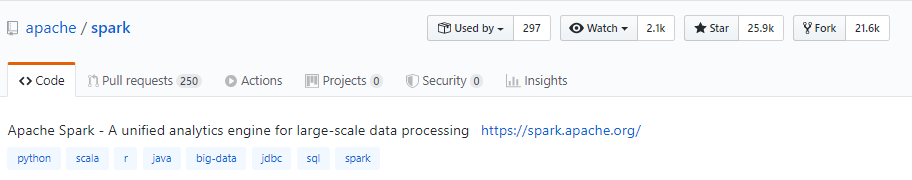
\includegraphics[width=0.8\linewidth]{figs/spark_topics.png}
	\caption{Example of a \GH repository and its topics.}
	\label{fig:spark}
\end{figure*}

As mentioned before, the \MNB using the \RM file of a repository to predict featured topics. It involves all the standard techniques employed in the ML domain \ie textual engineering, feature extraction, and training phase. By relying on the multinomial probability distribution, the approach is able to extract relevant information from the \RM file and suggest a set of topics. Table \ref{tab:example} shows an example of the \MNB's outcomes given the list of the actual repository topics. 

\begin{table}[h]
\centering

\resizebox{8.5cm}{!} {

\begin{tabular}{| p{3.2cm} | p{3.2cm} | }
\hline
 \textbf{Actual Topics} &\textbf{ Predicted topics} \\ \hline
     python,blender-scripts, spaceship, procedural-generation, game-development, 3d        &  
  shell, terminal, \textbf{3d},	opengl,	\textbf{python}        \\ \hline

\end{tabular}
}
\caption{Example of the \MNB outcomes.\JDR{change the table with apache/spark data}}
\label{tab:example}
\end{table} 


Even though the \MNB works in practice, it suffers from some limitations. First, the underlying model can recommend only featured topics that represent only a small set of all possible terms that can be restricted because of antonymous term(\eg programming languages).
In this way, the \MNB doesn't express all the concepts covered by a \GH repository. As shown in the table, only two of the predicted topics matched with the real ones. The second major limitation is the underlying structure needed for the training phase. To deliver relevant items, the \MNB requires a \emph{balanced} dataset, \ie each topic must have a similar number of  \RM files. This scenario is difficult to meet in reality as the topics' heterogeneity is extremely high. Furthermore, the \GH platform is regularly updated with new projects and, consequently, with new topics. Thus, the training phase must take place several times to avoid outdated recommendations. 






\section{Proposed approach}
\label{sec:ProposedApproach}
%({\bf C}ross Project {\bf R}elationships for Computing {\bf O}pen {\bf S}ource {\bf S}oftware {\bf Sim}ilarity). 

%====================================================================================================================================
%By recommender systems,
%As described in the formal definition of the recommendation problem, at the base of each RS there are three main essential elements which are: users, items and ratings. Usually such information are represented all together by means of a user-item ratings matrix. Such ratings matrix consists of a table where each row represents a user, each column represents a specific item, and each entry represents the rating given by the user to the particular item. Usually, such matrix results very sparse in practice because users rate only a small portion of items. Fig. 2 shows an example of user-item ratings matrix in a movie RS where users express their preferences to the items (movies) by using a five points rating scale. The items with a question mark (unknown rating) are unseen for the corresponding user \cite{DBLP:conf/rweb/NoiaO15}.
%. The three main components that make up a recommender systems are 
%\paragraph{\textbf{User-item matrix}}
%\begin{figure}[h!]
%	\begin{equation} \nonumber
%	\bordermatrix{~ & she & is & today & a & nice & city \cr	
%		d_{1} 		& 1 & 1 & 0 & 0 & 1 & 0 \cr 
%		d_{2} 		& 0 & 1 & 1 & 0 & 1 & 0 \cr  
%		d_{3} 		& 0 & 1 & 0 & 1 & 2 & 1 \cr }
%	\end{equation}
%	\caption{An example of a term-document matrix}
%	\label{fig:TDM}
%\end{figure}
%; \emph{lib$_6$=commons-io:commons-io}
%====================================================================================================================================
%as an engine to generate recommendations using similarity values as its inputs.
%Given a project pi, by using CrossSim, we get a ranked list of similar projects. n is the number of most similar projects that are selected for the recommendation task. All libraries used by the top-n projects are used to compute recommendations for project pi. Number of recommended libraries: k. The number of libraries that are recommended to a test project. There are two main components in \CR: Similarity Computation and Recommendation Engine.  To evaluate a recommender system, we should take both components into account.
%====================================================================================================================================
%====================Find references that mention the importance of similarity computation and collaborative filtering. 
% they can improve productivity
%. Similar to the concept of user-item matrix.
%Afterwards, it selects the libraries using recommendation algorithms.
%With \CR we aim at supporting open source software developers by providing them with meaningful recommendations. 
%Projects with similar functionalities include similar libraries. 
%However, in the context of library recommendation, we consider the relationships of inclusion of libraries in projects.
% and an analogous user-item matrix is built to represent this relationship
%Generally, 
%====================================================================================================================================
%-library inclusion matrix of the projects, occurrence of the libraries as follows. %It is able to suggest libraries to a developer. 
% Using this representation, it is possible to compute the missing ratings by exploiting from the relationships \cite{reference/ml/MelvilleS10}. %To determine what products a given customer might like, they look for other customers who have assigned similar ratings to a similar range of products, and extrapolate from there. 
%which allows developers to select third-party libraries. 
%\eg those that help developers approach the most suitable resources.
%\subsection{Overview} \label{sec:Overview}
%It provides a library recommendation functionality, which is meaningful to OSS developers since it 
%allows them to search for third-party libraries that may be useful for their current project. In 
%this section the \CR approach is presented. 
% and third-party libraries
% on which third-party libraries should be included
%With regards to the rich metadata infrastructure available at OSS repositories, we represent the cross relationships using the graph model, so as to compute similarities among various artifacts. 
% to support OSS developers
%====================================================================================================================================

In this section, we describe \CT that provides developers with relevant topics for \GH repositories. More specifically, \CT is a \emph{recommender system} \cite{Aggarwal2016} that encodes the relationships among different topics by means of a graph and utilizes a collaborative filtering technique \cite{Schafer:2007:CFR:1768197.1768208} to recommend \GH topics. Such a technique has been used mostly in the e-commerce domain to exploit the relationships among users and products to predict the missing ratings of recommended items \cite{Linden:2003:ARI:642462.642471}. The technique follows the assumption that \emph{``if users agree about the quality or relevance of some items, then they will likely agree about other items''} \cite{Schafer:2007:CFR:1768197.1768208}. Under the same premise, our tool aims to solve the problem of the reachability of a \GH repository given a set of topics. Instead of recommending goods or services to customers, we recommend a set of topics using an analogous mechanism: \emph{``if a user tags his project with some topics, then similar projects will probably contain common topics.''} 

\begin{figure}[t!]
	\centering
	\includegraphics[width=\linewidth]{figs/CFTop.pdf}
	\caption{Overview of the \CT Architecture.}% [??Rename Similarity Computation with Similarity Calculator]
	\label{fig:CrossRecArchitecture}
\end{figure}

%
To this end, the architecture of \CT is shown in Fig. \ref{fig:CrossRecArchitecture}, and consists of the software components supporting the following activities:

\begin{itemize}
\item \textit{Representing the relationships} among projects and topics retrieved from existing repositories;
\item \textit{Computing similarities} to find projects, which are similar to that under development; and
\item \textit{Recommending topics} to projects using a collaborative-filtering technique.
\end{itemize}


%\emph{mathematically computable format}

In a typical usage scenario of \CT, we assume that a developer is creating a new \GH repository, in which she has already included some topics to improve its reachability.
As shown in Fig. \ref{fig:CrossRecArchitecture}, the developer interacts with the system by demanding for recommendations.
Such a request contains a list of topics that are already included in the project the developer is working on. As a preprocessing phase, we apply a \emph{Topic filter} according to their frequencies \ie the measured occurrences over all repositories in the initial dataset. 
The \code{Graph Encoder} represents
the mentioned repositories in the graph format. This is a preparatory phase for the next steps of the recommendation process. The \code{Similarity Calculator} module computes similarities among topics to discover similar ones to recommend. The \code{Recommendation Engine} 
implements a \emph{collaborative-filtering} technique
\cite{Aggarwal2016},\cite{Zhao:2010:UCR:1748610.1749278}, it selects top-$k$ similar topics, and performs computation to generate a ranked list of \emph{top-N}
topics.~Finally, the final list of topics is sent back to the developer.

The aforementioned components are singularly described in the next sections.
 % shown in Fig. \ref{fig:CrossRecArchitecture} \cite{CROSSREC-DATA}

%\vspace{-.2cm}
%analyzes the input to 
%CrossRec represents the data collected from OSS repositories.
%. The data collected from OSS repositories is converted into a matrix 
%A matrix of this type is very sparse since most users give ratings to a small amount of items. 
\subsection{Topic filter}  \label{sec:filter}
As a preprocessing, we filter the initial set of topics using their frequencies counted on the entire \GH dataset. We remove irrelevant topics to reduce the noise in the prediction phase. Through the \emph{cut-off} value, we progressively increase the frequency threshold to evaluate possible impacts on overall performances. As stated in \cite{repo-topix}, this preprocessing can improve the final results, thus we decide to apply it as a first step. 



\subsection{Data Encoder} \label{sec:DataEncoder}

Considering traditional recommender systems for online services, we can identify three main components, namely \emph{users}, \emph{items}, and
\emph{ratings} \cite{Sarwar:2001:ICF:371920.372071},\cite{DBLP:conf/rweb/NoiaO15}. All mutual relationships among system components are encoded in a \emph{user-item ratings matrix}. Specifically, in the matrix a user is represented by a row,
an item is represented by a column and each cell in the matrix corresponds to a rating given by a user for an item
\cite{DBLP:conf/rweb/NoiaO15}. Moving to our domain, users are substitute by projects as well as topics are the possible items to recommend. The analogus user-item ratings matrix represents possible relationships between these two elements \ie project may include various topics. We can denote \emph{project-library inclusion} relationships as $\ni$. In this matrix, each row represents a project and each column represents a topic. A cell in the matrix is set to $1$ if the topic in the column is included in the project specified by the row, it is set to $0$
otherwise. For the sake of clarity and conformance, we still denote this as a user-item ratings matrix throughout this
paper.

For explanatory purposes, we consider a set of four projects $P=\{p_1,p_2,p_3,p_4 \}$ together with a set of topics $L=\{$\emph{topic$_1$=machine-learning}; \emph{topic$_2$=javascript}; topic{lib$_3$=database}; \emph{topic$_4$=web}; \emph{topic$_5$=al-gorithm}$\}$. By extracting the list of defined topics of the projects in $P$, we discovered the following inclusions: $p_1 \ni topic_1,topic_2$; $p_2 \ni topic_1,topic_3$; $p_3 \ni topic_1 ,topic_3, topic_4, topic_5$;\\
$p_4 \ni topic_1,topic_2,topic_4,topic_5$. Accordingly, the user-item ratings matrix built to model the occurrence of the topic is depicted in Fig.~\ref{fig:UserItemMatrix}.


%====================================================================================================================================
%\footnote{The file \emph{pom.xml} defines all project dependencies with external Maven libraries (\url{https://maven.apache.org/guides/introduction/introduction-to-the-pom.html}) }
%By performing an observation on a data set consisting of more than one thousand GitHub Java projects, we found out that the project-library inclusion matrix is very sparse since most projects contain a limited number of libraries, whereas the total number of libraries included by the projects is pretty large.

%There are two key components: Similarity Computation and Recommendation Engine. The Similarity computation module performs. Based on the list of libraries. Similarity computation is important.
%The former is used to compute similarity between different artifacts, \eg projects, libraries, or even developers. 
%====================================================================================================================================
%is of highly importance. The ability to find most similar projects 
%Similarity computation plays a key role in. Measuring the similarities between developers and software projects is a critical phase for most types of recommender systems \cite{DBLP:conf/rweb/NoiaO15}. Similarities are used as a base by both content-based and collaborative-filtering recommender systems to choose the most suitable and meaningful items for a given item \cite{Schafer:2007:CFR:1768197.1768208}. Failing to compute precise similarities means concurrently adding a decline in the overall performance of these systems. 
%====================================================================================================================================
%Using a recommendation algorithm, CrossRec selects the top most libraries as recommendations. The Recommendation Engine searches for libraries that are included in the similar projects. 
%We also investigate the effect of similarity computation by considering two similarity metrics. 
%Currently, CrossRec supports only GitHub, for future implementation, we expect to include various.
%To incorporate. Based on two premises: Projects use similar libraries to implement similar functionalities. And similar projects use similar set of libraries. To this end, we concentrate on finding a practical solution to represent the relationships between the artifacts, and eventually to compute similarity and cluster OSS projects.
%To compute the similarity between two open software projects. The graph representation allows for different similarity algorithms. In the scope of this paper, we choose the algorithm proposed by \emph{Di Noia et al.} for computing. For future work, other algorithms can also be flexibly included as long as they are suitable for graph.
%: either (i) there are direct links between them; or (ii)
%; or (iii) they are pointed by the same subject with the same property
%For library recommendation, we consider only one property, i.e. \emph{includes} (See Fig. \ref{fig:Graph}). 
%The similarity between $\alpha$ and $\beta$ 
%on a set of properties $P$ is the weighted mean of the values by all properties in $P$ as given below:  
%\begin{equation*}
%VsmSim(\alpha,\beta)=\frac{\sum_{p\in P} \omega_p VsmSim_{p}(\alpha,\beta)}{|P|}
%\end{equation*}
%to compute similarity and finally to provide inputs for a recommender system. 
%====================================================================================================================================
% makes, similarity computation becomes more complicated as many artifacts and several cross relationships prevail.
%As the input for the recommendation process, it is necessary to compute the similarity among software projects. 
%The ability of recommendation is important in the context of mining software repositories. 
%Understanding the similarity between software projects allows for reusing of codes and prototyping, or choosing alternative implementations \cite{10.1109/SANER.2017.7884605}. 
%We see that the ability to measure the similarity between artifacts, \eg projects, code snippets, or even developers, is of highly importance. Meanwhile measuring the similarity between developers and software projects is a critical phase for most types of recommender systems. 
%By considering the analogy of typical applications of RDF graphs and the problem of detecting the similarity of open source projects, in this section we propose. 
%to different open source software projects and 
%an approach that makes use of graphs for representing different kinds of relationships in the OSS ecosystem. 
%One of its applications is to compute similarity computation for supporting recommender systems \cite{DiNoia:2012:LOD:2362499.2362501}.
%With the adoption of the graph representation, it is possible to compute similarity among artifacts exploiting numerous number of graph similarity algorithms. 
%Based on the graph structure, one can exploit nodes, links and the mutual relationships to compute similarity using existing graph similarity algorithms. 
% are incorporated into the similarity calculation
% , given an input project \emph{p}, CrossRec searches for libraries by considering the most similar projects to \emph{p}. 
%====================================================================================================================================
%The rich metadata infrastructure available from the \projectName Knowledge Base is attributed to various artifacts, such as source code, API calls, forum discussions, and bug reports. 
%To this end, we concentrate on finding a practical solution to represent the relationships between the artifacts, and eventually to compute similarity and cluster OSS projects.
%We believe that a homogeneous and formal representation of the intrinsic features of OSS repositories is needed to effectively support project similarity computation.
%In this system, either humans or non-human factors have mutual dependency and implication on the others. 
%A directed graph is defined as a tuple $G=(V,E,R)$, with $V$ being the set of vertices, $E$ being the set of edges and $R$ representing the relationship among the nodes. 
% and Fig. \ref{fig:UserItemMatrix}. 
%sketches the graph representation .  the representation for 
%Specifically, the graph model has been chosen since it allows 
%\todo[size=\tiny, color=green!40]{Nr. 11}
%====================================================================================================================================




\subsection{Similarity Calculator} \label{sec:SimilarityCalculator}

%The \code{Recommendation Engine} of \CT works by relying on an analogous user-item ratings matrix. To provide 
%inputs for this module, the first task of \CT is to perform similarity computation on its input data to find the 
%most similar projects to a given project. In this respect, the ability to compute the similarities among projects has 
%an effect on the recommendation outcomes.~Nonetheless, computing similarities among software systems is considered to 
%be a difficult task \cite{McMillan:2012:DSS:2337223.2337267}. In addition, the diversity of artifacts in OSS 
%repositories as well as their cross relationship makes the similarity computation become even more complicated. In OSS 
%repositories, both humans (\ie developers and users) and non-human actors (such as repositories, and libraries) have 
%mutual dependency and implication on the others. The interactions among these components, such as developers commit to 
%or star repositories, or projects include libraries, create a tie between them and should be included in similarity 
%computation.
%
%%Furthermore, the graph structure also facilitates graph kernel methods, which are an effective way to compute similarities \cite{ODMD14a}. 
%%As being inspired by the research from the related Linked Data and Semantic Web field \cite{bizer_linked_2009}, 
%% as done \eg in ~\cite{Nguyen:2015:CRV:2942298.2942305,NDRDSEAA2018}
%% \hl{The representation is inspired by the one presented in}~\cite{NDRDSEAA2018}, however the relationship between projects and libraries is the inverse semantic path, i.e. \texttt{includes} instead of \texttt{isUsedBy}.
%
%
%We assume that a representation model that addresses the semantic 
%relationships among miscellaneous factors in the OSS community is beneficial to 
%project similarity computation. To this end, we consider the community of developers together with 
%OSS projects, topics, and their mutual interactions as an 
%\textit{ecosystem}. We derive a 
%\textit{graph-based} model to represent different kinds of relationships in the OSS ecosystem, and 
%eventually to calculate similarities. In the context of mining OSS repositories, the graph model is a convenient approach since it allows for flexible data integration and numerous computation techniques. 
%By applying this representation, we are able to transform the set of projects and topics shown in Fig.~\ref{fig:UserItemMatrix} into a directed graph as in Fig.~\ref{fig:Graph}.
%%\todo[size=\tiny, color=green!40]{This refers to our SEAA paper} 
%%In Linked Data, an RDF\footnote{RDF 1.1 Concepts and Abstract Syntax: \url{https://www.w3.org/TR/2014/REC-rdf11-concepts-20140225/}} graph is made up of an enormous number of nodes and oriented links with semantic relationships. Thanks to this feature, the similarity of two nodes in a graph can be computed by considering their intrinsic characteristics like neighbour nodes and their mutual interactions \cite{DiNoia:2012:LOD:2362499.2362501,Nguyen:2015:CRV:2942298.2942305}.
%~We adopted our proposed CrossSim approach~\cite{Nguyen:2019:FRS:3339505.3339636},\cite{8498236} to compute the 
%similarities among OSS graph nodes. It relies on techniques successfully 
%exploited by many studies to do the same task 
%\cite{DiNoia:2012:LOD:2362499.2362501},\cite{BRIGUEZ20146467}. Among 
%other relationships, two nodes are deemed to be similar if they point to the same node with the same edge. By looking at the graph in 
%Fig.~\ref{fig:Graph}, we can notice that $p_3$ and $p_4$ are highly 
%similar since they both point to three nodes $topic_{1}, topic_{4}, topic_{5}$.  This 
%reflects what also suggested in a previous work by McMillan \etal 
%\cite{McMillan:2012:DSS:2337223.2337267}, \ie similar projects implement common 
%pieces of functionality by using a shared set of libraries.
%
%
%\begin{figure}[t!]
%	\centering
%	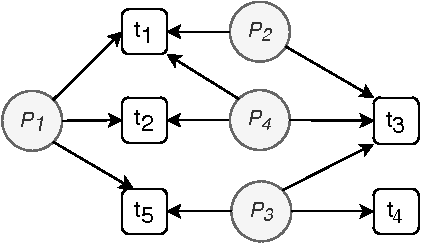
\includegraphics[width=\columnwidth]{figs/Graph.pdf}
%	\caption{Graph representation for projects and libraries.}
%	\label{fig:Graph}
%\end{figure}




The \code{Recommendation Engine} of \CT works by relying on the mentioned user-item ratings matrix. To provide
inputs for this module, the first task of \CT is to apply a similarity function on its input data to find the
most similar topics to a given initial set. Computing properly this similarity score affects the quality of recommendation outcomes.


~Nonetheless, computing similarities among topics could be a daunting task. \GH allows any repository owner to add, change, or delete the list of topics that describe his project \cite{}. This impacts on the stability of the topics, as they can change rapidly over time. In addition, a developer can freely specify the entire set of topics. This makes the similarity computation more complicated, as some topics couldn't have a semantic link with the others. Moreover, we can miss some key relationships depending on the similarity function employed by the calculator. For example, a purely sintactic-based similarity function assign a lower score to the topic pair 3d-graphics even though these two terms are strongly bounded in their meaning. 




We assume that a representation model that addresses mutual
relationships among \GH repositories and their topics is profitable to
proposed similarity computation. To this end, we derive a
\textit{graph-based} model to represent this kind of relationships and eventually to calculate similarities. In the context of mining OSS repositories, the graph model is a convenient approach since it allows for flexible data integration and numerous computation techniques.
By applying this representation, we are able to transform the set of projects and topics shown in Fig.~\ref{fig:UserItemMatrix} into a directed graph as in Fig.~\ref{fig:Graph}.
~We adopted our proposed CrossSim approach~\cite{Nguyen:2019:FRS:3339505.3339636},\cite{8498236} to compute the
similarities among OSS graph nodes. It relies on techniques successfully
exploited by many studies to do the same task
\cite{DiNoia:2012:LOD:2362499.2362501},\cite{BRIGUEZ20146467}. Among
other relationships, two nodes are deemed to be similar if they point to the same node with the same edge. By looking at the graph in
Fig.~\ref{fig:Graph}, we can notice that $p_3$ and $p_4$ are highly
similar since they both point to three nodes $topic_{1}, topic_{4}, topic_{5}$. This
reflects what also suggested in a previous work by McMillan \etal
\cite{McMillan:2012:DSS:2337223.2337267}, \ie similar projects implement common
pieces of functionality by using a shared set of libraries.


\begin{figure}[t!]
\centering
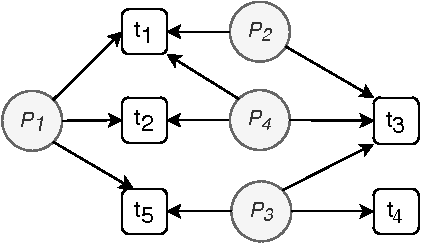
\includegraphics[width=\columnwidth]{figs/Graph.pdf}
\caption{Graph representation for projects and libraries.}
\label{fig:Graph}
\end{figure}


Using this metric, the similarity between two project nodes $p$ and $q$ in an OSS graph is computed 
by considering their feature sets \cite{DiNoia:2012:LOD:2362499.2362501}. Given that $p$ has a 
set of neighbor nodes 
$(topic_{1},topic_{2},..,topic_{l})$, the features of $p$ are represented by a vector 
$\overrightarrow{\phi}=(\phi_{1},\phi_{2},..,\phi_{l})$, with $\phi_{i}$ being the weight of node 
$topic_{i}$. It is computed as the \emph{term-frequency inverse document frequency} value as follows: 
%\texttt{tf-idf}   of the node 
%\vspace{-.1cm}
\begin{equation}\label{eqn:TFIDF}
\phi_{i} = f_{topic_{i}} \times log(\frac{ \left | P \right |}{a_{topic_{i}}})
\end{equation}

\noindent
where $f_{topic_{i}}$ is the number of occurrence of $topic_{i}$ with respect to $p$, it can be either $0$ and $1$ since there is a maximum of one $topic_{i}$ connected to $p$ by the edge \emph{includes}; $\left | P \right |$ is the total number of considered projects; $a_{topic_{i}}$ is the number of projects connecting to $topic_{i}$ via the edge \emph{includes}. %According to Eq.~\ref{eqn:TFIDF}, node $topic_{1}$ in Fig.~\ref{fig:Graph} has a low weight compared to that of other nodes since it is pointed by all four project nodes. In practice, this is comprehensible since \emph{junit:junit} is a very popular dependency and thus it should have a less important role in characterizing a project.
Eventually, the similarity between $p$ and $q$ with their corresponding feature vectors $\overrightarrow{\phi}=\{\phi_{i}\}_{i=1,..,l}$ and $\overrightarrow{\omega}=\{\omega_{j}\}_{j=1,..,m}$ is computed as given below:%\todo[size=\tiny, color=green!40]{Nr. 3}
%\vspace{-.2cm}

\begin{equation} \label{eqn:VsmSim}
sim(p,q)=\frac{\sum_{t=1}^{n}\phi_{t}\times \omega_{t}}{\sqrt{\sum_{t=1}^{n}(\phi_{t})^{2} }\times \sqrt{\sum_{t=1}^{n}(\omega_{t})^{2}}} 
\end{equation}

%\noindent
where $n$ is the cardinality of the set of topics that $p$ and $q$ share in common \cite{DiNoia:2012:LOD:2362499.2362501}. Intuitively, $p$ and $q$ are characterized by using vectors in an $n$-dimensional space, and Eq.~\ref{eqn:VsmSim} measures the cosine of the angle between the two vectors. %and it is computed using the inner product as follows.







%\textbf{??Intuitive description of eq 2 is needed.}
%====================================================================================================================================
%in which $\omega_p$ is the weight for property $p$ and computed using a genetic algorithm. 
%The hypothesis is based on the fact that the projects are aiming at creating common functionalities by using common libraries.
%In \cite{Jeh:2002:SMS:775047.775126}, SimRank has been developed to calculate similarities based on mutual relationships between graph nodes. Considering two nodes, the more similar nodes point to them, the more similar the two nodes are. In this sense, the similarity between two nodes $\alpha,\beta \in V$ is computed by using a fixed-point function. Given $k \geq 0$ we have $R^{(k)}(\alpha,\beta) = 1$ with $\alpha = \beta$ and $R^{(k)}(\alpha,\beta) = 0$ with $k=0$ and $\alpha \neq \beta$, SimRank is computed as follows:
%
%\begin{equation}\label{eqn:SimRank}
%R^{(k+1)}(\alpha,\beta) = 
%\frac{\Delta}{|I(\alpha)|\cdot|I(\beta)|}\sum_{i=1}^{|I(\alpha)|}\sum_{j=1}^{|I(\beta)|}R^{(k)}(I_{i}(\alpha),I_{j}(\beta))
%\end{equation}
%
%where $\Delta$ is a damping factor ($0 \leq \Delta < 1$); $I(\alpha)$ and $I(\beta)$ are the set of incoming neighbors of $\alpha$ and $\beta$, respectively. $|I(\alpha)|\cdot|I(\beta)|$ is the factor used to normalize the sum, thus forcing $R^{(k)}(\alpha,\beta) \in [0,1]$. 
%
%For the first implementation of CrossSim we adopt SimRank as the mechanism for computing similarities among OSS graph nodes. For future work, other similarity algorithms can also be flexibly integrated into CrossSim, as long as they are designed for graph. %as long as. is able to incorporate various similarity algorithms, 
%\begin{figure}[t!]
%	\centering
%	\includegraphics[width=0.3\textwidth]{figs/SimRank.pdf}
%	\caption{SimRank similarity}
%	\label{fig:SimRank}
%\end{figure}
%====================================================================================================================================
%Equation~\ref{eqn:SimRank} implies that the similarity for two nodes is computed by aggregating the similarity of all possible pairs of their neighbors. 
%We are convinced that the utilization of SimRank is convenient and practical also when various relationships are incorporated into the graph. Given the circumstances, the algorithm needs not be changed since it only works on the basis of nodes and edges. In this sense, 
% \emph{CrossSim} is a versatile similarity tool as it can accept various input features regardless of their format. 
%To study the performance of CrossSim we conducted a comprehensive evaluation using a real dataset collected from GitHub. To aim for an unbiased comparison, we opted for existing evaluation methodologies from other studies of the same type \cite{Lo:2012:DSA:2473496.2473616,McMillan:2012:DSS:2337223.2337267,10.1109/SANER.2017.7884605}. Together with other metrics typically used for evaluations, i.e. \textit{Success rate}, \textit{Confidence},  \textit{Number of false positives}, and \textit{Precision}, we decided to use also \textit{Ranking} to measure the sensitivity of the similarity tools to ranking results. The details of our evaluation are given in the next section. In the first place, it is necessary to compute similarities among projects.
%In this case, the ratings provided by similar users to a target user A are used to make recommendations for A. %The predicted ratings of A are computed as the weighted average values of these “peer group” ratings for each item. 
%From: https://www.sciencedaily.com/releases/2017/12/171206122420.htm
%The recommendation systems at websites such as Amazon and Netflix use a technique called "collaborative filtering."
%To compute the missing ratings, generally there are two ways corresponding to the way we exploit the user-item matrix. In this paper, we investigate both types of collaborative-filtering recommender system: user-based and item-based.
%\paragraph{\textbf{User-based collaborative filtering}}
%One of the most promising such technologies is collaborative filtering [19, 27, 14, 16]. 
%works by filtering or evaluating items using the preferences of other users. 
%In this approach personalized recommendations for a target user are generated using opinions of users having similar tastes to those of the target user. The main assumption in this approach is that users with similar preferences in the past will have similar preferences in the future.
% To compute the missing ratings, there are two main ways, which are basically based on the column-wise and row-wise relationships of the user-item ratings matrix. For \emph{user-based collaborative filtering}. Exploit the relationships among users to deduce the missing ratings. 
%The missing ratings for a given user are computed by exploiting the existing ratings from other similar users. Row-wise computation, among the top most similar projects. 
%====================================================================================================================================
%By online systems, collaborative filtering works by searching for similar. by building a database of preferences for items by users. A new user, Neo, is matched against the database to discover neighbors, which are other users who have historically had similar taste to Neo. Items that the neighbors like are then recommended to Neo, as he will probably also like them. Collaborative filtering has been very successful in both research and practice, and in both information filtering applications and E-commerce applications. However, there remain important research questions in overcoming two fundamental challenges for collaborative filtering recommender systems (Item-based Collaborative Filtering Recommendation Algorithms).
%In addition, collaborative-filtering is considered to be better. 
%from these. calculates similarity between users by comparing their ratings on the same item, and it then computes the predicted rating for an item by the active user
%similar to the active user where weights are the similarities of these users with the target item
%(i.e. the user requiring a prediction) 
%====================================================================================================================================

%A collaborative-filtering recommender system suggests products that customers similar to the customer being considered have already purchased. 


The representation using a user-item ratings matrix allows for the computation of missing scores \cite{Aggarwal2016},\cite{DBLP:conf/rweb/NoiaO15}. Depending on the availability of data, there are two main techniques to compute the unknown ratings, namely \emph{content-based} \cite{Pazzani2007} and \emph{collaborative-filtering} \cite{Miranda:2008:ICF:1486927.1487083} recommendation techniques. Focusing on the latter, this technique computes the ratings by taking into account the set of items rated by similar customers. There are two main types of collaborative-filtering recommendation: \emph{user-based} \cite{Zhao:2010:UCR:1748610.1749278} and \emph{item-based} \cite{Sarwar:2001:ICF:371920.372071} techniques. As their names suggest, the user-based technique computes missing ratings by considering the ratings collected from similar users. Instead, the item-based technique performs the same task by using the similarities among items \cite{Cremonesi:2008:EMC:1468165.1468327}.

In the context of \CT, the term \emph{rating} describes the appearance of a topic in a project and the employed collaborative filtering techniques aim to find additional similar topics. The project that needs prediction for topic suggestion is called the \emph{active project}. By the matrix in Fig. \ref{fig:UserBasedCF}, $p$ is the active project and an asterisk ($*$) represents a known rating, either $0$ or $1$, whereas a question mark ($?$) represents an unknown rating and needs to be predicted.



\begin{figure}[t!]
\centering
%	\vspace{-.4cm}
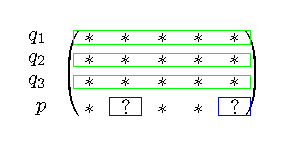
\includegraphics[width=0.7\linewidth]{figs/UserBasedCF.pdf}
\vspace{-.4cm}
\caption{Computation of missing ratings using the user-based collaborative-filtering technique~\cite{Zhao:2010:UCR:1748610.1749278}.}% [?? In the previous version there was a rectangle including some of the rows. Isn't?]
\vspace{-.1cm}
\label{fig:UserBasedCF}
\end{figure}


Consider the mutual relationships between a project and its topics represented in a graph data structure, we exploit the user-based collaborative-filtering technique to enable the topic recommendation process \cite{Linden:2003:ARI:642462.642471,Zhao:2010:UCR:1748610.1749278}. Given an active project $p$, the inclusion of libraries in $p$ can be deduced from projects that are similar to $p$. The process is summarized as follows: 

\begin{itemize}
\item Compute the similarities between the active project and all projects in the collection;
\item Select \emph{top-k} most similar projects; and %a subset of the users (neighborhood) according to their similarity with the active user;
\item Predict ratings by means of those collected from the most similar projects.
\end{itemize}

The rectangles in Fig. \ref{fig:UserBasedCF} imply that the row-wise relationships between the active project $p$ and the similar projects $q_1,q_2,q_3$ are exploited to compute the missing ratings for $p$. The following formula is used to predict if $p$ should include $l$, \ie~$p \ni l$~\cite{DBLP:conf/rweb/NoiaO15}: % the predicted value $r_{p,l}$ is computed
%\vspace{-.2cm}
\begin{equation} \label{eqn:Prediction}
r_{p,l}=\overline{r_{p}}+\frac{\sum_{q \in topsim(p)}(r_{q,l}-\overline{r_{q}})\cdot sim(p,q) }{\sum_{q \in topsim(p)} sim(p,q) } %\left | P \right |
\end{equation}

\noindent
where $\overline{r_{p}}$ and $\overline{r_{q}}$ are the mean of the ratings of $p$ and $q$, respectively; $q$ belongs to the set of \emph{top-k} most similar projects to $p$, denoted as $topsim(p)$; $sim(p,q)$ is the similarity between the active project and a similar project $q$, and it is computed using Equation \ref{eqn:VsmSim}. %For a testing project $p$, $\overline{r_{p}}$ is equal to $1$ since the ratings for all testing libraries are $1$.




%\subsection{Recommendation Engine} \label{sec:RecommendationEngine}
%\PN{Please reprhare this section}
%The representation using a user-item ratings matrix allows for the computation of missing ratings \cite{Aggarwal2016},\cite{DBLP:conf/rweb/NoiaO15}. Depending on the availability of data, there are two main ways to compute the unknown ratings, namely \emph{content-based} \cite{Pazzani2007} and \emph{collaborative-filtering} \cite{Miranda:2008:ICF:1486927.1487083} recommendation techniques. The former exploits the relationships among items to predict the most similar items. The latter computes the ratings by taking into account the set of items rated by similar customers. There are two main types of collaborative-filtering recommendation: \emph{user-based} \cite{Zhao:2010:UCR:1748610.1749278} and \emph{item-based} \cite{Sarwar:2001:ICF:371920.372071} techniques. As their names suggest, the user-based technique computes missing ratings by considering the ratings collected from similar users. Instead, the item-based technique performs the same task by using the similarities among items \cite{Cremonesi:2008:EMC:1468165.1468327}.
%
%In the context of \CR, the term \emph{rating} is understood as the occurrence of a library in a project and computing missing ratings means to predict the inclusion of additional libraries. The project that needs prediction for library inclusion is called the \emph{active project}. By the matrix in Fig. \ref{fig:UserBasedCF}, $p$ is the active project and an asterisk ($*$) represents a known rating, either $0$ or $1$, whereas a question mark ($?$) represents an unknown rating and needs to be predicted.
%
%%Because of the above assumptions, the collaborative filtering algorithm is based on the comparison of one user’s behavior with other user’s behavior, to find his nearest neighbors, and according to his neighbor’s interests or preferences to predict his interests or preferences.
%
%\begin{figure}[t!]
%	\centering
%	%	\vspace{-.4cm}
%	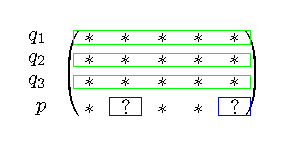
\includegraphics[width=0.7\linewidth]{figs/UserBasedCF.pdf}
%	\vspace{-.4cm}
%	\caption{Computation of missing ratings using the user-based collaborative-filtering technique~\cite{Zhao:2010:UCR:1748610.1749278}.}% [?? In the previous version there was a rectangle including some of the rows. Isn't?]
%	\vspace{-.1cm}
%	\label{fig:UserBasedCF}
%\end{figure}
%
%%\CR employs a collaborative-filtering technique   based on the similar model applied in e-commerce systems
%
%Given the availability of the cross-relationships as well as the possibility to compute similarities among projects using the graph representation, we exploit the user-based collaborative-filtering technique as the engine for recommendation \cite{Linden:2003:ARI:642462.642471,Zhao:2010:UCR:1748610.1749278}. Given an active project $p$, the inclusion of libraries in $p$ can be deduced from projects that are similar to $p$. The process is summarized as follows: % \cite{Cacheda:2011:CCF:1921591.1921593}:
%%In particular, the user-based collaborative-filtering technique predicts a missing rating by considering the most similar projects to $p$. 
%
%%%The engine first searches for similar projects and then computes missing ratings as a weighted average of the ratings of the items by projects .
%%According to [16, 15], item-based CF algorithms provide better performance and quality than user-based ones. Afterwards the unknown ratings are computed by considering the libraries included in these projects. In this paper, the user-based technique is utilized. 
%
%\begin{itemize} 	
%	\item Compute the similarities between the active project and all projects in the collection;
%	\item Select \emph{top-k} most similar projects; and %a subset of the users (neighborhood) according to their similarity with the active user;
%	\item Predict ratings by means of those collected from the most similar projects.
%\end{itemize} 
%
%The rectangles in Fig. \ref{fig:UserBasedCF} imply that the row-wise relationships between the active project $p$ and the similar projects $q_1,q_2,q_3$ are exploited to compute the missing ratings for $p$. The following formula is used to predict if $p$ should include $l$, \ie~$p \ni l$~\cite{DBLP:conf/rweb/NoiaO15}: % the predicted value $r_{p,l}$ is computed
%%\vspace{-.2cm}
%\begin{equation} \label{eqn:Prediction}
%r_{p,l}=\overline{r_{p}}+\frac{\sum_{q \in topsim(p)}(r_{q,l}-\overline{r_{q}})\cdot sim(p,q) }{\sum_{q \in topsim(p)} sim(p,q) }  %\left |  P \right |  
%\end{equation}
%
%\noindent
%where $\overline{r_{p}}$ and $\overline{r_{q}}$ are the mean of the ratings of $p$ and $q$, respectively; $q$ belongs to the set of \emph{top-k} most similar projects to $p$, denoted as $topsim(p)$; $sim(p,q)$ is the similarity between the active project and a similar project $q$, and it is computed using Equation \ref{eqn:VsmSim}. %For a testing project $p$, $\overline{r_{p}}$ is equal to $1$ since the ratings for all testing libraries are $1$. 


%\subsection{CrossRec in Action}
%\label{sec:inaction}
%In the context of the EU H2020 CROSSMINER project\footnote{\url{https://www.crossminer.org}}, we integrated \CR 
%into Eclipse as shown in Fig.~\ref{fig:IDE}. 
%The figure describes a development of an explanatory scenario where a 
%	developer is improving a software project, named \textit{aethereal} hereafter, 
%	by replacing some existing source code with features provided by third-party 
%	libraries. The goal of such changes is to make the code easier to be understood 
%	and evolved. The project is a command line tool written in Java that aims at 
%	supporting the automatic generation of cross-projects migration dependencies 
%	graph. To this aim \textit{aethereal} distinguishes between clients and 
%	libraries: both clients and libraries are Maven artifacts, and clients are 
%	defined as artifacts that use a specific  library available on the Maven 
%	repository.
%
%We explain how \CR helps the developer evolve the  \code{build} method of the class \code{MavenDataset} as follows.
%	Such a  method computes a dependency matrix between client versions and libraries. The initial implementation of the \code{build} method prints the logging information to the console by using Java I/O facilities (\ie~\code{System.out.println} and \code{System.err.println}) \circled{1}.
%	The \CR tool displays the list of third-party libraries currently being included \circled{2}, and prompts a list of recommended libraries \circled{3}. The list of recommended libraries highlights the suggestion for using a logging library, \ie~\code{slf4j}\footnote{\url{https://www.slf4j.org/}} or \code{{commons-logging}\footnote{\url{https://commons.apache.org/proper/commons-logging/}}}. Then, a possible migration to \code{slf4j} is shown \circled{4}, where the \code{System.out.println} and \code{System.err.println} invocations are replaced by \code{slf4j} \code{logger.info} and \code{logger.debug} calls, respectively.
%
%\begin{figure}[t!]
%	\centering
%	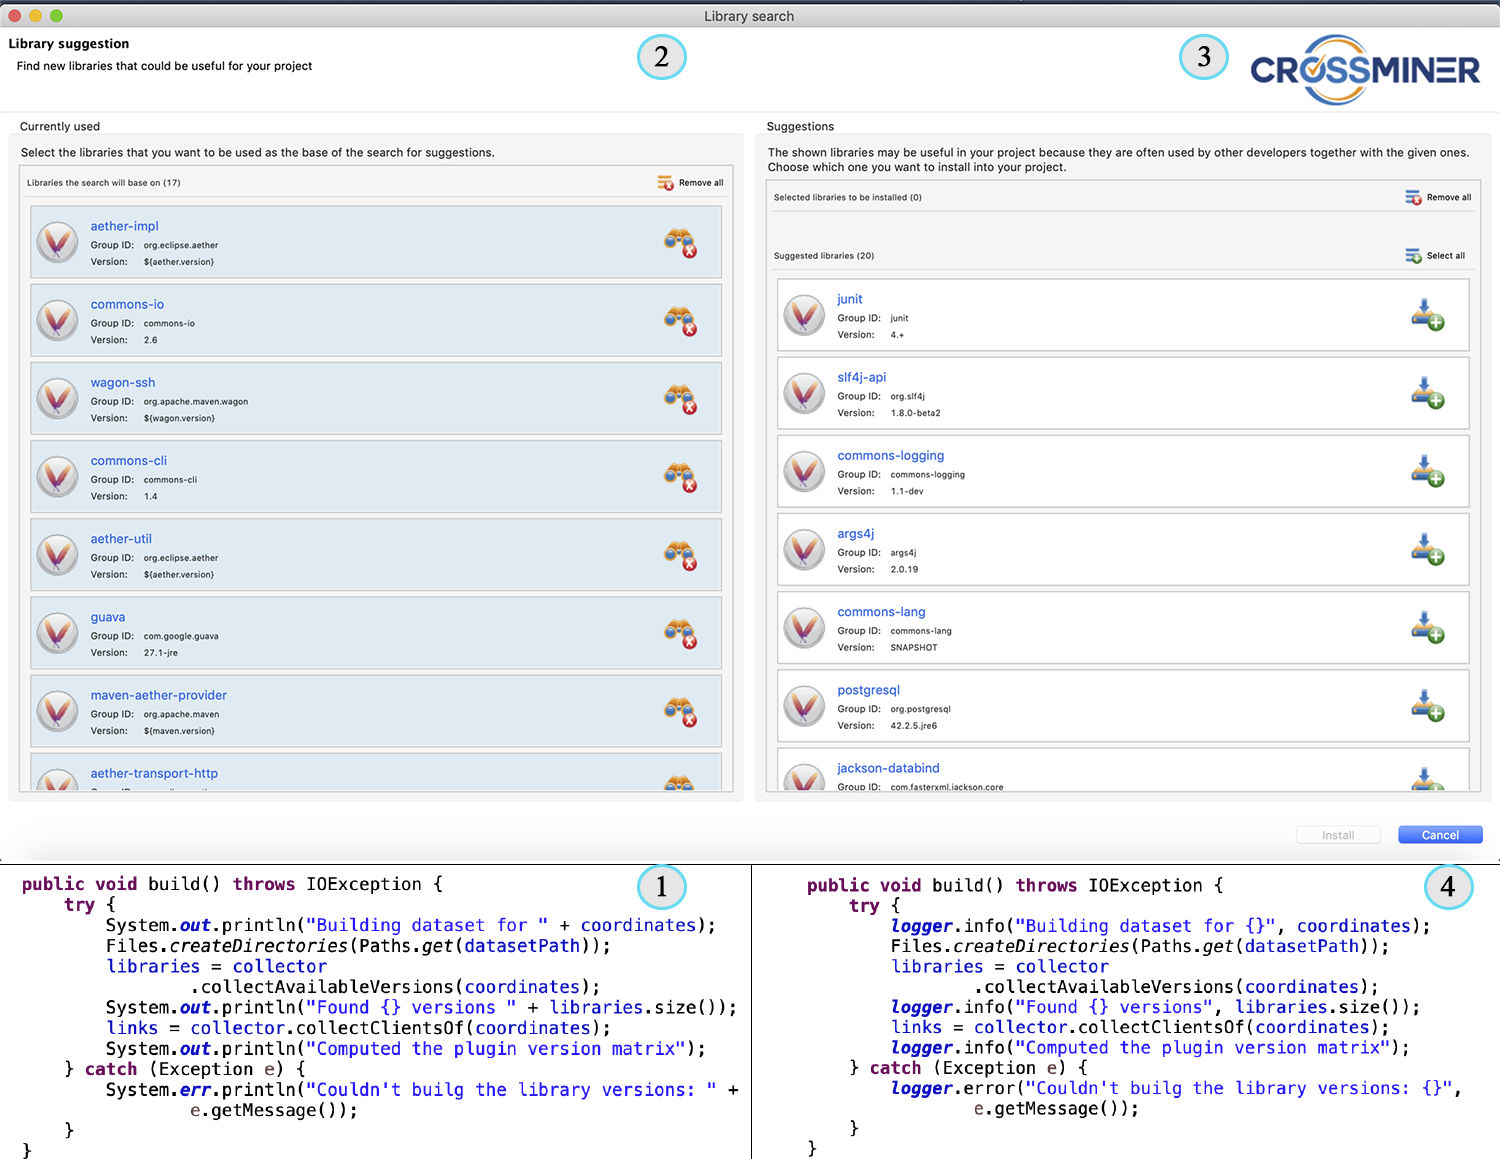
\includegraphics[wid\\th=\textwidth]{figs/CrossRecIDE.png}
%	%\vspace{-.3cm}
%	\caption{\CR IDE.}
%	\label{fig:IDE}
%	\vspace{-.3cm}
%\end{figure}
%
%
%
%In its current version, \CR recommends a set of libraries to developers, however it is likely that only some of the suggestions will result as useful for them. While the current version of \CR is unable to capture developers' feedback, it is possible to re-train again and obtain new recommendations based on the up-to-date code base.



\section{Evaluation Materials and Methods}		
\label{sec:Evaluation}
%In the following, we 

%\color{blue}




%\revised{:q

In this section, we report how \CT has been evaluated, having the {\em goal} of evaluating the performance of the proposed approach. In Section~\ref{sec:Dataset}, the dataset involved in our evaluation has been presented. We describe the evaluation methodology and metrics in Section~\ref{sec:methodology-metric}. Finally, Section~\ref{sec:ResearchQuestions} describes the research questions.


%ten equal parts, so-called folds
%We also exploited 
%was also exploited 

\begin{figure*}[h!]
	\centering
	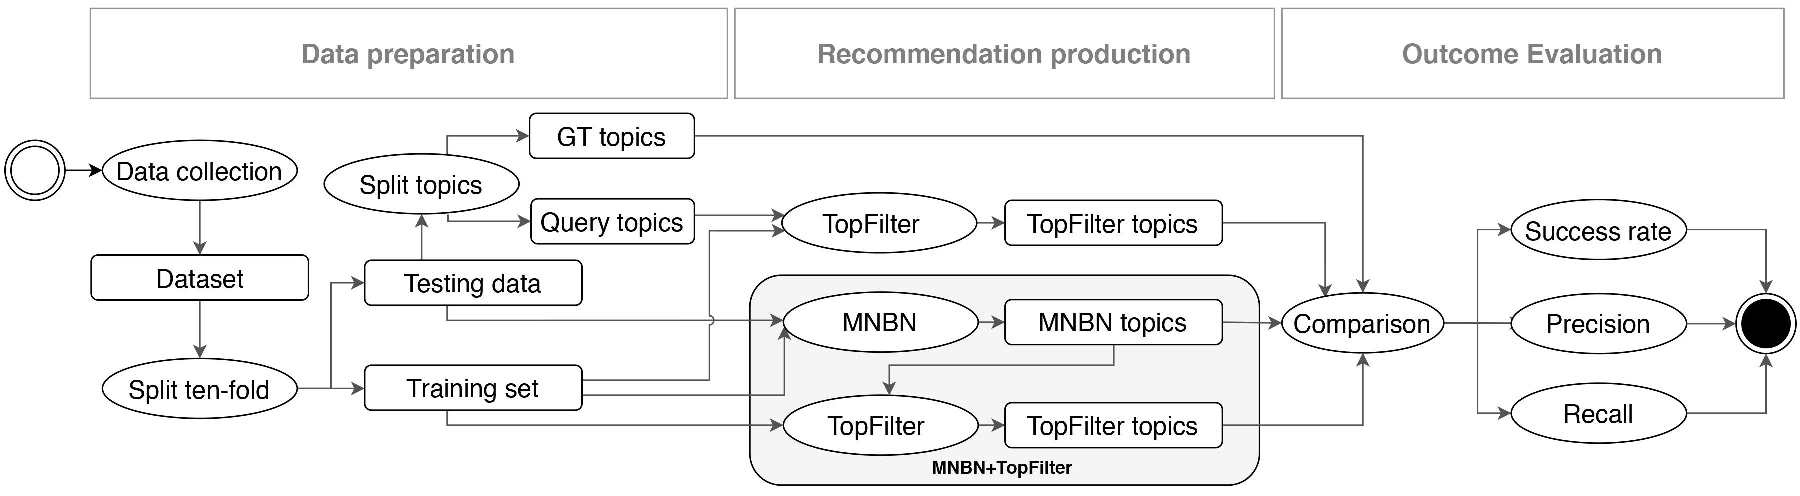
\includegraphics[width=0.9\linewidth,keepaspectratio]{figs/evaluationCF.pdf}
	%\vspace{-.3cm}
	\caption{Evaluation Process.}
	\label{fig:EvaluationProcess}
	\vspace{-.3cm}
\end{figure*}

\subsection{Dataset Extraction} \label{sec:Dataset}


%\color{blue}

To evaluate the approach, we reuse the same dataset employed for the \MNB available here \cite{MNBreplication}. The \GH query language \cite{understanding} allows the fetching of relevant repository metadata including name, owner, and list of topics to mention a few. Thus, we \emph{randomly} collected a dataset consisting of $6,258$ repositories that use 15757 topics by means of the GitHub API \cite{pygithub/pygithub_2019}. To overcome the request limit during the crawling activity, we employ the \GH star voting mechanism as a popularity measure \cite{borges_whats_2018}. As claimed in several works\cite{borges_popularity_2017, borges_predicting_2016}, a high number of stars means the attention of the community for that project. So, we impose the following filter during the query execution:
\begin{equation}
\small
Qf = "is:featured \; topic:t \; stars:100..80000 \; topics:>=2"
\end{equation}%
to consider only \GH repositories having a number of stars between 100 and 80,000, and tagged with at least two topics. The boolean qualifier \emph{is:featured} is used in the \MNB work to group repositories given a certain featured topic. As \CT is able to retrieve both featured and not-featured topics, this filter doesn't affect the quality of the collected data.




%Among these projects, only $7$ of them have been forked from other projects. Such original projects have been excluded from the dataset as their forked ones share highly similar libraries, and this may introduce bias in the recommendation outcomes. We represent the distribution of projects with respect to the number of forks, commits and pull requests in Fig.~\ref{fig:ForkCommitPull}. Most projects have a low number of pull requests, \ie lower than 100, however many of them have a large number of forks and commits. Forking is a means to contribute to the original repositories~\cite{Jiang:2017:WDF:3042021.3042043}. Furthermore, there is a strong correlation between forks and stars~\cite{7816479}, as it is further witnessed in Fig.~\ref{fig:ForkStarIssue}. A project with a high number of forks means that it gets attention from the OSS community. In this sense, having many forks can be considered as a sign of a well-maintained and well-received project. Meanwhile, as commits have an impact on the source code~\cite{8009930}, the number of commits is also a good indicator of how a project has been developed.
%}


%e mined dependency specification by means of \code{code.xml} or \code{.grad\-le} files.\footnote{The files \code{pom.xml} and with the extension \code{.gradle} are related to management of dependencies by means of Maven (\url{https://maven.apache.org/}) and Gradle (\url{https://gradle.org/}), respectively.} Fig.~\ref{fig:NumOfLibsD1} depicts the distribution of libraries across the projects. Most of the libraries in \code{D1} ($12,962$) are used by a small number of projects, and only $10$ libraries are extremely popular by being included in more than $200$ projects. By carefully investigating the dataset, we also see that most projects contain a small number of dependencies, \ie $48\%$ of the projects include less than $20$ libraries and just $15\%$ of them include more than $100$ libraries. \}


%\color{blue}
\subsection{Evaluation methodology and Metrics’ Definition}\label{sec:methodology-metric}

Figure~\ref{fig:EvaluationProcess} depicts the evaluation process consists of three consecutive phases,~\ie~\emph{Data Preparation},~\emph{Recommendation}, and~\emph{Outcome Evaluation}. \emph{Data Preparation} phase collects repositories that match the requirements defined in previous section from GitHub. This dataset is used to evaluate \CT, \MNB, and the combination of two. 
The dataset is then split into training and testing sets. The 
\emph{Recommendation} phase follows three different flows, according to the required input and produced output of the three mentioned approaches. In particular, the common operations are in white while the three different evaluation flows are represented in a grayscale fashion (\ie light grey, grey and dark grey boxes are related to \CT, \MNB, and entangled approaches evaluation respectively).
To enable \CT, we extract a portion of topics from a given testing project \ie the ground-truth part (it is defined as $GT(p)$ in the following). The left part is used as a query to produce recommendations (see the dotted line flow). As the \MNB uses the README file of a repository to predict a set of topics, this doesn't require any topic as input. Thus, the approach encodes the document relevant information in vectors using the TF-IDF weighting scheme. Then, to feed the network that delivers a set of topics (see the bold line). Finally, the entangled approach uses \CT as the recommendation engine which is fed by the \MNB suggested topics (see dashed line flow). All the results are assessed in the \emph{Outcome Evaluation} phase, which compares the recommendation results with those stored as ground-truth data to compute the quality metrics. 


The \emph{ten-fold cross-validation} methodology~\cite{kohavi1995study} has been used to assess the performance of \CT, \MNB and combined approach where every time $9$ folds 
%(each one contains $625$ projects) 
are used for training and the remaining one for testing.
For each testing project \emph{p}, we randomly delete half topics and save it as ground truth (\emph{GT(p)}) . The ground truth data  will be used to validate the recommendation outcomes. The remaining half topics are used as query topics to the \CT.%, which are called \emph{\textbf{te}}, and serve as input for \code{Similarity Computation} and \code{Recommendation} components.

The \code{Split topic phase} resembles a real development process where a developer has already included some topics in his repository and waits for recommendations \ie additional topics to be incorporated. \CT recommender system is expected to provide her with the other half, \ie \emph{GT(p)}. 

\JDR{Rephrase}There are several metrics available to evaluate a ranked list of recommended items \cite{DBLP:conf/rweb/NoiaO15}. In the scope of this paper, \emph{success rate} and \emph{accuracy} have been used to study the systems' performance as already proposed by Robillard \etal~\cite{Robillard:2014:RSS:2631387} and other studies~\cite{6671293},\cite{Nguyen:2015:ESP:2740908.2742141}. The metrics considered during the outcome evaluation follows this notation:

\begin{itemize}[noitemsep,topsep=0pt]
	\item \emph{t} is the frequency cut-off value of input topics (\ie all topics that occur less than \emph{t} times are removed from the dataset)
	\item \emph{N} is the cut-off value for the recommended ranked list of topic;% of recommended libraries;
	\item \emph{k} is the number of neighbor projects exploited for the recommendation process;
	\item For a testing project \emph{p}, a half of its topics are extracted and used as the ground-truth data named as \emph{GT(p)};
	\item $REC(p)$ is the \emph{top-N} topics recommended to \emph{p}. It is a ranked list in descending order of real scores;
	\item If a recommended topic $t \in REC(p)$ for a testing project $p$ is found in the ground truth of $p$ (\ie \emph{GT(p)}), hereafter we call this as a topic \textit{match}
\end{itemize}



If $REC_{N}(p)$ is the set of top-$N$ items and $match_{N}(p)$ is the set of items in the \emph{top-N} list that match with those in the ground-truth data, then the metrics are defined as follows.  

\vspace{.1cm}
\paragraph{\textbf{Success rate@N}} Given a set of testing projects \emph{P}, this metric measures the rate at which a recommender system returns at least a topic match among \emph{top-N} items for every project $p \in P$ \cite{6671293}: %It is formally defined as given below:
\vspace{-.1cm}

\begin{equation} \label{eqn:RecallRate}
success\ rate@N=\frac{ count_{p \in P}( \left | match_{N}(p) \right | > 0 ) }{\left | P \right |} %\times 100\%
%success\ rate@N=\frac{ count_{p \in P}( \left | GT(p) \bigcap (\cup_{r=1}^{N} REC_{r}(p)) \right | > 0 ) }{\left | P \right |}
\end{equation}

\vspace{.1cm}
\vspace{.1cm}
\paragraph{\textbf{Success rate$_M$@N}} Given a set of testing projects \emph{P}, this metric measures the rate at which a recommender system returns at least $M$ topics match among \emph{top-N} items for every project $p \in P$ \cite{6671293}: %It is formally defined as given below:
\vspace{-.1cm}

\begin{equation} \label{eqn:RecallRate}
success\ rate_M@N=\frac{ count_{p \in P}( \left | match_{N}(p) \right | >= M ) }{\left | P \right |} %\times 100\%
%success\ rate@N=\frac{ count_{p \in P}( \left | GT(p) \bigcap (\cup_{r=1}^{N} REC_{r}(p)) \right | > 0 ) }{\left | P \right |}
\end{equation}

\vspace{.1cm}
\noindent where the function \emph{count()} counts the number of times that the boolean expression specified in its parameter is \emph{true}.


\paragraph{\textbf{Accuracy}} Accuracy is considered as one of the most preferred \emph{quality indicators} for Information Retrieval applications \cite{Saracevic:1995:EEI:215206.215351}. However, \emph{success rate@N} does not reflect how accurate the outcome of a recommender system is. For instance, given only one testing project, there is no difference between a system that returns $1$ topic match out of $5$ and another system that returns all $5$ topic matches, since \emph{success rate@5} is $100\%$ for both cases (see Eq.~\eqref{eqn:RecallRate}). Thus, given a list of \emph{top-N} libraries, \emph{precision@N} and \emph{recall@N} are utilized to measure the \emph{accuracy} of the recommendation results. \emph{precision@N} is the ratio of the \emph{top-N} recommended topics belonging to the ground-truth dataset, whereas \emph{recall@N} is the ratio of the ground-truth topics appearing in the \emph{N} recommended items \cite{Nguyen:2019:FRS:3339505.3339636},\cite{DiNoia:2012:LOD:2362499.2362501},\cite{Davis:2006:RPR:1143844.1143874}: %,Nguyen:2015:CRV:2942298.2942305 %}. A concrete definition for the metrics is given below \cite{

%\vspace{-.2cm}
% \cite{Saracevic:1995:EEI:215206.215351}

\begin{equation} \label{eqn:Precision}
precision@N = \frac{ \left | match_{N}(p) \right | }{N}
%precision@N(p) = \frac{\sum_{r=1}^{N}\left | GT(p) \bigcap REC_{r}(p) \right |}{N}
\end{equation}
%\vspace{-.1cm}
\begin{equation} \label{eqn:Recall}
recall@N = \frac{ \left | match_{N}(p) \right | }{\left | GT(p) \right |}
%recall@N(p) = \frac{\sum_{r=1}^{N}\left | GT(p) \bigcap REC_{r}(p) \right |}{\left | GT(p) \right |}
\end{equation}
%\vspace{-.1cm}









%To assess the performance of \CR proposed approach, we applied ten-fold cross-validation, considering every time $9$ folds (each one contains $625$ projects) for training and the remaining one for testing. 
%	For every testing project \emph{p}, a half of its topics are \emph{randomly} 
%	taken out and saved as ground truth data, let us call them \emph{GT(p)}, which will be used to validate the recommendation outcomes. The other half are used 
%	as testing libraries or query, which are called \emph{\textbf{te}}, and serve 
%	as input for \code{Similarity Computation} and \code{Recommendation}.
%The splitting mimics a real development process where a 
%developer has already included some topics in the current project, \ie 
%\emph{\textbf{te}} and waits for recommendations, that means additional topics to be incorporated. A recommender system is expected to provide her 
%with the other half, \ie \emph{GT(p)}. %To ensure a reliable comparison between \LR and \CR, we performed cross-validation for both using exactly the same folds.
%
%
%
%There are several metrics available to evaluate a ranked list of recommended items \cite{DBLP:conf/rweb/NoiaO15}. In the scope of this paper, \emph{success rate}, \emph{accuracy}, \emph{sales diversity}, and \emph{novelty} have been used to study the systems' performance as already proposed by Robillard \etal~\cite{Robillard:2014:RSS:2631387} and other studies~\cite{6671293},\cite{Nguyen:2015:ESP:2740908.2742141}. For a clear presentation of the metrics considered during the outcome evaluation, let us introduce the following notations:
%
%\begin{itemize}[noitemsep,topsep=0pt]
%	\item \emph{N} is the cut-off value for the ranked list;% of recommended libraries;
%	\item \emph{k} is the number of neighbor projects exploited for the recommendation process;
%	\item For a testing project \emph{p}, a half of its libraries are extracted and used as the ground-truth data named as \emph{GT(p)};
%	\item $REC(p)$ is the \emph{top-N} libraries recommended to \emph{p}. It is a ranked list in descending order of real scores;%, with $REC_r(p)$ being the recommended library in the position $r$.		
%	\item If a recommended library $l \in REC(p)$ for a testing project $p$ is found in the ground truth of $p$ (\ie \emph{GT(p)}), hereafter we call this as a library \textit{match} or \textit{hit}.	
%\end{itemize}	
%
%
%
%If $REC_{N}(p)$ is the set of top-$N$ items and $match_{N}(p)=  GT(p) \bigcap REC_{N}(p) $ is the set of items in the \emph{top-N} list that match with those in the ground-truth data, then the metrics are defined as follows.
%
%\paragraph{\textbf{Success rate@N}} Given a set of testing projects \emph{P}, this metric measures the rate at which a recommender system returns at least a topic match among \emph{top-N} items for every project $p \in P$ \cite{6671293}: %It is formally defined as given below:
%\vspace{-.3cm}
%
%\begin{equation} \label{eqn:RecallRate}
%success\ rate@N=\frac{ count_{p \in P}( \left |  match_{N}(p) \right | > 0 ) }{\left | P \right |} %\times 100\%
%%success\ rate@N=\frac{ count_{p \in P}( \left |  GT(p) \bigcap (\cup_{r=1}^{N} REC_{r}(p)) \right | > 0 ) }{\left | P \right |} 
%\end{equation}
%
%\noindent where the function \emph{count()} counts the number of times that the boolean expression specified in its parameter is \emph{true}.
%
%
%\paragraph{\textbf{Accuracy}} Accuracy is considered as one of the most preferred \emph{quality indicators} for Information Retrieval applications \cite{Saracevic:1995:EEI:215206.215351}. However, \emph{success rate@N} does not reflect how accurate the outcome of a recommender system is. For instance, given only one testing project, there is no difference between a system that returns $1$ topic match out of $5$ and another system that returns all $5$ topic matches, since \emph{success rate@5} is $100\%$ for both cases (see Eq.~\eqref{eqn:RecallRate}). Thus, given a list of \emph{top-N} libraries, \emph{precision@N} and \emph{recall@N} are utilized to measure the \emph{accuracy} of the recommendation results. \emph{precision@N} is the ratio of the \emph{top-N} recommended topics belonging to the ground-truth dataset, whereas \emph{recall@N} is the ratio of the ground-truth topics appearing in the \emph{N} recommended items \cite{Nguyen:2019:FRS:3339505.3339636},\cite{DiNoia:2012:LOD:2362499.2362501},\cite{Davis:2006:RPR:1143844.1143874}: %,Nguyen:2015:CRV:2942298.2942305 %}. A concrete definition for the metrics is given below \cite{
%
%%\vspace{-.2cm}
%% \cite{Saracevic:1995:EEI:215206.215351}
%
%\begin{equation} \label{eqn:Precision}
%precision@N = \frac{ \left |  match_{N}(p) \right | }{N}
%%precision@N(p) = \frac{\sum_{r=1}^{N}\left |  GT(p) \bigcap REC_{r}(p) \right |}{N}
%\end{equation}
%%\vspace{-.1cm}
%\begin{equation} \label{eqn:Recall}
%recall@N = \frac{ \left |  match_{N}(p) \right | }{\left | GT(p) \right |}	
%%recall@N(p) = \frac{\sum_{r=1}^{N}\left |  GT(p) \bigcap REC_{r}(p) \right |}{\left | GT(p) \right |}	
%\end{equation}
%%\vspace{-.1cm}
%



\subsection{Research Questions} \label{sec:ResearchQuestions}
By performing the evaluation, we aim at addressing the following research questions:
\begin{itemize}
	\item[--] \rqfirst To answer this question, we investigate different configurations to find the best one \ie we variate the number of input topics \emph{T}, the number of neighbours \emph{N} and the considered number of outcomes \emph{N}.
	
	\item[--] \rqsecond Because of \CT and \MNB are completely different in term of input data, we are interested in comparing them by considering many factors that can impact on the performance.
	\item[--] \rqthird From an empirical point of view, it is relevant to analyze the combination of the two approaches and measure its performances.
\end{itemize}


We study the experimental results in the next section by referring to these research questions.


\section{Experimental Results}
\label{sec:ExperimentalResults}
This section discusses the findings of the qualitative assessment. To address the formulated research questions, we perform three different experiments. Section \ref{sec:EXP1} discusses the \CT results by variating different parameters.  We measure the predict performances of the \MNB in Section \ref{sec:EXP2}. Finally, Section \ref{sec:EXP3} investigates the results obtained with the entangled approach \ie the combination of the two previous approaches. 


\subsection{\CT evaluation} \label{sec:EXP1}
 \rqfirst
To find the best configuration in terms of prediction performances, we experiment with different \CT configuration by variating the available parameters \ie number of neighbors and cut-off value.  The former refers to the number of graph nodes used in the recommendation engine. The latter is used to select the input topics based on their frequencies. Given an initial set of topics, we filter them with the cut-off value to reduce the noise in the original dataset. Then, the recommendation phase is enabled by variating the number of parameters. According to Section \ref{sec:methodology-metric}, N is the cut-off value and k is the number of neighbors of the graph. We evaluate different configuration by setting N=1,5,10,15,20 and k=5,10,15,20,25. Figure \ref{fig:configs} shows the results  in terms of precision and recall. 


\begin{figure}[t!]
	\centering
	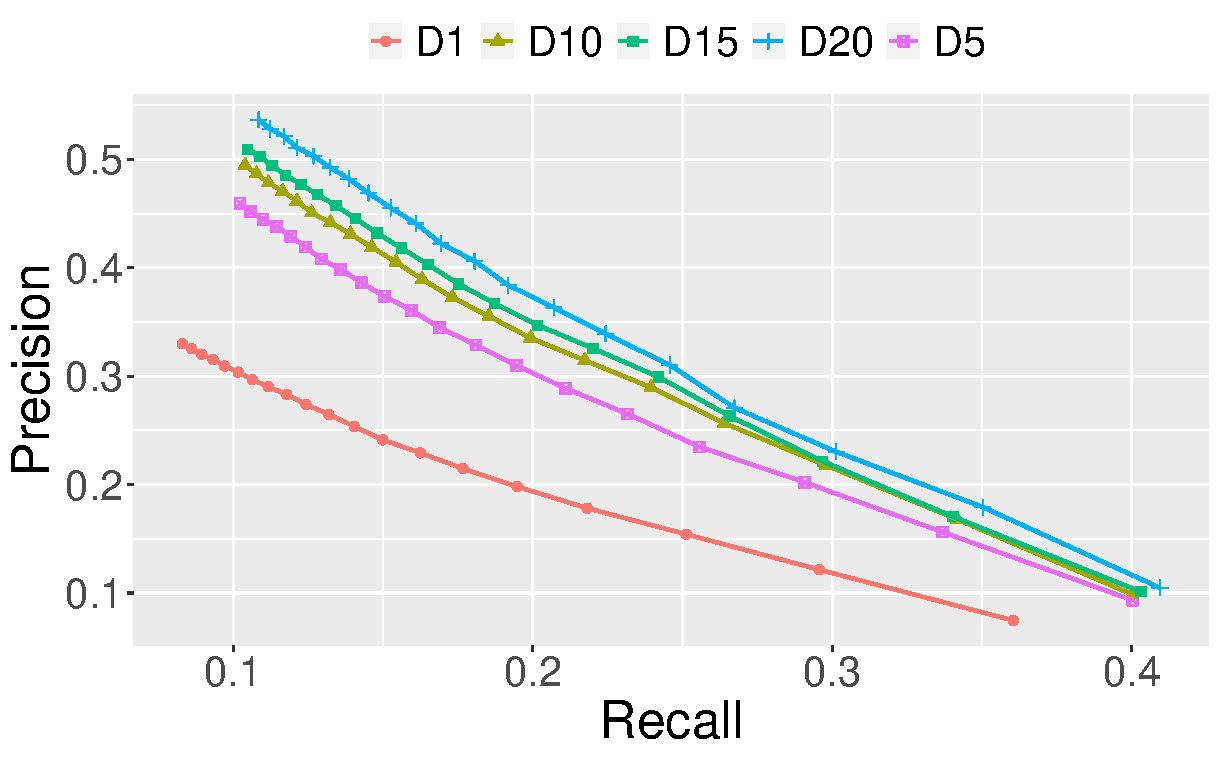
\includegraphics[width=\linewidth]{figs/PrecisionRecallCurve.pdf}
	\caption{Evaluation of the different configuration.}
	\label{fig:configs}
\end{figure}


As we are relying on a collaborative filtering technique, the number of input topics plays an important role in the assessment. Thus, we variate this additional parameter and compute the success rate for 5 and 10 input topics. Figure \ref{fig:success5} and \ref{success10} show the outcome of this comparison.  

\begin{figure}[t!]
	\centering
	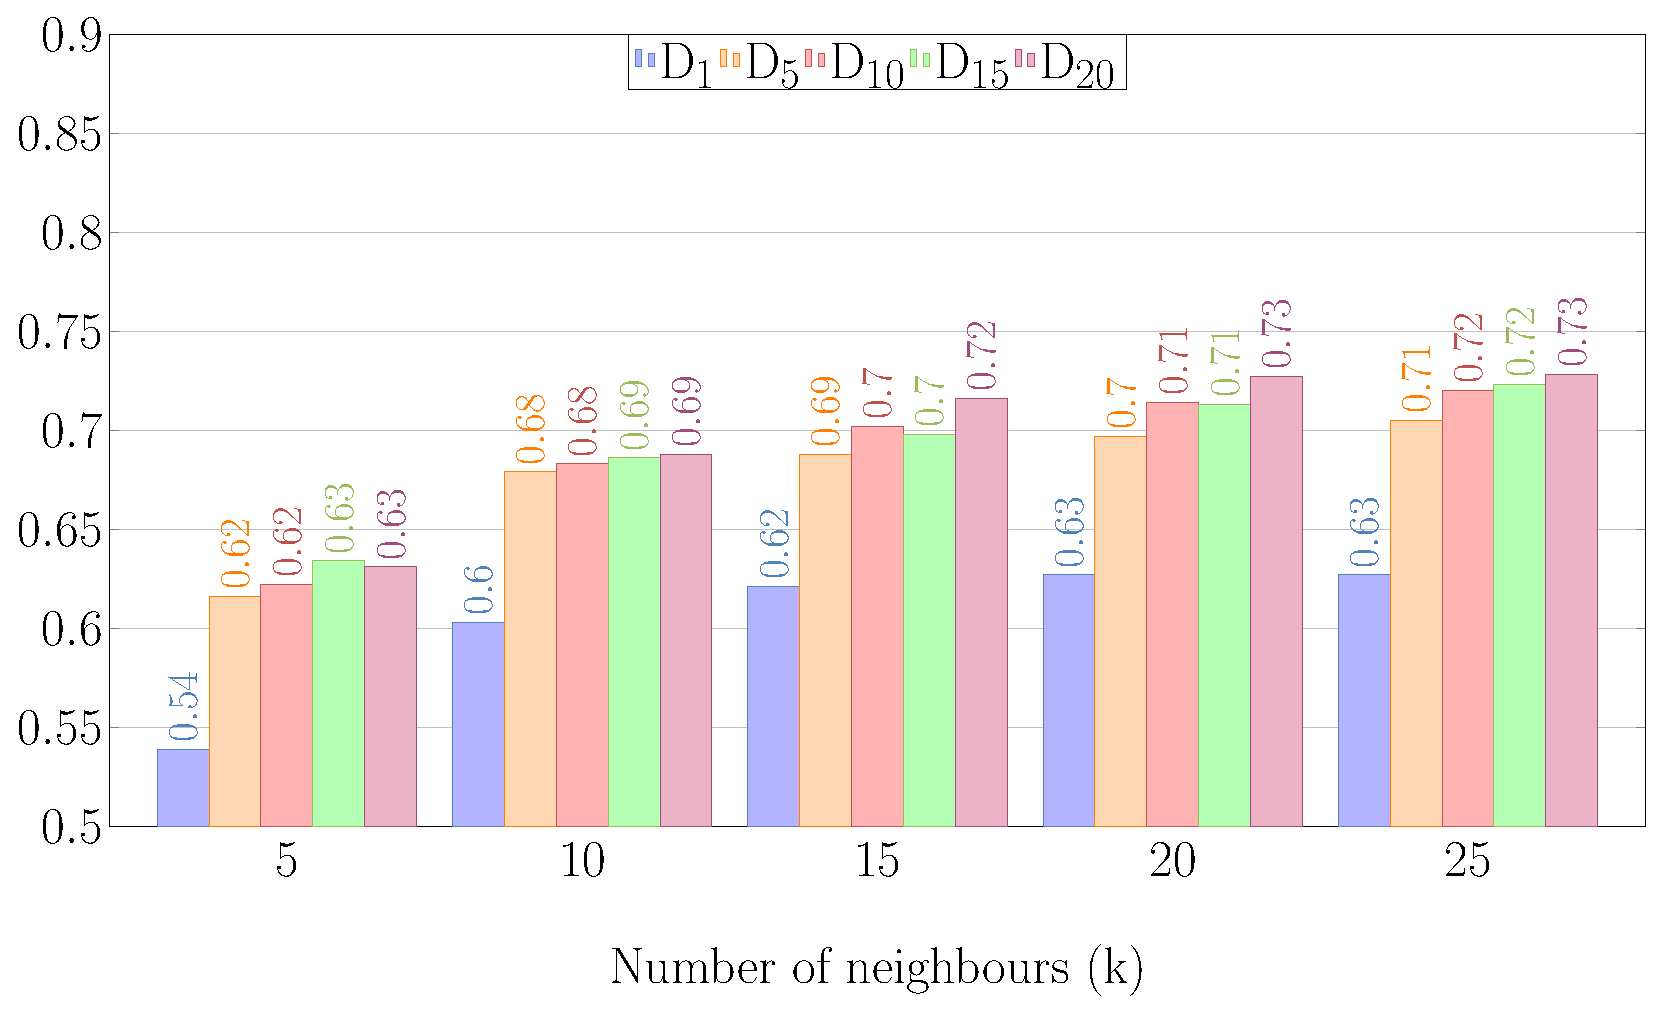
\includegraphics[width=\linewidth]{figs/successRateN@5.pdf}
	\caption{Success rate with 5 input topics.}
	\label{fig:success5}
\end{figure}


\begin{figure}[t!]
	\centering
	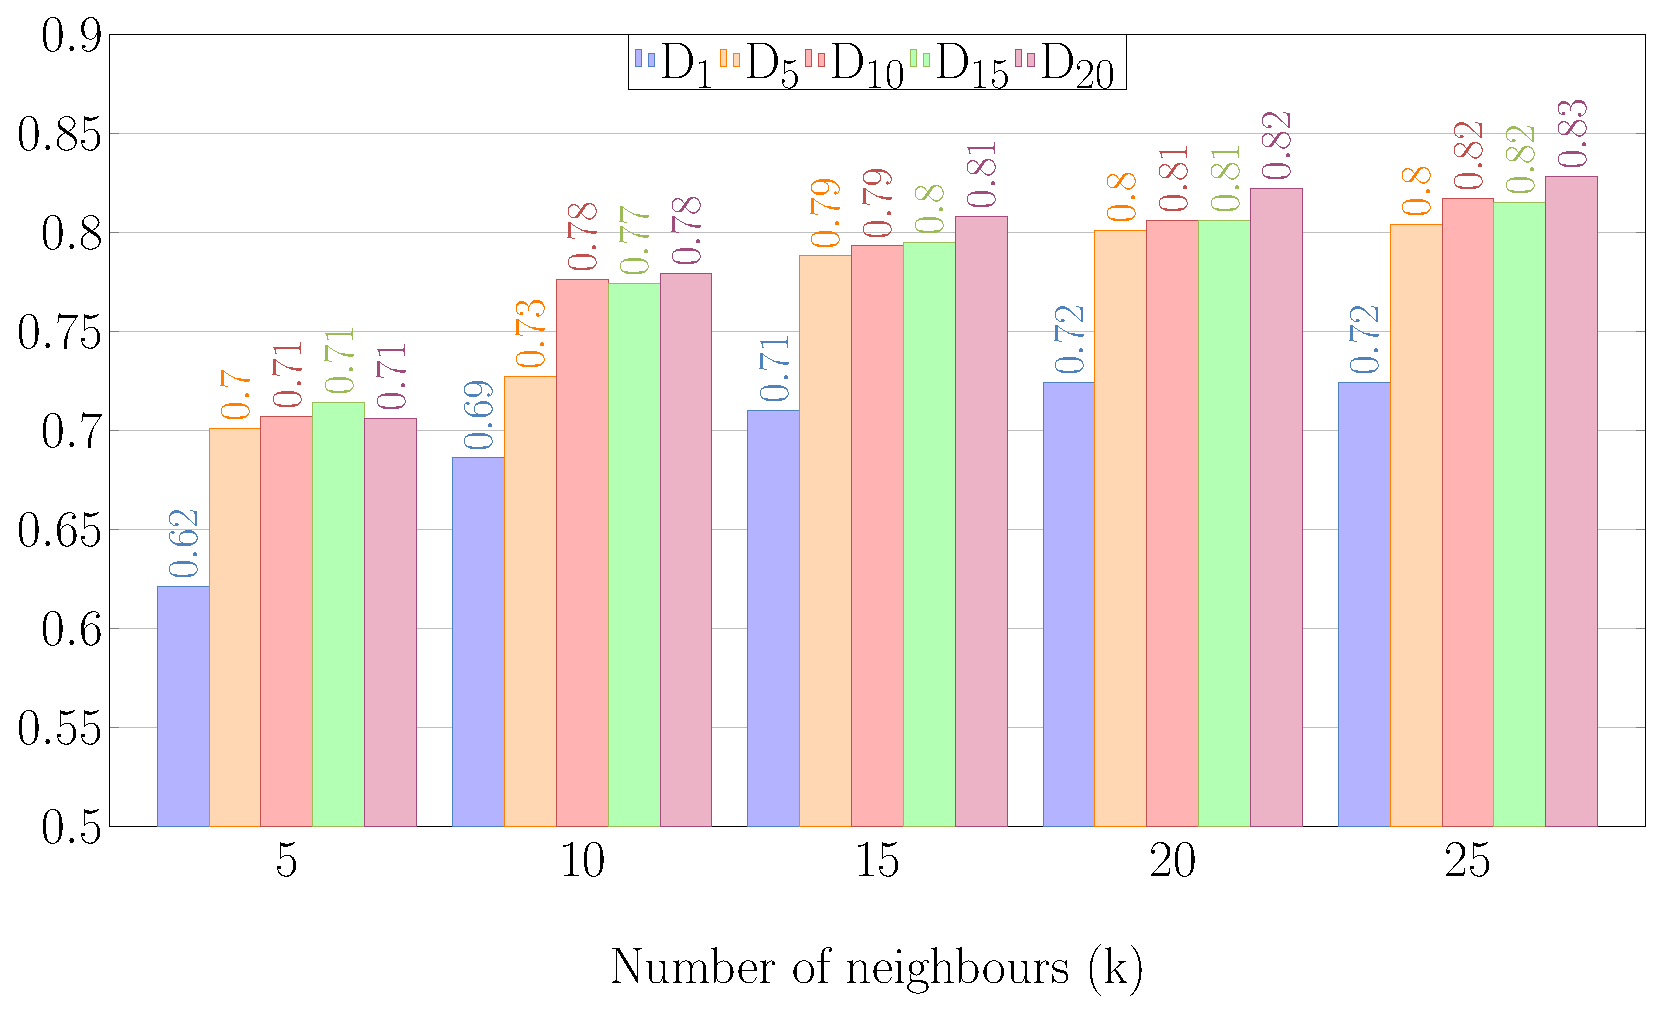
\includegraphics[width=\linewidth]{figs/successRateN@10.pdf}
	\caption{Success rate with 10 input topics.}
	\label{fig:success10}
\end{figure}

As expected, an increasing number of input topics leads to better performance. The success rate assessment exhibits an average improvement of 10\% considering the best number of neighbors \ie k=25. We also demonstrate that the topic filtering preprocessing fosters this enhancement. 



\subsection{\MNB evaluation} \label{sec:EXP2}

\rqsecond

Due to the lack of a baseline, we investigate the prediction performances of the \MNB to compare its outcomes with \CT. Reversely to our previous paper, we extend the \MNB recommendation to not featured topics leaving the underlying structure untouched. This is necessary to undertake a fair comparison with \CT. Table \ref{tab:compareMNB} shows the evaluation results in terms of the already described metrics. 


\begin{table}[h]
\centering


\resizebox{8.5cm}{!} {
\begin{tabular}{|l|l|l|l|l|l|l|}
\hline
  & \multicolumn{3}{c|}{\MNB}          & \multicolumn{3}{c|}{\CT}        \\ \hline
No. of input & Success rate & Precision & Recall & Success rate & Precision & Recall \\ \hline
2  &       0.220       &    0.117       &  0.031       &     0.554         &      0.350     &   0.179      \\ \hline
 4 &     0.392         &    0.119       &     0.063   &       0.682       &       0.267    &   0.271     \\ \hline
6 &    0.538          &      0.122	     &   0.096     &     0.754         &    0.224       &   0.339     \\ \hline
8 &    0.648          &  0.119         &   0.125      &         0.803     &     0.192      &   0.384     \\ \hline
10 &      0.711        &    0.112       &   0.147     &      0.828        &   0.169        &    0.422    \\ \hline
12 &     0.765         &      0.112     &   0.177     &        0.851      &     0.153      &     0.455   \\ \hline
14 &      0.815        &    0.119       &   0.220     &    0.863          &   0.139         &   0.482     \\ \hline
16 &       0.853       &     0.112      &     0.258   &        0.879      &   0.127        &   0.503     \\ \hline
18 &      0.874        &     0.122      &     0.290   &       0.886       &     0.117      &    0.521    \\ \hline
20 &     0.891         &    0.121       &    0.320    &      0.892        &   0.117        &       0.537 \\ \hline
\textbf{Average values} &     0.651        &    0.120       &    0.165   &      0.785        &   0.194        &       0.397  \\ \hline
\end{tabular}
}
\caption{Comparison of the two approaches.}
\label{tab:compareMNB}
\end{table} 


We evaluate both approaches by variating the number of input topics. 
As we can see, \CT outperforms the \MNB considering all the metrics. In particular, the recall values have an improvement of 20\% on average. Considering the \MNB results, the accuracy is very low as we consider in the prediction phase also not featured topics. In the previous paper, we have limited our selves to feature topics due to the model's internal construction. This comparison proves that \CT is more suitable to recommend different topics, even they belong to not featured ones. However, the accuracy is very low compared with the success rate. This could be affected by the similarity function embedded in the recommendation engine. 

\subsection{Entangled evaluation} \label{sec:EXP3}
\rqthird

As a further experiment, we combined the two approaches to investigate potential improvements. We create this \emph{entagle} by feeding \CT with the first top-N results of the \MNB. This simulates the exact use case of the collaborative filtering approach, in which the developer is represented by the \MNB. Table \ref{tab:combined} summarizes the results of this experiment by comparing \CT and the entangled approach. 



\begin{table}[h]
\centering


\resizebox{8.5cm}{!} {
\begin{tabular}{|l|l|l|l|l|l|l|}
\hline
  & \multicolumn{3}{c|}{\CT}          & \multicolumn{3}{c|}{Entangled approach}        \\ \hline
No. of input & Success rate & Precision & Recall & Success rate & Precision & Recall \\ \hline
1  &       0.409       &    0.409       &  0.105       &     0.138         &      0.221     &   0.029      \\ \hline
 2 &     0.554         &    0.350       &     0.179   &       0.220       &       0.198    &   0.053     \\ \hline
3 &    0.632          &      0.301	     &   0.230     &     0.304         &    0.192       &   0.077     \\ \hline
4 &    0.682          &  0.267         &   0.271      &         0.393    &     0.186      &   0.099     \\ \hline
5 &      0.728        &    0.246       &   0.310     &      0.479        &   0.183        &    0.122    \\ \hline
6 &     0.754         &      0.224     &   0.339     &        0.983      &     0.278      &     0.225   \\ \hline
7 &      0.778        &    0.207       &   0.363     &    0.999          &   0.340         &   0.322     \\ \hline
8 &       0.803       &     0.192      &     0.384   &        1      &   0.371        &   0.40     \\ \hline
10 &      0.828        &     0.169      &     0.422   &       1       &     0.382      &    0.511    \\ \hline
15 &     0.872         &    0.132       &    0.493    &      1        &   0.322       &       0.636 \\ \hline
20 &     0.892         &    0.117       &    0.537    &      1        &   0.266        &       0.696 \\ \hline
\textbf{Average values} &     0.785        &    0.194       &    0.397   &      0.826        &   0.296        &       0.433  \\ \hline
\end{tabular}
}
\caption{Results for the entangled approach.}
\label{tab:combined}
\end{table} 














Looking at the results, \CT gains notable improvements. 



%This section reports and discusses the results of our study by addressing the research questions formulated in Section \ref{sec:Evaluation}. \revised{The section is structured into the following subsections.~\Cref{sec:Example} introduces an example of the recommendation results by \LR and \CR.} In~\Cref{sec:ResultAnalysis}, we analyze the obtained results to study the systems' performance. Finally,~\Cref{sec:ThreatsToValidity} discusses the probable threats to validity of our findings. 
%
%
%
%\subsection{Explanatory Example} \label{sec:Example}
%Before addressing our research questions, we illustrate the recommendations of \CR through a running example, \ie the project  \textit{peakgames/libgdx-stagebuilder}  hosted on GitHub.
%As shown in Table \ref{tab:Example}, such a project uses $16$ libraries, which are listed on the left-hand side of the table. Among $16$ included libraries, $8$ items are extracted and used as the ground-truth libraries that are shown in gray. The remaining $8$ items are used as inputs for similarity computation and recommendation, or query. The output obtained by each system is a ranked list in descending order of recommendations with real scores. We took the first $10$ libraries, removed the scores and kept only the order of the list to present the results as in Table~\ref{tab:Example}. The top-$10$ items are then matched against the ground-truth data. 
%%Among $10$ suggested libraries, there are $1$ and $5$ hits by \LR and \CR, respectively, and they are shown in Table~\ref{tab:Example} in bold face. 
%The column \textbf{Freq.} reports the frequency of occurrence of the 
%recommended library, over the set of $1,200$ projects. In this case, \LR 
%only matches \textbf{junit:junit} with the ground-truth (which is obviously used 
%by many projects for testing purposes) but, as we can notice, \CR 
%matches $4$ more projects with the ground-truth. % \MAX{consists or uses?} of
%
%\begin{table}[t!]
	%	\vspace{-.2cm}
	%\caption[Summary]{Recommendation results.}
	%	\vspace{-.4cm}
	%\scriptsize
	\centering	
	\begin{tabular}{|p{0.30cm}|p{6.00cm}|p{0.60cm}|p{4.60cm}|p{0.50cm}|}  \hline		
	a&a&a&a&a
	\end{tabular}	
	\label{tab:Example}
	%\vspace{-.2cm}
\end{table}
%
%Both \LR and \CR obtain a \emph{success rate@10=1.0}. However, \CR has a better \emph{recall@10} compared to \LR as it returns more relevant items (see Eq.~\eqref{eqn:Recall}). Furthermore, among the matches by \CR, $4$ items appear in the top rows of the ranked list, indicating that \CR recommends with a high \emph{precision@N} (see Eq.~\eqref{eqn:Precision}). \LR returns only $1$ relevant item, which means that both \emph{precision@N} and \emph{recall@N} are considerably lower compared to those of \CR. Furthermore, \LR tends to suggest very popular libraries: $6$ out of $10$ items recommended by \LR are used by more than $200$ projects. For instance, besides \textbf{junit:junit}, the second highest frequency item is \textbf{org.slf4j:slf4j-api} ($473/1,200$). By performing an investigation on the outcome of all queries, we realized that \LR usually recommends very popular items. The reasons for such differences are explained in Section~\ref{sec:ResultAnalysis}.
%
%%\PN{This section aims to explain why Novelty is important}
%Four out of five items recommended by \CR have a low frequency of occurrence. For instance, the first item in the 
%ranked list is \textbf{com.badlogicgames.\ gdx:gdx-platform} and this library is included in only $3/1,200$ projects. 
%Referring to Fig.~\ref{fig:NumOfLibsD3}, it is evident that the top $3$ items belong to the long tail, \ie they are 
%extremely unpopular since each is used by only $3$ projects. However, they turn out to be useful as all of them match 
%those stored as ground-truth. In contrast to some existing studies which choose to recommend only popular items to 
%developers \cite{Ponzanelli:2014:MST:2597073.2597077},\cite{Moreno:2015:IUT:2818754.2818860} we see that popularity is not
%a good indicator for selecting a library. This implies that the novelty of a ranked list is important: a system should 
%be able to recommend libraries that are \emph{novel} \cite{Castells_noveltyand}, \ie those that have been rarely seen. 
%In this sense, we expect that \CR can produce good outcomes, not only in terms of success rate and accuracy, but 
%also sales diversity and novelty. 
%
%In summary, for the explanatory example, \CR obtains a comparable success rate, but better accuracy and novelty than \LR. This also confirms that success rate is not sufficient for evaluating the recommendation outcomes. A good recommender system is the one that can maintain a trade-off by improving diversity, novelty but still retaining a good accuracy \cite{Ragone:2017:SLF:3019612.3019837}. Consequently, it is necessary to investigate if this trade-off is guaranteed by \LR and \CR, and this is done in the next sub-sections by considering the whole dataset discussed in the previous section.
%
%
%
%%====================================================================================================================================
%%. In this sense, we see that.  exploit popularity as a means to recommend
%%``long tail''
%%they are far apart from each other in the ranked list, thereby resulting in low precision. %Referring to Table~\ref{tab:FreqDeps}, we see that $7$ out $10$ items recommended by \LR belong to the most popular libraries, whereas the corresponding figure of \CR is $4$. In other words, most of the items recommended by \LR do not fall into the long tail, thus yielding a low novelty for the recommendations.
%
%%According to \emph{Ragone et al.} , 
%%all the testing folds to see
%%\todo[size=\tiny, color=green!40]{Nr. 2: Project without popular 3rd party libs}\footnote{\url{https://github.com/inovait/neatle}}
%%====================================================================================================================================
%%The same set of data is provided as input for \LR and \CR. 
%% (Table \ref{tab:Example})
%%Among other recommended items by \CR which are not a match, \href{https://mvnrepository.com/artifact/commons-collections/commons-collections}{\textbf{commons-collections:commons-collections}} is \emph{"a project to develop and maintain collection classes based on and inspired by the JDK collection framework."} Meanwhile, \href{https://github.com/guoguibing/librec}{\textbf{guoguibing/librec}} is a project that implements various recommendation algorithms. We see that, the library might be useful for the running project.
%%This library we see that
%%and we are going to explain the results in the following sub-sections.  are able to maintain the trade-off
%%Nevertheless, the novelty for this input project is low by both systems. 
%%As already suggested, it is important to maintain a trade-off between. 
%%In a good recommender system there should be a trade-off between accuracy and diversity. diversity should be improved while maintaining adequate accuracy.
%%By manually investigating several queries, we notice that \CR can produce more relevant recommendations in the beginning of the list.
%%Also by comparing with the list of   
%%can recommends the items  %The results are presented in Table \ref{tab:Example}. The asterisk next to the libraries in the third column indicates that it matches against one of the items in the ground-truth libraries. %libraries printed in bold are the matches.
%%\cellcolor{Gray} 
%%====================================================================================================================================
%
%
%
%
%
%
%\subsection{Empirical Study Results} \label{sec:ResultAnalysis}
%
%%\color{blue}
%
%\revised{In this section, we report the results by addressing the research questions \textbf{RQ$_1$}, \textbf{RQ$_2$}, \textbf{RQ$_3$}, \textbf{RQ$_4$}, and \textbf{RQ$_5$}.}
%
%%discrepancies.
%
%\vspace{.1cm}
%%\noindent\textbf{RQ$_1$:} \emph{Does \CR obtain a better success rate compared to \LR?}
%\noindent \revised{\rqfirst}
%\vspace{-.05cm}
%
%%The original dataset consists of. 
%%, (\eg)
%
%
%
%\noindent%N (the cut-off value for the list of items to be recommended) 
%%\emph{Success rate:}  %We are interested in understanding the. We concentrate on comparing \CR with \LR. In the following section.
%%\paragraph{\textbf{Success rate}} 
%% answer this question
%%To compare \CR with \LR, 
%
%
%\paragraph{\textbf{Comparison between \LR and \CR}} We performed a series of experiments on \code{D1} using different combinations of number of recommended libraries (\ie $N$), and number of neighbor projects exploited in the recommendation phase (\ie $k$). Varying $N$ means changing the length of the recommendation list, whereas increasing $k$ means considering more neighbor projects for recommendation.
%
%
%\begin{figure*}[h!]
%	\centering
%	
%	\begin{tabular}{c c}	
%		\centering    
%		\subfigure[Success rate@5, 
%		k=\{5,10,15,20,25\}]{\label{fig:RecallRate5}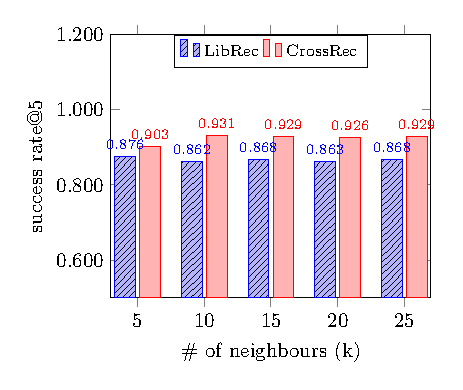
\includegraphics[width=0.48\textwidth]{figs/RecallRate@5.pdf}}		& 	
%		\subfigure[Success rate@10, k=\{5,10,15,20,25\}]{\label{fig:RecallRate10}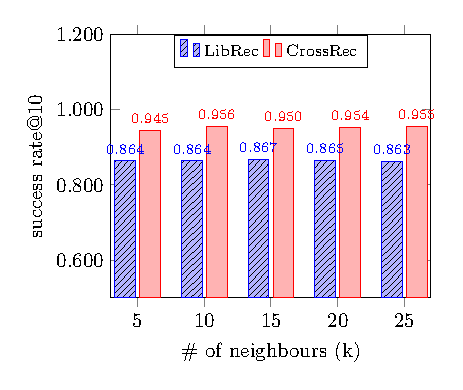
\includegraphics[width=0.48\textwidth]{figs/RecallRate@10.pdf}}\\
%		\subfigure[Success rate@\{1,3,5,7,10\}, k=10]{\label{fig:RecallRateNk10}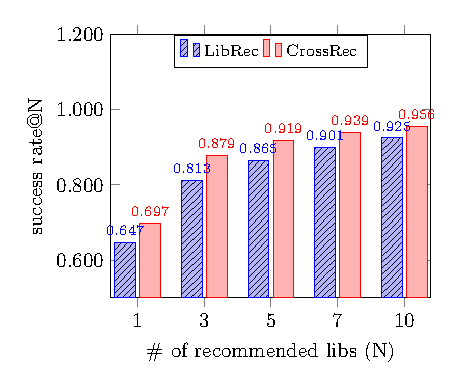
\includegraphics[width=0.48\textwidth]{figs/RecallRate@N_k10.pdf}}	& 	
%		\subfigure[Success rate@\{1,3,5,7,10\}, k=20]{\label{fig:RecallRateNk20}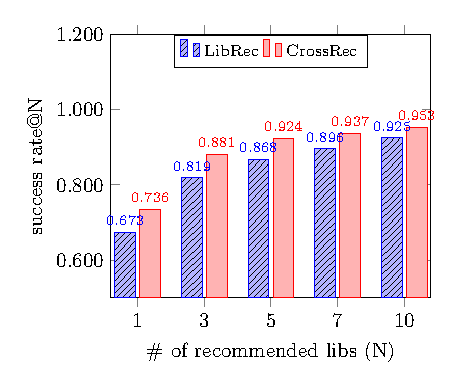
\includegraphics[width=0.48\textwidth]{figs/RecallRate@N_k20.pdf}}\\
%	\end{tabular}
%	\label{fig:RecallRate}
%	\caption{Success rate of \CR and \LR on \code{D1}.}
%\end{figure*}
%
%
%Fig.~\ref{fig:RecallRate5} shows the \emph{success rate@5} for k=\{5, 10, 15, 20, 25\}. As it can be seen there, the success rate values obtained by \CR are always superior to those of \LR. The maximum \emph{success rate@5} of \LR is $0.876$, whereas \CR obtains success rates being greater than $0.903$ for all configurations, with $0.931$ being the maximum value. Fig.~\ref{fig:RecallRate10} shows the \emph{success rate@10}, for this setting, \LR gains a comparable performance for $N=5$. Meanwhile, \CR achieves a slight improvement in its performance compared to the case with $N=5$. It is evident that \CR outperforms \LR in all test configurations. Fig.~\ref{fig:RecallRate5} and Fig.~\ref{fig:RecallRate10} imply that changing the number of neighbor projects $k$ does not make a substantial difference in their match rate, as \emph{success rate@N} is stable towards $k$ for both systems.
%
%Next, we investigate the success rate with regards to $N$. We consider a small number of recommended items, \ie $N=\{1,3,5,7,10\}$. In practice, this means that the developer wants to see a short list of recommended libraries. In the first experiment, $k$ is fixed to $10$ and the outcomes are depicted in Fig. \ref{fig:RecallRateNk10}. For $N=1$, \LR achieves a success rate of $0.647$ which is lower than the corresponding value $0.697$ produced by \CR. A success rate of $0.697$ implies that \CR can supply relevant recommendations to the developer at an encouraging match rate, even when she expects only an extremely brief list. Once $k$ is changed from $10$ to $20$, both systems have a slight increase in \emph{success rate@1} as depicted in Fig. \ref{fig:RecallRateNk20}. However, for other values of $N$, there are almost no changes in success rate. To further observe this behavior, we conducted more experiments with an increasing $k$, \eg $k=\{50,60,100\}$. As far as we can see, there are no subtle differences between the conclusions obtained from the new experiments with those previously presented in the paper. Thus, for the sake of clarity, the outcomes of these experiments are omitted from the paper.
%
%%Nevertheless, the outcomes of these experiments are omitted from the paper due to space limitation. We noticed that considering more similar projects for recommendation does not improve success rate. %When we consider a bigger value of $N$, starting from $N=5$, \CR gains a quick increase in its performance as the success rates are always greater than $0.924$. 
%
%%Last but not least, t
%
%
%%The second column of Table \ref{tab:Wilcoxon} and of Table \ref{tab:Cliff} 
%
%%To see if the improvement of the proposed approach is statistically significant and substantial, we perform a Wilcoxon rank sum test \cite{Wilcoxon1992} on all the quality scores for both systems, using $k=10$ and $N=\{3,5,10,15\}$. The $p$-values for all quality metrics are shown in Table~\ref{tab:Wilcoxon}. The null hypothesis is that there are no differences between the performance of \CR and that of \LR. Using $5\%$ as the confidence level, we see that by all quality indicators the \emph{p-values} are always lower than $5 \times e^{-2}$. Cliff's $d$ values are reported in Table \ref{tab:Cliff}. As the table shows, the observed differences are always in favor of \CR (\ie effect sizes are always positive). Magnitude of the computed Cliff's $d$ is small for precision and recall, while it is large for all other indicators, including Success Rate.
%%
%%\begin{tcolorbox}
%%In this sense, we reject the null hypothesis and conclude that the performance improvement obtained by \CR is statistically significant. %or \emph{p-value} $< 5 \times e^{-2}$ . in terms of all quality metrics. 
%%\end{tcolorbox}
%
%
%\begin{table*}[ht]
%	\footnotesize	
%	\color{blue}
%	\caption{Wilcoxon rank sum test adjusted $p$-values and Cliff's $d$ results for N=\{3,5,10,15\}, k=10.}
%	\centering
%	\begin{tabular}{|p{4.3cm}|p{1.0cm}|p{1.0cm}|p{1.0cm}|p{1.0cm}|}\hline
%	%	\rowcolor{verylightgray}
%		& \multicolumn{4}{c|}{\textbf{Cut-off value (N)}}         \\ \hline
%		\textbf{Test} & 3	 & 5   & 7     & 10    \\ \hline
%		Wilcoxon r.s.t. adjusted $p$-values  & 0.02 & 0.02 & 0.17 & 0.002  \\ \hline
%		Cliff's $d$ results   &  0.70 (l) & 0.74 (l) & 0.93 (l) & 0.58 (l) \\ \hline
%	\end{tabular}
%	\label{tab:WilcoxonCliffLibRecCrossRec}
%	\color{black}
%\end{table*}
%
%\revised{Table \ref{tab:WilcoxonCliffLibRecCrossRec} reports Wilcoxon rank sum test adjusted $p$-values and Cliff's $d$, respectively for the comparison of \LR and \CR in terms of {\em success rate}, using $k=10$ and $N=\{3,5,10,15\}$; the labels in parentheses indicate the magnitude (n:negligible, s:small, l:large). As the table shows, the differences are always statistically significant and in favor of \CR (effect size is positive), with a large effect size.}
%
%
%\begin{tcolorbox}[boxrule=0.86pt,left=0.3em, right=0.3em,top=0.1em, bottom=0.05em]
%	%	\color{blue}
%	%	\revised{
%	\small{In summary,  \CR significantly outperforms \LR in all considered test configurations concerning \emph{success rate}, with a large effect size. The recommendation time for a fold (120 projects) is relatively faster for \CR (3s) than for \LR (20s).}%}%  \CR can reach a high performance when.
%\end{tcolorbox}
%
%
%
%%We also measured the average time needed to generate, 
%%We analyzed the dataset\footnote{\url{http://sel.ist.osaka-u.ac.jp/people/ali/libRecommendation/}} exploited to evaluate \LF~\cite{Ouni:2017:SSL:3032135.3032325}. 
%%We varied the number
%%on-the-fly’ recommendations in such a way that the developer will be automatically notified by relevant libraries while he is writing his code
%%|p{0.8cm}|
%%\LF was evaluated using different metrics, however in our work we are interested in comparing. 
%
%%We performed experiments on \code{D2} to. 
%% when N increases
%%a high performance is favored and helps developers approach relevant libraries
%
%\paragraph{\textbf{\revised{Comparison between \LF and \CR}}} \revised{Even though \LF is a bit different from \CR as it aims at providing \emph{on-the-fly} recommendations while the developer is coding by exploiting the existing semantic, we attempted to compare \CR with \LF by applying the same experimental settings. A comparison between \LF and \CR is depicted in Table~\ref{tab:SuccessRateLibFinderCrossRec}.\footnote{\revised{The success rates of \LF were extracted directly from the paper~\cite{Ouni:2017:SSL:3032135.3032325}}.} For small cut-off values, \ie $N=\{1,2,4\}$, \CR obtains a better success rate than \LF does. However, by the higher values $N=\{6,8,10\}$, \LF gains an improvement in its performance. This suggests that \LF tends to provide matches quite late in the ranked list. On one hand, a system with such a recommendation list helps developers approach relevant libraries. On the other hand, this is not useful for those who prefer to get only a short list of recommendations.}
%
%
%%\revised{
%\begin{table*}[ht]
%	\footnotesize	
%	\color{blue}
%	\caption{Success rate of \LF and \CR on \code{D2}.}
%	\centering
%	\begin{tabular}{|p{1.5cm}|p{1.0cm}|p{1.0cm}|p{1.0cm}|p{1.0cm}|p{1.0cm}|p{1.0cm}|}\hline
%		%\rowcolor{grey}
%		& \multicolumn{6}{c|}{\textbf{Cut-off value (N)}}         \\ \hline
%		\textbf{System} & 1	 & 2   & 4      & 6   & 8    &  10          \\ \hline
%		\LF  & 0.633 & 0.698 & 0.813 & \textbf{0.876} & \textbf{0.904} & \textbf{0.918}  \\ \hline
%		\CR  & \textbf{0.771} & \textbf{0.816} & \textbf{0.851} & 0.860 & 0.863 & 0.864  \\ \hline
%	\end{tabular}
%	\label{tab:SuccessRateLibFinderCrossRec}
%	\color{black}
%\end{table*}
%%}
%
%% with a certain level of maturity
%% which cannot be used as input for the splitting
%% with different levels of maturity
%
%\revised{By carefully examining the \code{D2} dataset, we realized that there are several projects containing a small number of dependencies, \eg 1 or 2 third-party libraries. Such projects are not beneficial to the training of \CR since the corresponding metadata is not sufficient to compute similarity and, consequently, to provide a recommendation (see Eq.~\eqref{eqn:TFIDF} and Eq.~\eqref{eqn:VsmSim}). Thus, to further investigate the performance of \CR on~\code{D2}, we performed a filtering step as follows. Starting from the dataset, we selected projects containing a certain number of libraries, and such a number is called as $L$. The number was then varied to create different configurations. In practice, this means that we consider only mature projects, \ie those that include a decent number of libraries for training. Table~\ref{tab:SuccessRateCrossRecD1} shows the success rate obtained by varying $L$. As it can be seen, CrossRec's performance is proportional to $L$: the more dense (with respect to dependencies) the projects are, the better performance \CR achieves. For instance, when we consider only projects with at least $4$ libraries, \ie $L=4$ the success rate obtained for $N=10$ is $0.914$. However, if $L$ is increased to $10$, the corresponding success rate improves to reach $0.987$. The same trend can be witnessed by other combinations of $L$ and $N$.} %Thus, the first conclusion to be drawn is that \CR is able to work on a large datasets and provide accurate recommendations.} % achieves much better performance when.
%
%%\revised{
%\begin{table*}[ht]
%	\footnotesize
%	\color{blue}
%	\caption{Success rate of \CR on \code{D2} with different number of libraries ($L$).}
%	\centering
%	%	\begin{tabular}{|r|r|r|r|r|r|r|}\hline
%	\begin{tabular}{|p{0.75cm}|p{0.75cm}|p{1.0cm}|p{1.0cm}|p{1.0cm}|p{1.0cm}|p{1.0cm}|p{1.0cm}|}\hline
%		%\rowcolor{verylightgray}
%		\multicolumn{2}{|c|}{} & \multicolumn{6}{c|}{\textbf{Cut-off value (N)}}         \\ \hline%\cline{3-8}
%		%		\rowcolor{verylightgray}
%		\multicolumn{2}{|c|}{\textbf{\# of libraries}} & 1	 & 2   & 4    & 6   & 8    &  10          \\ \hline
%		{\multirow{4}{*}{$L$}} & 4          & 0.811 & 0.853 & 0.894 & 0.906 & 0.911 & 0.914  \\ \cline{2-8}
%		& 6          & 0.890 & 0.926 & 0.948 & 0.958 & 0.961 & 0.964  \\ \cline{2-8}
%		& 8          & 0.930 & 0.958 & 0.972 & 0.977 & 0.982 & 0.986  \\ \cline{2-8}
%		& 10         & 0.938 & 0.964 & 0.976 & 0.981 & 0.984 & 0.987  \\ \hline
%	\end{tabular}
%	\label{tab:SuccessRateCrossRecD1}
%	%\vspace{-.1cm}
%	\color{black}
%\end{table*}
%%}
%
%
%%=====================================================================================
%% has been neglected by LibFinder
%%Finally, we also incorporate libraries' version. 
%% is not used in the evaluation
%%which is a limitation of LibFinder. 
%%neglects 
%%The final dataset consists of 5,102 projects and. 
%%Furthermore, \CR is able to recommend library version, 
%%as stated in the original paper~\cite{Ouni:2017:SSL:3032135.3032325}
%%\CR transcends the limitation of \LF since it is capable of recommending libraries with versions. Moreover, \CR obtains a better performance when the input data is dense, \ie more libraries are available for training.
%%We come to the conclusion that o
%%in Table~\ref{tab:SuccessRateCrossRecD2Version}
%%=====================================================================================
%
%
%\revised{While the \code{D2} dataset also specifies library versions,
%	\LF is unable to deal with this information, resulting in a limitation, as already stated by the authors~\cite{Ouni:2017:SSL:3032135.3032325}. In practice, it is crucial to provide developers with not only a suitable library, but also a specific version of that library, otherwise there might be some issues related to version compatibility~\cite{Mileva:2009:MTL:1595808.1595821} or, in general, recommending obsolete libraries. Thus, we injected also library version into the training and testing data and fed it to \CR. The final results for different configurations are reported in Table~\ref{tab:SuccessRateCrossRecD2Version}.} \revised{As it can be seen in the table, given that decent training data is available, \CR also recommends libraries with version, achieving a high success rate. For instance, even when projects containing at least 2 libraries are considered, or $L=2$, \CR obtains a success rate of $0.620$ for $N=1$. This quality metric improves linearly alongside $L$ and $N$. As an example, when $L=10$ and $N=10$, the corresponding success rate is $0.955$.}
%
%
%
%	\begin{table*}[ht]
%		\footnotesize
%		\color{blue}
%		\caption{Success rate of \CR on \code{D2} when library version is considered.}
%		\centering
%		%	\begin{tabular}{|r|r|r|r|r|r|r|}\hline
%		\begin{tabular}{|p{0.75cm}|p{0.75cm}|p{1.0cm}|p{1.0cm}|p{1.0cm}|p{1.0cm}|p{1.0cm}|p{1.0cm}|}\hline
%%			\rowcolor{gray}
%			\multicolumn{2}{|c|}{} & \multicolumn{6}{c|}{\textbf{Cut-off value (N)}}         \\ \hline%\cline{3-8}
%			%		\rowcolor{verylightgray}
%			\multicolumn{2}{|c|}{\textbf{\# of libraries}} & 1	 & 2   & 4    & 6   & 8    &  10          \\ \hline
%			{\multirow{4}{*}{$L$}} & 2 	& 0.620 & 0.676 & 0.715 & 0.729 & 0.735 & 0.738  \\ \cline{2-8}
%			& 4                    		& 0.785  & 0.834 & 0.872 & 0.893 & 0.903 & 0.907  \\ \cline{2-8}
%			& 6                    		& 0.848 & 0.885  & 0.907 & 0.921 & 0.931 & 0.936  \\ \cline{2-8}
%			& 8                    		& 0.888 & 0.919 & 0.931 & 0.937 & 0.945 & 0.950  \\ \cline{2-8}
%			& 10                   		& 0.906 & 0.930 & 0.944 & 0.948 & 0.951 & 0.955  \\ \hline
%		\end{tabular}
%		\label{tab:SuccessRateCrossRecD2Version}
%		\color{black}
%		%\vspace{-.1cm}
%	\end{table*}
%
%
%\begin{tcolorbox}[boxrule=0.86pt,left=0.3em, right=0.3em,top=0.1em, bottom=0.05em]
%	%	\color{blue}
%	\revised{
%		\small{On the \code{D2} dataset, \CR obtains a comparable performance compared to that of \LF. When it comes to a dataset containing projects with more libraries, \CR is able to give more precise recommendations. Differently from \LF, \CR is capable recommending also a specific version of a library.}}
%\end{tcolorbox}
%
%
%
%
%
%
%\paragraph{\textbf{\revised{Comparison between \LC and \CR}}} \revised{For this 
%	evaluation, we used the same experimental settings utilized to evaluate \LF. In 
%	particular, the following cut-off values have been considered: 
%	$N=\{1,3,5,7,10\}$. According to Table~\ref{tab:SuccessRateD2}, the performance 
%	obtained by \CR is always better than that of \LC.\footnote{\revised{The 
%			success rate values for \LC were extracted from the 
%			paper~\cite{SAIED2018164}}.} For example, when the cut-off value $N=1$, \LC 
%	gets $0.12$ as success rate while the corresponding value by \CR is $0.21$. 
%	Similarly, for other values of $N$, our proposed tool gains a superior 
%	performance compared to that of \LC, in particular when $N=10$, \CR achieves a 
%	success rate which is nearly twice what \LC achieves, \ie $0.42$ compared to 
%	$0.22$.}% \MAX{this is the only case where success rate has 2 digits instead of 
%%3. Maybe because of the data in the original paper?}} \PN{Yes, you are right. 
%%In the original paper, we can find only scores with two digits.}
%
%
%\begin{table*}[ht]
%	\footnotesize
%	\color{blue}
%	\caption{Success rate of \LC and \CR on \code{D3}.}
%	\centering
%	\begin{tabular}{|p{1.5cm}|p{1.0cm}|p{1.0cm}|p{1.0cm}|p{1.0cm}|p{1.0cm}|}\hline
%%		\rowcolor{verylightgray}
%		& \multicolumn{5}{c|}{\textbf{Cut-off value (N)}}         \\ \hline
%		\textbf{System} & 1	 & 3   & 5      & 7   & 10          \\ \hline
%		\LC  & 0.12 & 0.14 & 0.15 & 0.17 & 0.22   \\ \hline
%		\CR  & \textbf{0.21} & \textbf{0.31} & \textbf{0.36} & \textbf{0.39} & \textbf{0.42}   \\ \hline
%	\end{tabular}
%	\label{tab:SuccessRateD2}
%\end{table*}
%
%
%\revised{Similarly to \code{D2}, \code{D3}  also features library versions, however \LC cannot provide version-specific recommendations. For each library in the dataset, we integrated its version and fed as input for \CR. For this experiment, we selected only projects with a considerably high number of third-party libraries, \ie $L=\{7,8,9,10\}$ and the final results are shown in Table~\ref{tab:SuccessRateCrossRecD3Version}.}
%
%
%%\revised{To conform with. For this evaluation, we also. The following cut-off values have been considered: $N=\{1,3,5,7,10\}$. According to Table~\ref{tab:SuccessRateD2}, the performance obtained by \CR is always better than that of \LC. For example, when the cut-off value $N=1$, \LC gets $0.12$ as success rate while the corresponding value by \CR is $0.21$. Similarly, for other values of $N$, \CR gains a superior performance compared to \LC, for example when $N=10$.}
%
%
%	\begin{table*}[ht]
%		\footnotesize
%		\color{blue}
%		\caption{Success rate of \CR on \code{D3} when library version is incorporated.}
%		\centering
%		\begin{tabular}{|p{0.75cm}|p{0.75cm}|p{1.0cm}|p{1.0cm}|p{1.0cm}|p{1.0cm}|p{1.0cm}|}\hline
%%			\rowcolor{verylightgray}
%			\multicolumn{2}{|c|}{} & \multicolumn{5}{c|}{\textbf{Cut-off value (N)}}         \\ \hline%\cline{3-8}
%			\multicolumn{2}{|c|}{\textbf{\# of libraries}} & 1	 & 3   & 5    & 7   & 10          \\ \hline
%			{\multirow{4}{*}{$L$}} & 7 	& 0.215 & 0.313 & 0.361 & 0.392 &  0.423  \\ \cline{2-7}
%			& 8                    		& 0.219 & 0.315 & 0.362 & 0.392 & 0.423   \\ \cline{2-7}
%			& 9                    		& 0.214 & 0.311 & 0.355 & 0.383 &  0.415  \\ \cline{2-7}
%			& 10                        & 0.255 & 0.368 & 0.422 & 0.456 &  0.494  \\ \hline
%		\end{tabular}
%		\label{tab:SuccessRateCrossRecD3Version}
%		\color{black}
%	\end{table*}
%
%%As it can be seen in Table~\ref{tab:SuccessRateCrossRecD3Version}, 
%%the same trend can be witnessed: 
%%Given that decent training data is available, 
%%According to 
%% For instance, even when projects containing at least 2 libraries are considered, or $L=2$, \CR obtains a success rate of $0.620$ for $N=1$.
%% the success rates are.
%% is very small
%
%\revised{Table~\ref{tab:SuccessRateCrossRecD3Version} shows that \CR also recommends specific versions of libraries. Among the configurations, the maximum success rate is $0.494$, and it is reached when $L=10$ and $N=10$. However, in comparison to the outcome by \code{D2}, \CR achieves a considerably lower success rate. Moreover, there is a marginal difference in performance between different values of $L$. Especially, the system's performance suffers a setback when $L=9$ in comparison to $L=8$. By carefully investigating the dataset, we found out that the projects of \code{D2} are very diverse, and they contain a large number of libraries. Moreover, the similarity among the projects is considerably low. This means that the dataset exhibits a high level of heterogeneity and therefore, given a project, generally we cannot find a good set of similar projects. Under the circumstances, it is more difficult to recommend highly relevant libraries, resulting in a low success rate.}
%
%
%%A possible explanation for this is that 
%
%%\begin{tcolorbox}[boxrule=0.86pt,left=0.3em, right=0.3em,top=0.1em, bottom=0.05em]
%%%	\color{blue}
%%	\revised{\small{On the \code{D2} dataset, \CR clearly outperforms \LC. \CR can reach a better performance when.}}
%%\end{tcolorbox}
%
%
%\begin{tcolorbox}[boxrule=0.86pt,left=0.3em, right=0.3em,top=0.1em, bottom=0.05em]
%	\revised{\small{On the \code{D3} dataset, \CR clearly outperforms \LC with respect to various configurations. Furthermore, \CR can recommend also libraries with a specific version, which \LC cannot.}}
%\end{tcolorbox}
%
%
%%====================================================================================================================================
%%filter out the data and retain those projects that.
%
%%\begin{table*}[t]
%%	\footnotesize
%%	\caption{Wilcoxon rank sum test p-values for N=\{3,5,10,15\}, k=10}
%%	\vspace{-.3cm}
%%	\centering
%%	\begin{tabular}{|p{0.5cm}||p{1.60cm}|p{1.80cm}|p{1.50cm}|p{1.50cm}|p{1.50cm}|p{1.50cm}|}
%%		\hline
%%		& \textbf{Success Rate} &     \multicolumn{2}{c|}{\textbf{Accuracy}}      &   \multicolumn{2}{c|}{\textbf{Sales Diversity}}   & \textbf{Novelty}      \\ \hline
%%		\textbf{N} & Success Rate          & Precision               & Recall                & Coverage                  & Entropy               & EPC                   \\ \hline
%%		3          & $8.87 \times e^{-3}$  & $< 2.20 \times e^{-16}$ & $ 5.40 \times e^{-8}$ & $ 1.29 
%%		\times e^{-4}$  & $ 4.33 \times e^{-5}$ & $ 1.08 \times e^{-5}$ \\ \hline
%%		5          & $6.32 \times e^{-3}$  & $< 2.20 \times e^{-16}$ & $3.03 \times e^{-12}$ & $ 4.87 
%%		\times e^{-4}$  & $ 2.16 \times e^{-5}$ & $ 1.08 \times e^{-5}$ \\ \hline
%%		%7         & $4.34 \times e^{-2}$  & $< 2.20 \times e^{-16}$ & $1.58 \times e^{-10}$ & $ 2.08 
%%		%\times e^{-3}$ & $ 2.16 \times e^{-5}$ & $ 7.57 \times e^{-5}$ \\ \hline
%%		10         & $3.69 \times e^{-2}$  & $< 2.20 \times e^{-16}$ & $4.53 \times e^{-12}$ & $ 1.50 
%%		\times e^{-3}$  & $ 1.08 \times e^{-5}$ & $ 7.57 \times e^{-5}$ \\ \hline
%%		15         & $2.87 \times e^{-2}$  & $ 1.10 \times e^{-14}$  & $5.20 \times e^{-10}$ & $ 1.50 
%%		\times e^{-3}$  & $ 2.16 \times e^{-5}$ & $ 2.05 \times e^{-4}$ \\ \hline
%%	\end{tabular}
%%	\vspace{-.2cm}
%%	\label{tab:Wilcoxon}
%%	\vspace{-.2cm}
%%\end{table*}
%%====================================================================================================================================
%
%
%
%
%
%%====================================================================================================================================
%%phenomenon
%%Also in this experiment setting, \CR overtakes \LR concerning recall rate.% as its recall rates. Once we consider Fig. \ref{fig:RecallRateNk10} and Fig. \ref{fig:RecallRateNk20} together,    
%
%%The results obtained from the experiments  are shown in Fig. \ref{fig:RecallRate}. Specifically, Fig. \ref{fig:RecallRate5} and Fig. \ref{fig:RecallRate10} show the \emph{recall rate@5} and \emph{recall rate@10} for $k=\{5,10,15,20,25\}$.  Fig. \ref{fig:RecallRateNk10}, and Fig. \ref{fig:RecallRateNk20}.
%%The value $N=1$ means the developer needs a single library from the recommendation.
%% starting from $N=5$, the recall rates by \CR are always greater than $0.90$.
%%Table \ref{tab:Tenfold_Neighbours} and \ref{tab:Tenfold_Libraries}. Table \ref{tab:Tenfold_Neighbours} lists the average \emph{recall rate@N} for \emph{N=5} and \emph{N=10} with the number of neighbour projects used for recommendation being varied according to \LR, \ie $k=\{5,10,15,20,25\}$. As can be seen, for all combinations of \emph{k} and \emph{N} using either user-based or item-based collaborative filtering, \CR always earns recall rates that are superior to those of \LR. Specifically, for \emph{N=5}, the recall rates range from $0.88$ to $0.92$ by user-based collaborative filtering and from $0.86$ to $0.91$ by item-based collaborative filtering. Referring back to \cite{6671293}, the maximum \emph{recall rate@10} obtained by \LR with the same test configuration is $0.852$ which is inferior to those obtained by \CR. Similarly, for \emph{k=10}, \CR also outperforms \LR as the maximum \emph{recall rate@10} of VsmSim is $0.94$ whereas the corresponding value by \LR is $0.894$.
%%Even when only $5$ neighbour projects are used as input for recommendation, meaning that the \textbf{Recommendation Engine} has very little clue about the test project, \CR still gives a recall rate of $0.88$. This is the minimum value obtained from this test configuration, however it is still better than the best outcome of \LR which is $0.852$.
%%====================================================================================================================================
%% and. %, which is indeed a high score.
%%\begin{table}[h!]w
%%		n		& k=5       & k=10 		\\ \hline	
%%		10      & 0.92      & 0.94      \\ \hline
%%		20      & 0.91      & 0.94      \\ \hline
%%		50      & 0.91      & 0.94      \\ \hline
%%		60      & 0.91      & 0.95      \\ \hline
%%		100     & 0.90      & 0.93      \\ \hline
%%	\end{tabular}
%%	\caption{Average Recall Rate@k for ten-fold cross validatione
%%	\label{tab:Tenfold}
%%\end{table}
%%====================================================================================================================================
%%Next, we consider different number of neighbours, for $k=5$ and $k=10$, the same number of neighbours as in \LR.  different values of $k$ 
%%In conformance with the evaluation performed in \cite{6671293}, we investigate the performance of the system with regards to the number of recommended libraries, \ie $k=\{1,3,5,7,10\}$ and the results are shown in Table \ref{tab:Tenfold_Libraries}. Also in this experiment \CR obtains better recall rates compared to those of \LR. For the case when $N=1$, meaning that the developer wants to see only one library in the recommendation list, \CR still gets a $recall$ $rate@1=0.69$ by user-based collaborative filtering and $0.68$ by item-based collaborative filtering, respectively. These values are higher compared to $0.616$ by \LR. For $N=3$, \CR has a recall rate of $0.89$ which is higher than $0.804$, the corresponding value in \LR. 
%%Taking the best outcomes obtained by \CR, we depict in Fig. \ref{fig:RecallRateK} and Fig. \ref{fig:RecallRateN} together with the results by \LR. The scores for \LR are extracted from the original \LR paper \cite{6671293}.
%%====================================================================================================================================
%%\begin{figure}[h!]
%%	\centering
%%	\includegraphics[width=0.35\textwidth]{figs/RecallRate.pdf}
%%	\caption{Comparison of recall rate@5 for \LR and \CR}
%%	\label{fig:RecallRate5}
%%\end{figure}
%
%%\begin{figure*}[h!]
%%	\centering
%%	\scriptsize
%%	\centering
%%	\subfigure[]{\label{fig:RecallRate}		
%%		\includegraphics[width=0.35\textwidth]{figs/RecallRate.pdf}
%%		\includegraphics[width=0.35\textwidth]{figs/RecallRateN.pdf}		
%%	}
%%	\caption{Comparison of recall rate@5 for \LR and \CR}
%%	\label{fig:ComparedRecallRate}
%%	\vspace*{-5mm}
%%\end{figure*}
%%====================================================================================================================================
%
%
%
%
%%====================================================================================================================================\\
%%Comparison of \LR and \CR with respect to
%% for \LR and \CR
%%starting from $k=5$, 
%%By increasing the number of neighbour projects from $k=10$ to $k=20$, 
%%its counterpart 
%
%%\begin{table}[h!]
%%	\centering
%%	\begin{tabular}{|p{0.8cm}||p{1.2cm}|p{1.2cm}||p{1.2cm}|p{1.2cm}|} \hline		
%%		& \multicolumn{2}{|c||}{\textbf{k=10}}  & \multicolumn{2}{|c|}{\textbf{k=20}} \\ \hline
%%	\textbf{N}	& \LR    & \CR  & \LR    & \CR	  \\ \hline			
%%		1      & 0.	& 0.  & 0. & 0.     \\ \hline
%%		3      & 0.	& 0.  & 0. & 0.    \\ \hline
%%		5      & 0.	& 0.  & 0. & 0.    \\ \hline
%%		7      & 0.	& 0.  & 0. & 0.    \\ \hline
%%		10     & 0.	& 0.  & 0. & 0.    \\ \hline
%%	\end{tabular}
%%	\caption{Ten-fold cross validation: Average recall rate@N for N=\{1,3,5,7,10\}}
%%	\label{tab:Tenfold_Libraries}
%%\end{table}
%%, implying that it has.  we consider another metric. Since recall rate@k is superficial. 
%%By changing the similarity metric in Module 2 (Fig. \ref{fig:\CR}) 
%% using their source code
%%Similar to the experiments in \LR, we also vary the training dataset to investigate the effect. We
%%Varying training set. %Varying recommendation size
%%We used a dataset collected from GitHub using the provided API.
%%Thus, it is worth comparing against RepoPal. 
%%We apply the same recommendation engine (Module 3), thus to validate the similarity computation modul. %As a result, we consider RepoPal as a good reference for similarity computation technique. 
%% as it obtains better quality metrics in comparison with CLAN
%%The results in Table \ref{tab:Tenfold_Neighbours} and Table \ref{tab:Tenfold_Libraries} demonstrate that in comparison to \LR, \CR is always able to generate a better recommendation to a given project, with regards to \emph{recall rate@N}. In summary, by using the same evaluation methodology as well as (almost) the same dataset, we see that \CR considerably outperforms \LR.
%%====================================================================================================================================
%
%
%%\begin{figure*}[t!]
%%	%	\vspace{-.4cm}
%%	\begin{tabular}{c c}	
%%		\centering    
%%		\vspace{-.37cm}	
%%		\subfigure[Fold 1]{\label{fig:PrecisionRecallFold1}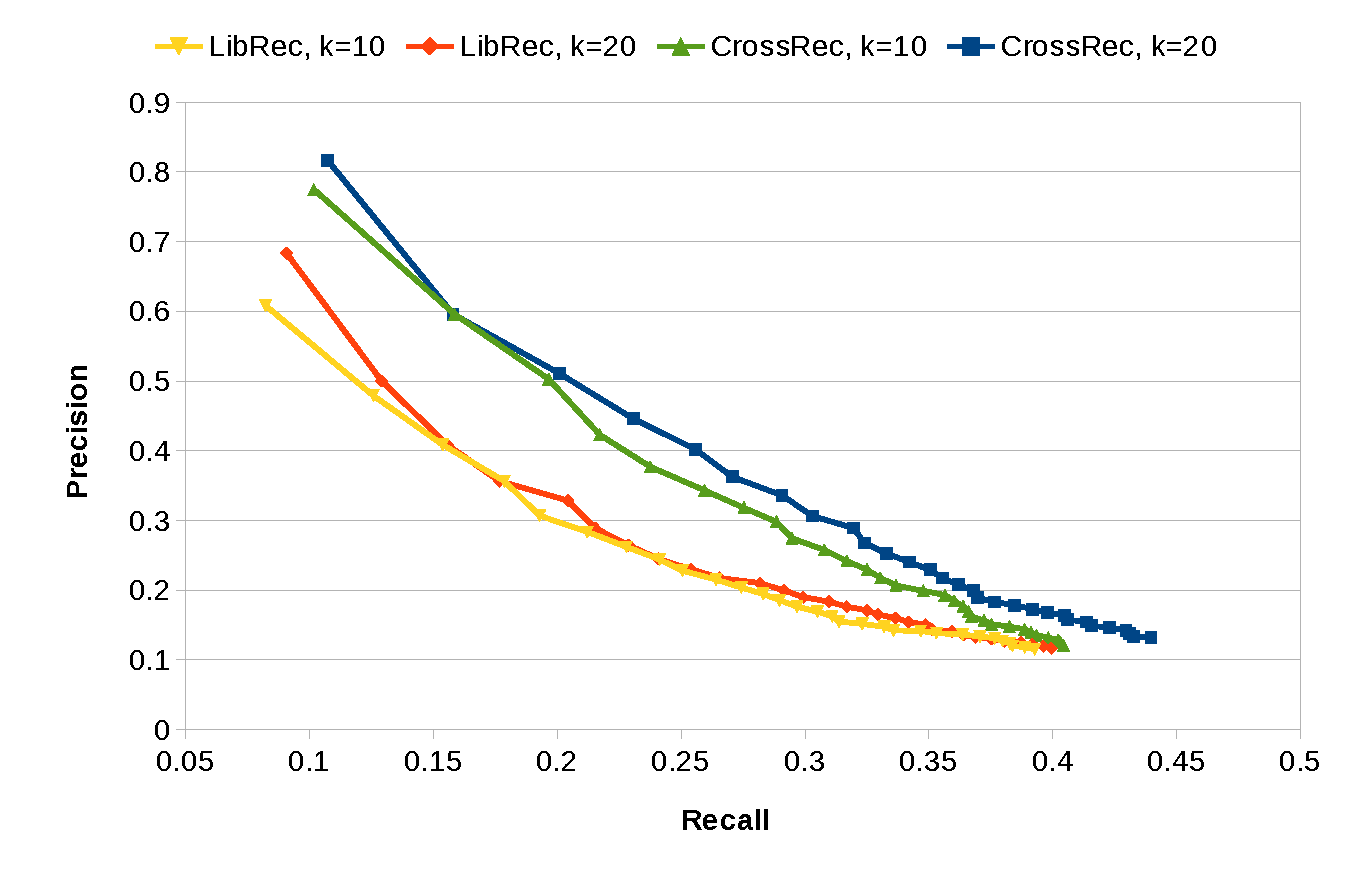
\includegraphics[width=0.45\textwidth]{figs/PrecisionRecall_Fold1.pdf}} & 	
%%		\subfigure[Fold 2]{\label{fig:PrecisionRecallFold2}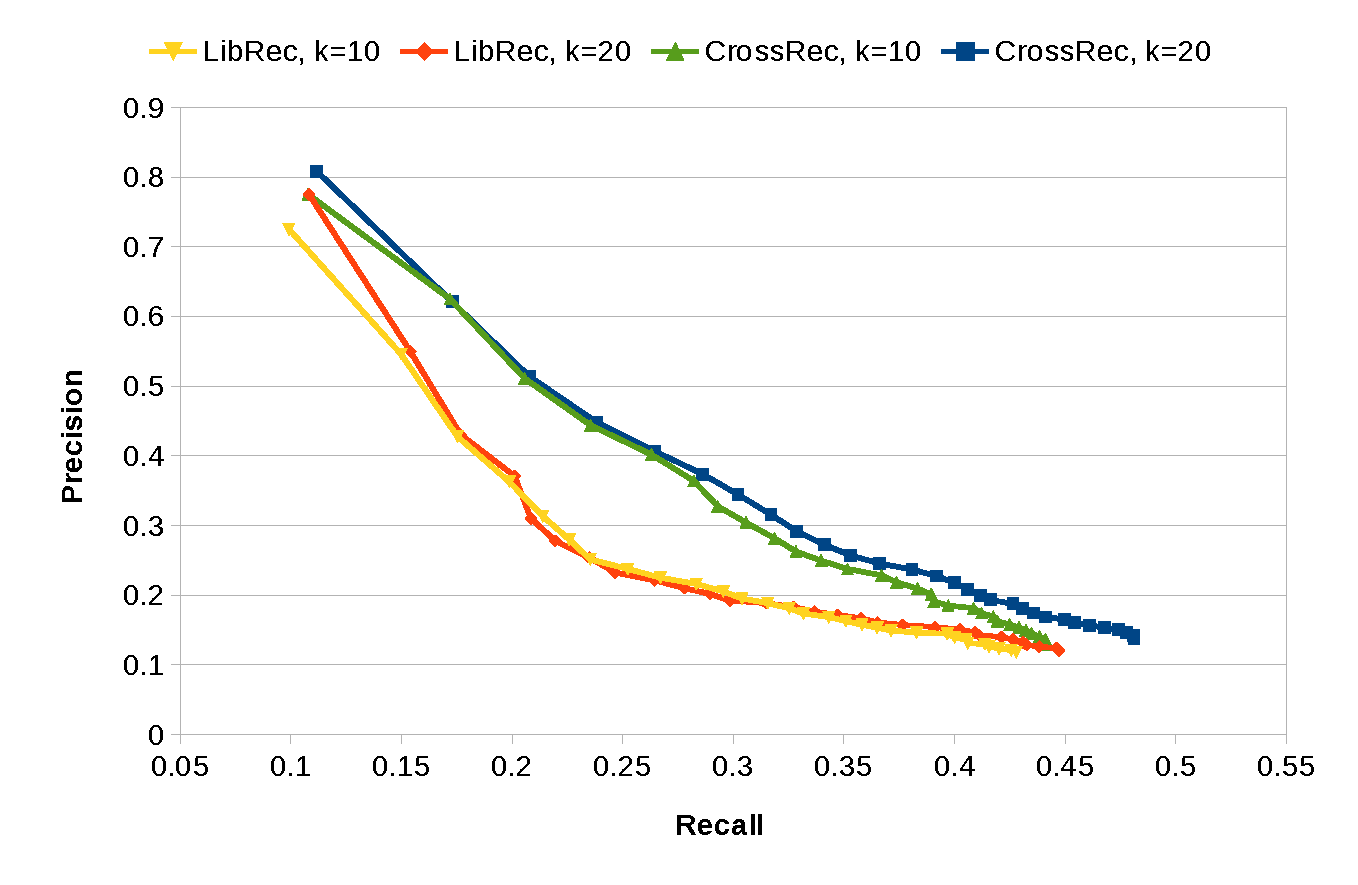
\includegraphics[width=0.45\textwidth]{figs/PrecisionRecall_Fold2.pdf}} \\	
%%		\vspace{-.37cm}	
%%		\subfigure[Fold 3]{\label{fig:PrecisionRecallFold3}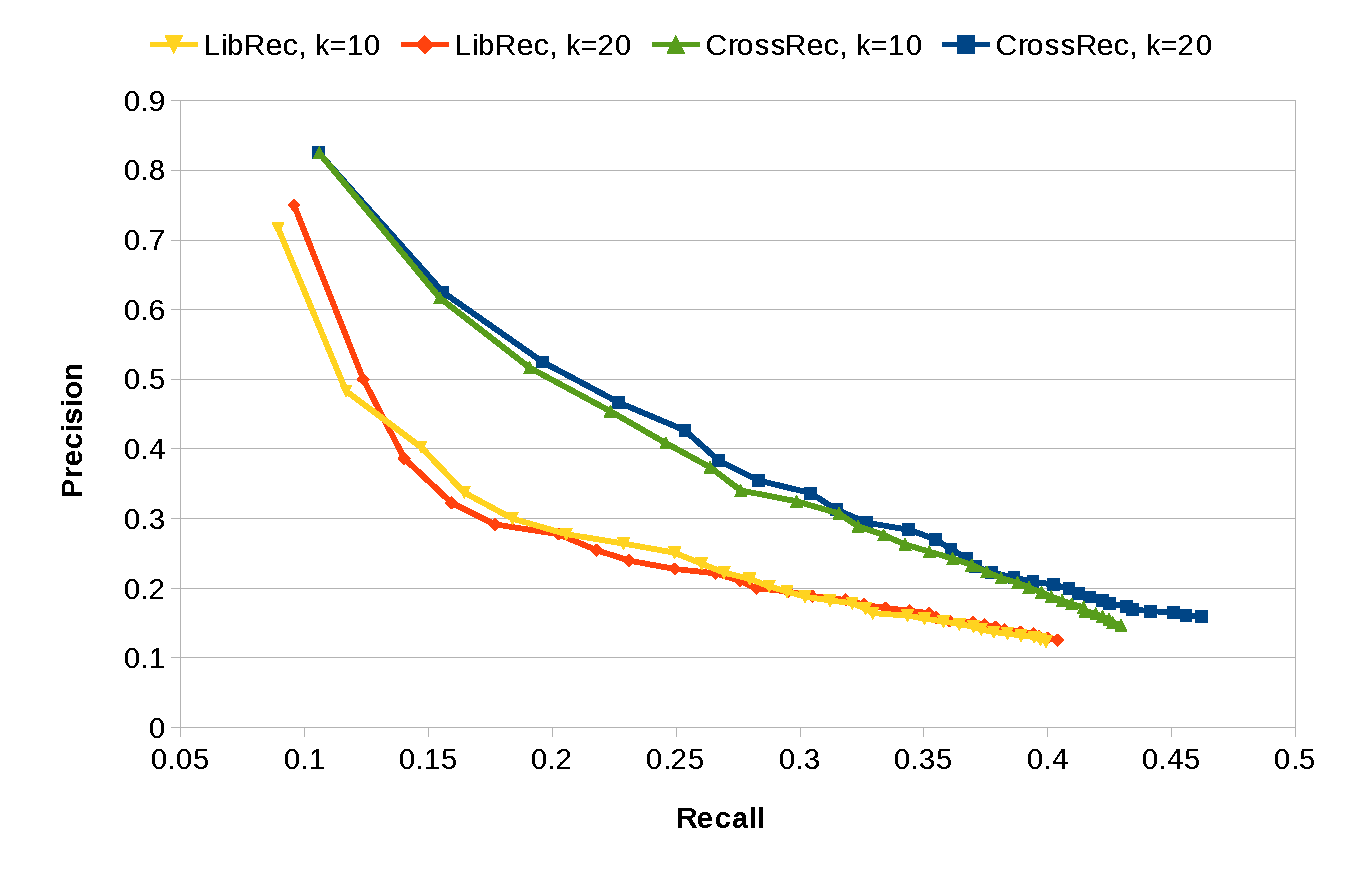
\includegraphics[width=0.45\textwidth]{figs/PrecisionRecall_Fold3.pdf}} & 	
%%		\subfigure[Fold 4]{\label{fig:PrecisionRecallFold4}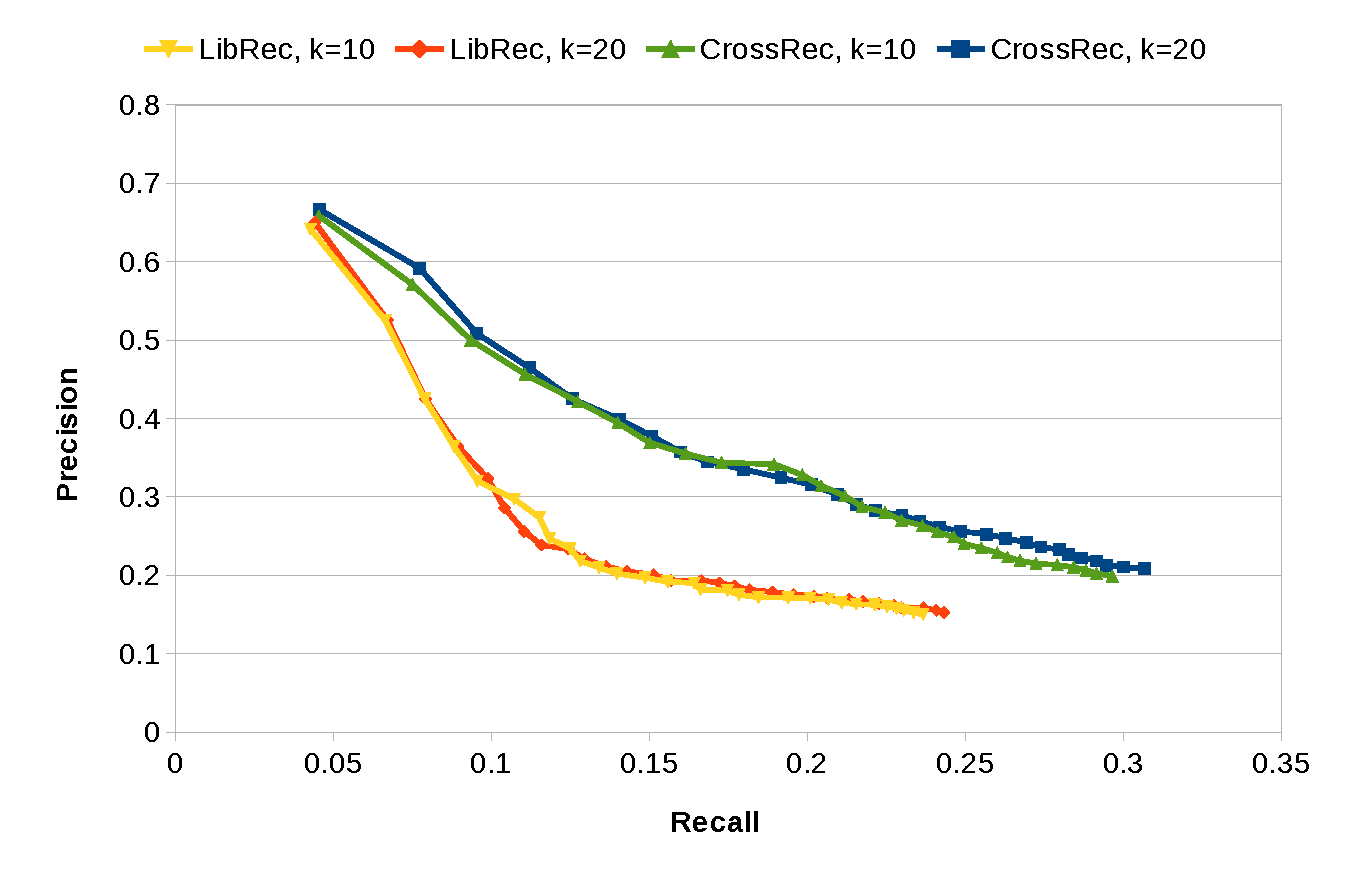
\includegraphics[width=0.45\textwidth]{figs/PrecisionRecall_Fold4.pdf}} \\	
%%		\vspace{-.37cm}	
%%		\subfigure[Fold 5]{\label{fig:PrecisionRecallFold5}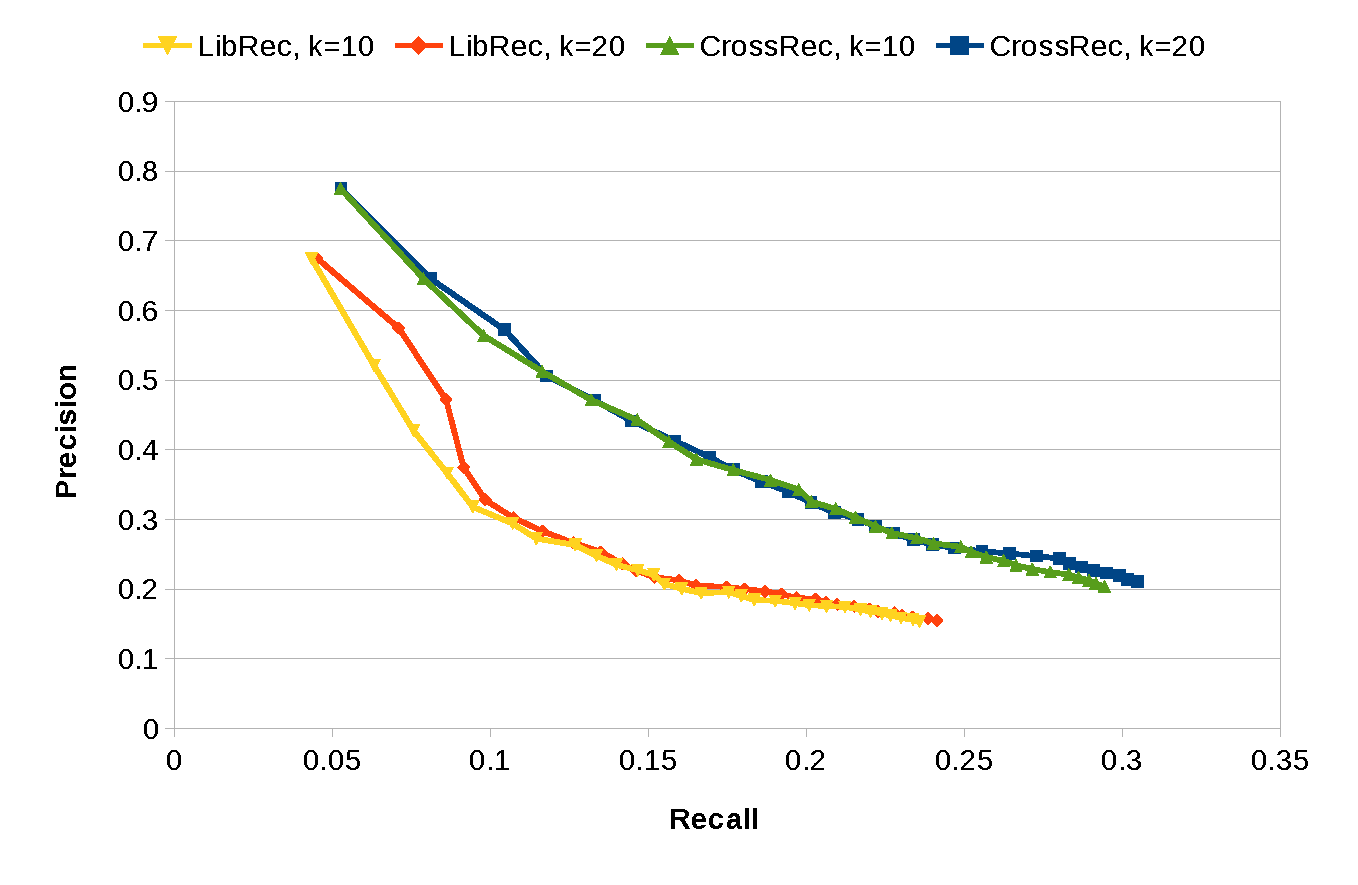
\includegraphics[width=0.45\textwidth]{figs/PrecisionRecall_Fold5.pdf}} & 	
%%		\subfigure[Fold 6]{\label{fig:PrecisionRecallFold6}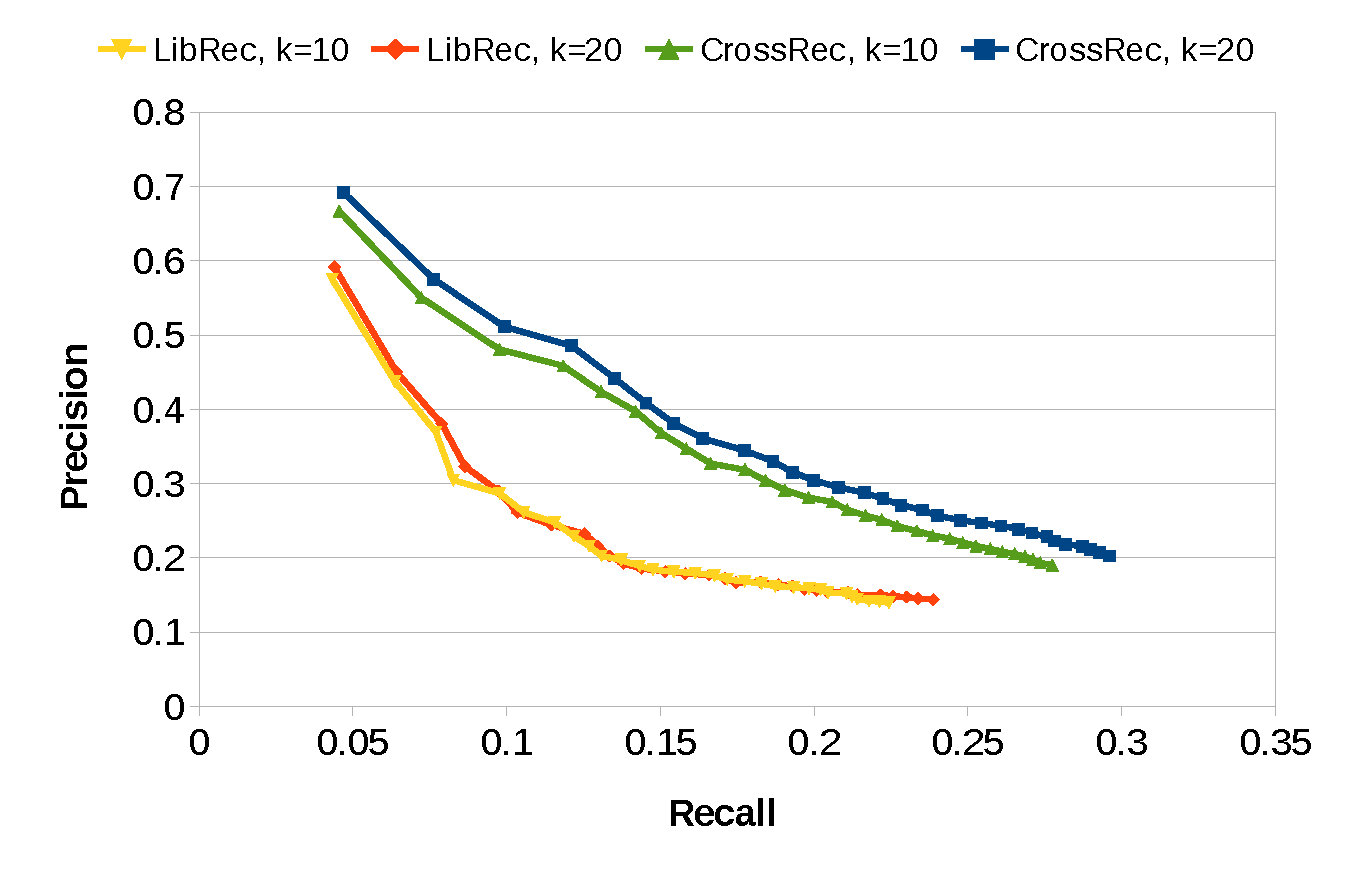
\includegraphics[width=0.45\textwidth]{figs/PrecisionRecall_Fold6.pdf}} \\
%%		\vspace{-.37cm}
%%		\subfigure[Fold 7]{\label{fig:PrecisionRecallFold7}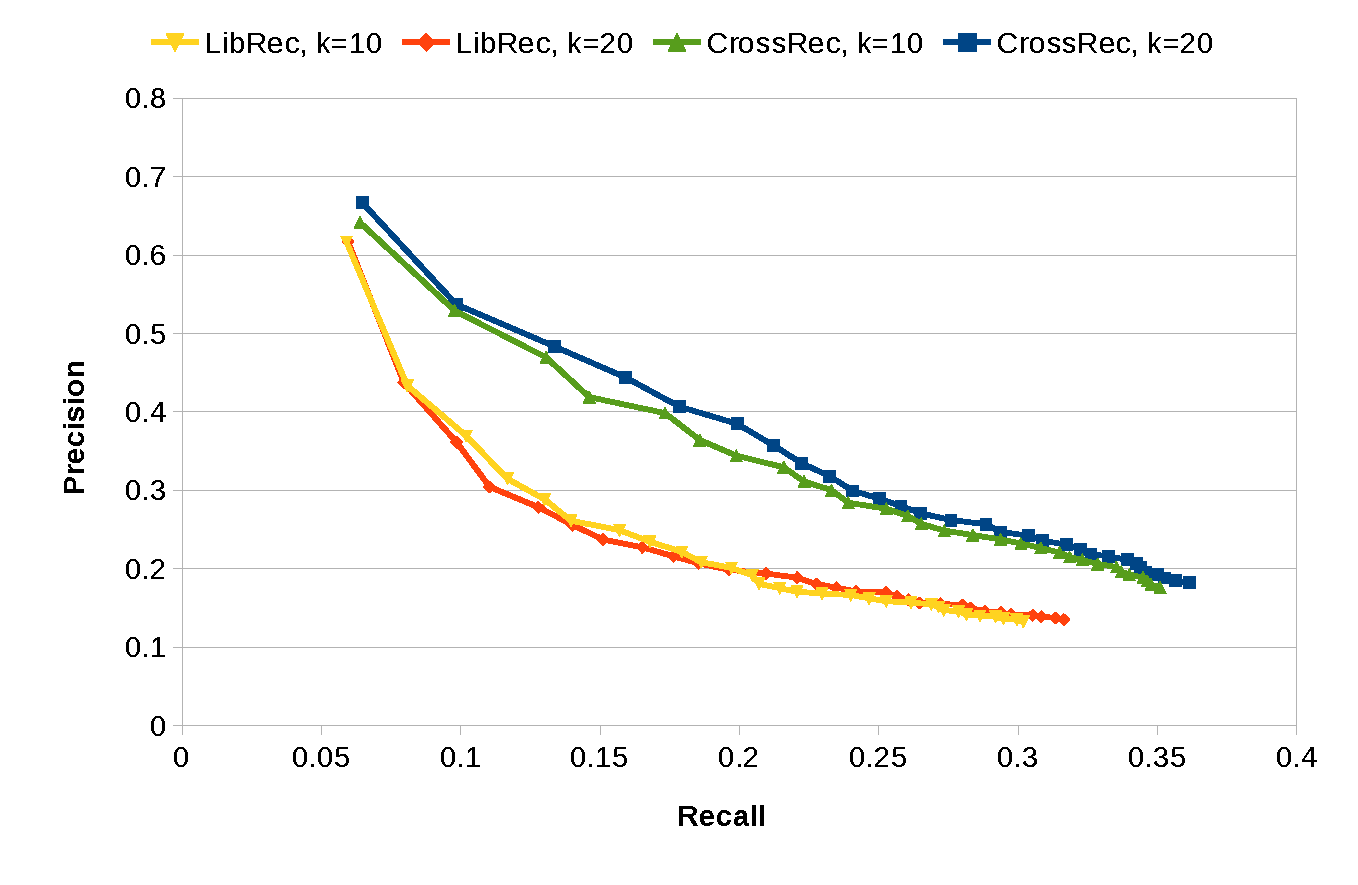
\includegraphics[width=0.45\textwidth]{figs/PrecisionRecall_Fold7.pdf}} & 	
%%		\subfigure[Fold 8]{\label{fig:PrecisionRecallFold8}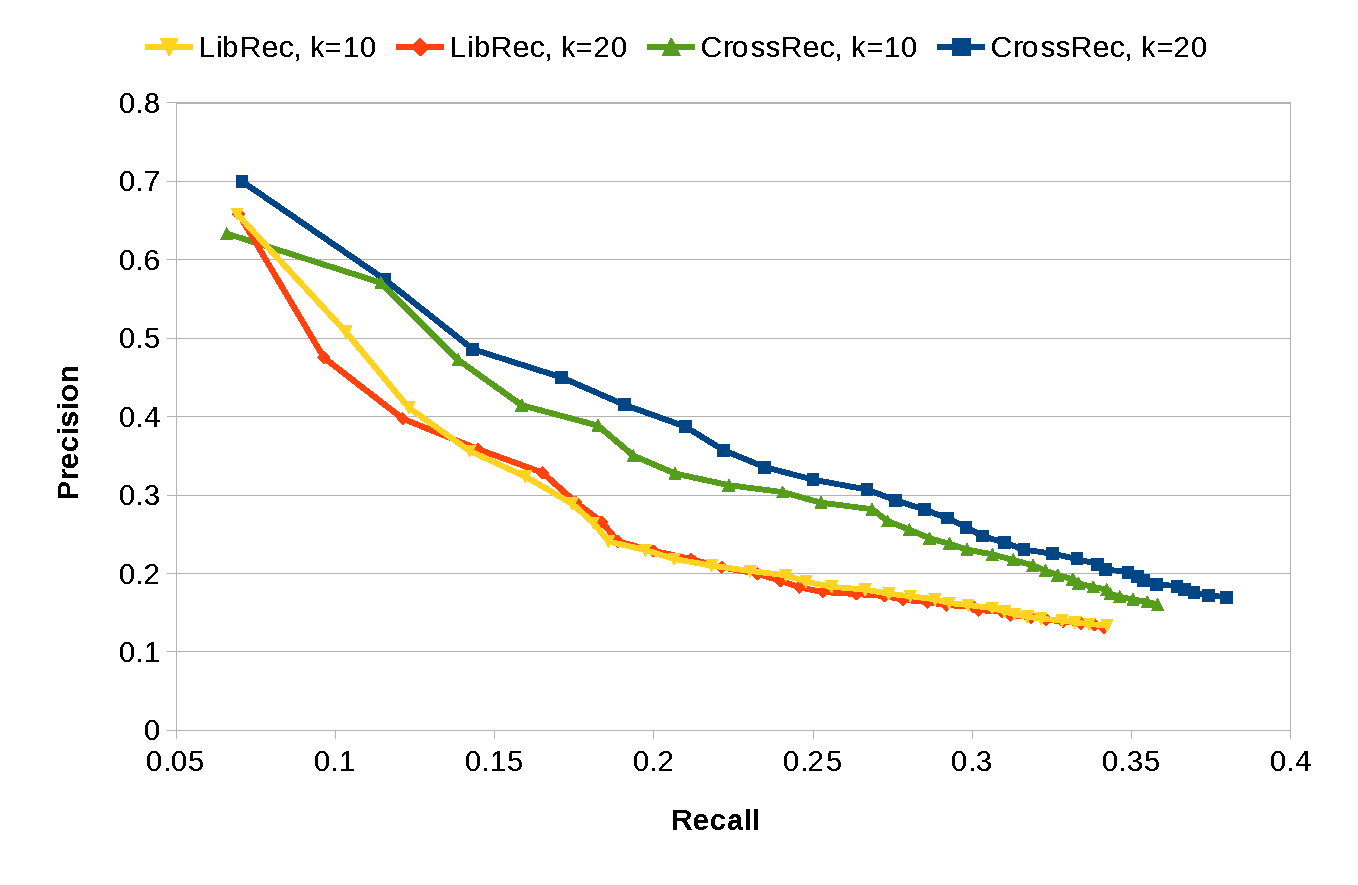
\includegraphics[width=0.45\textwidth]{figs/PrecisionRecall_Fold8.pdf}} \\
%%		\vspace{-.37cm}
%%		\subfigure[Fold 9]{\label{fig:PrecisionRecallFold9}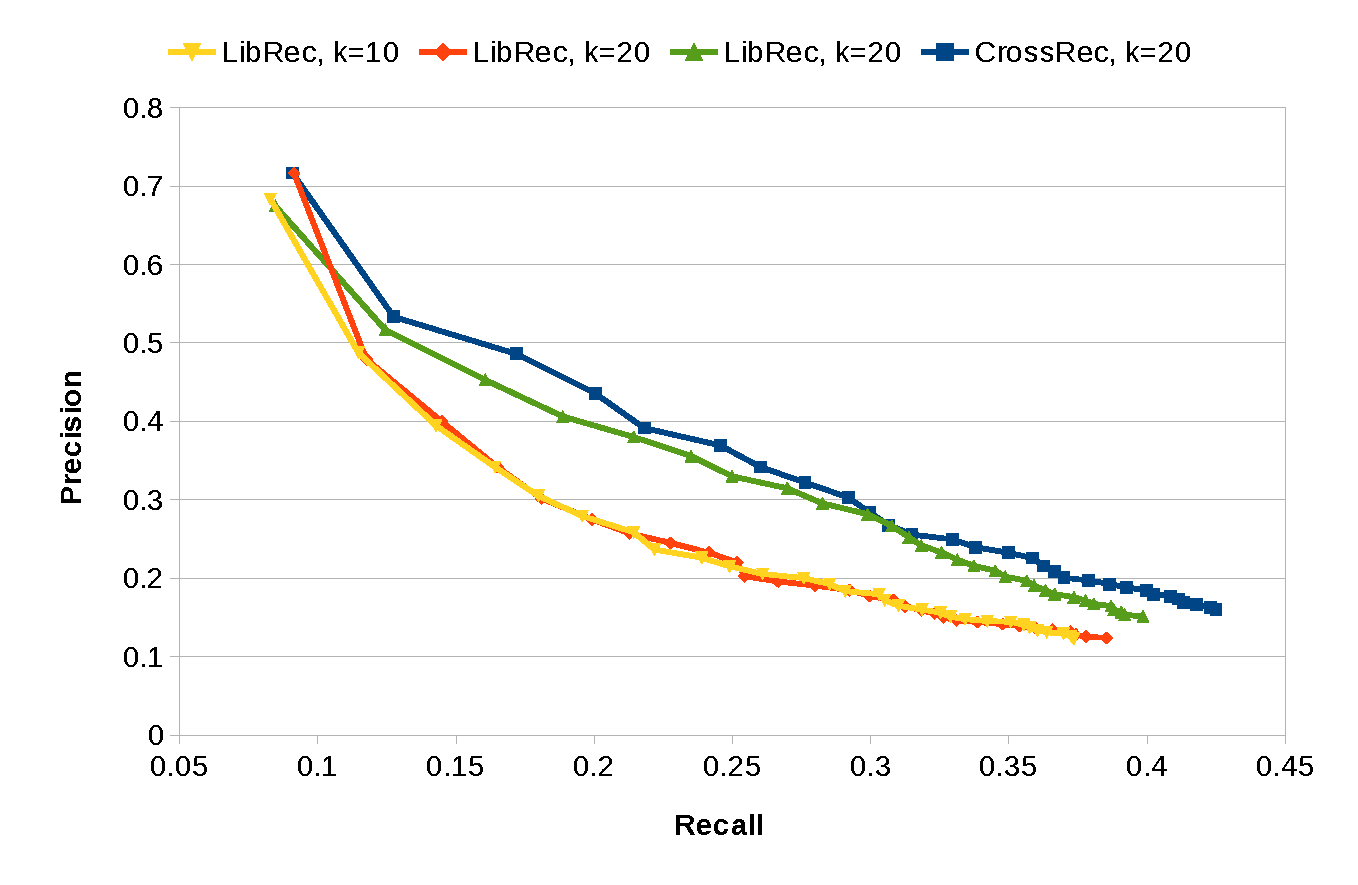
\includegraphics[width=0.45\textwidth]{figs/PrecisionRecall_Fold9.pdf}} & 	
%%		\subfigure[Fold 10]{\label{fig:PrecisionRecallFold10}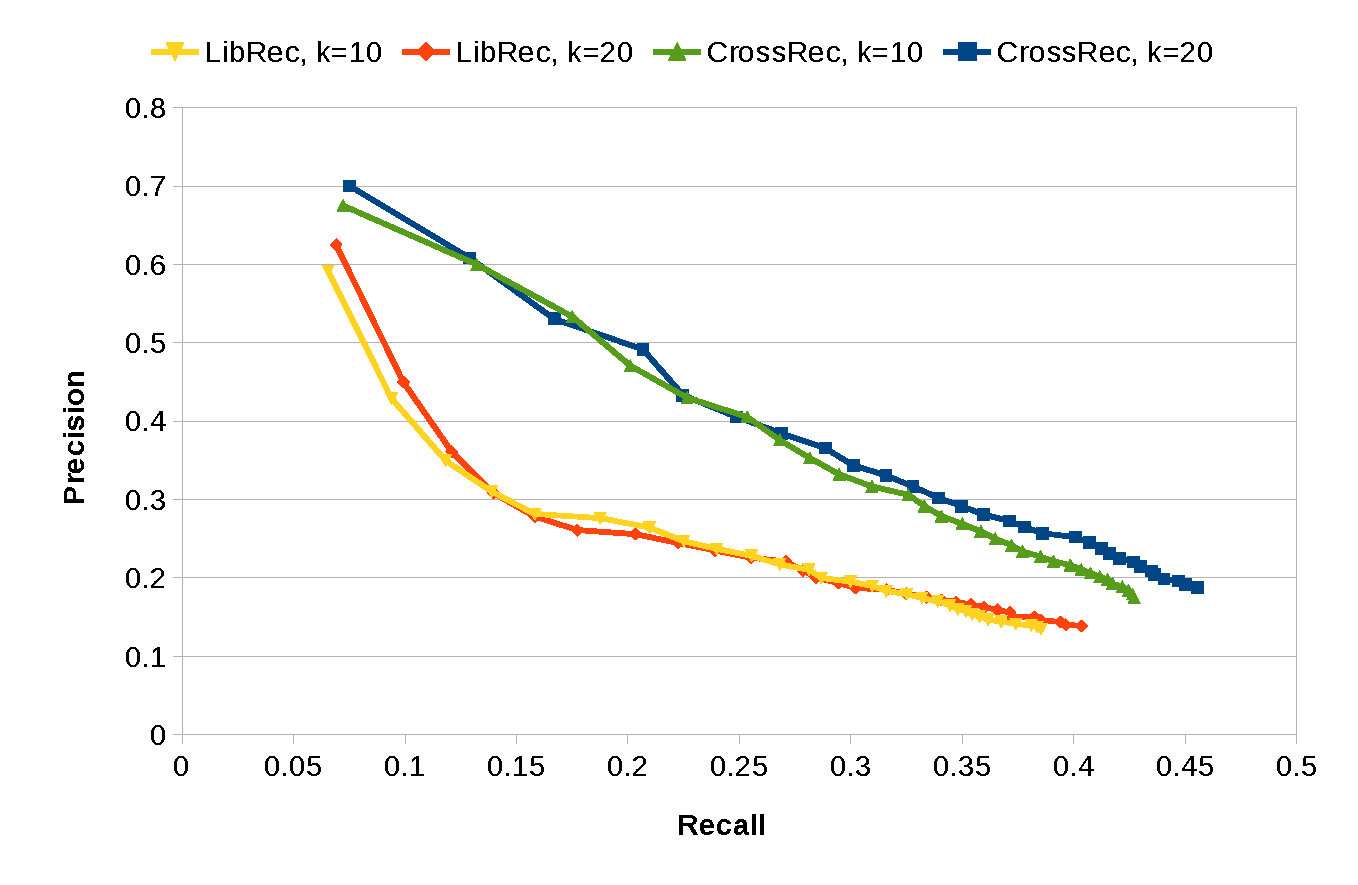
\includegraphics[width=0.45\textwidth]{figs/PrecisionRecall_Fold10.pdf}} \\	
%%	\end{tabular}
%%	\label{fig:PrecisionRecall}	
%%	\caption{\emph{Accuracy: precision@N and recall@N, k=\{10,20\}}}% for \LR and \CR
%%%	\vspace{-.4cm}
%%\end{figure*}
%
%
%
%
%%\vspace{.1cm}
%%%\noindent\textbf{RQ$_1$:} \emph{Does \CR obtain a better success rate compared to \LR?}
%%\noindent \rqsecond
%%\vspace{-.05cm}
%
%
%%
%%\vspace{.1cm}
%%\noindent \revised{\rqsecond}
%%\vspace{-.05cm}
%%
%
%%\begin{table*}[ht]
%%	\footnotesize
%%	\caption{Success rate of \CR on D2 with different number of libraries ($L$).}
%%	\centering
%%%	\begin{tabular}{|r|r|r|r|r|r|r|}\hline
%%	\begin{tabular}{|p{0.7cm}|p{0.7cm}|p{1.0cm}|p{1.0cm}|p{1.0cm}|p{1.0cm}|p{1.0cm}|}\hline
%%		\rowcolor{verylightgray}
%%		\multicolumn{2}{|c|}{} & \multicolumn{5}{c|}{\textbf{Cut-off value (N)}}         \\ \hline%\cline{3-8}
%%%		\rowcolor{verylightgray}
%%		\multicolumn{2}{|c|}{\textbf{Number of libs.}} & 1	 & 3   & 5    & 7   & 10          \\ \hline
%%		{\multirow{2}{*}{$L$}} & 4          & 0.208 & 0.308 & 0.357 & 0.389 & 0.422   \\ \cline{2-7}
%%		& 10         & 0.255 & 0.368 & 0.422 & 0.456 & 0.494   \\ \hline
%%	\end{tabular}
%%	\label{tab:SuccessRate\CRD2}
%%	%\vspace{-.1cm}
%%\end{table*}
%
%\color{black}
%
%
%
%\vspace{.1cm}
%%\textbf{RQ$_2$:} \emph{How well can \LR and \CR recommend third-party libraries in terms of accuracy, sales diversity, and novelty?}
%\noindent \rqsecond
%\vspace{-.05cm}
%
%
%
%
%% $\div$ \ref{fig:PrecisionRecallFold10}
%% \cite{Nguyen:2015:CRV:2942298.2942305}
%
%
%%\LR is highly related to \CR. , we are able to perform a comprehensive evaluation with \LR
%%. 
%%we have access to the source implementation of \LR, thus 
%
%
%
%
%
%
%\noindent%N (the cut-off value for the list of items to be recommended) 
%%\emph{Accuracy:} 
%%We ran both \LR and \CR on \code{D1}. 
%
%\paragraph{\textbf{Accuracy}} To represent accuracy, we vary $N$ from $1$ to $30$ to get \emph{precision@N} and \emph{recall@N}. The rationale behind the selection of $30$ as the maximum cut-off value is that \LR normally produces a short list of recommendations, ranging from $32$ to $50$ items. From the accuracy scores computed using Eq.~\eqref{eqn:Precision} and Eq.~\eqref{eqn:Recall}, the Precision-Recall curves (PRCs) for all $10$ rounds of validation and different values of $k$ were sketched. However, we noticed that the figures representing the folds share a very similar pattern.  Thus, for the sake of clarity, we only show in Fig. \ref{fig:PrecisionRecall} results of the most representative fold. Since a PRC close to the upper right corner represents a better accuracy \cite{DiNoia:2012:LOD:2362499.2362501}, we see that by \LR, changing the number of neighbor $k$ almost makes no difference in its accuracy. Meanwhile for \CR we can notice that an increase of $k$ brings a slightly better accuracy for some testing folds, however the gain is negligible. For all pieces of testing data, \CR always produces a superior accuracy compared to that of \LR.%compared to \LR. %substantially
%
%\begin{figure}[h!]
%	\centering
%	\vspace{-.4cm}
%	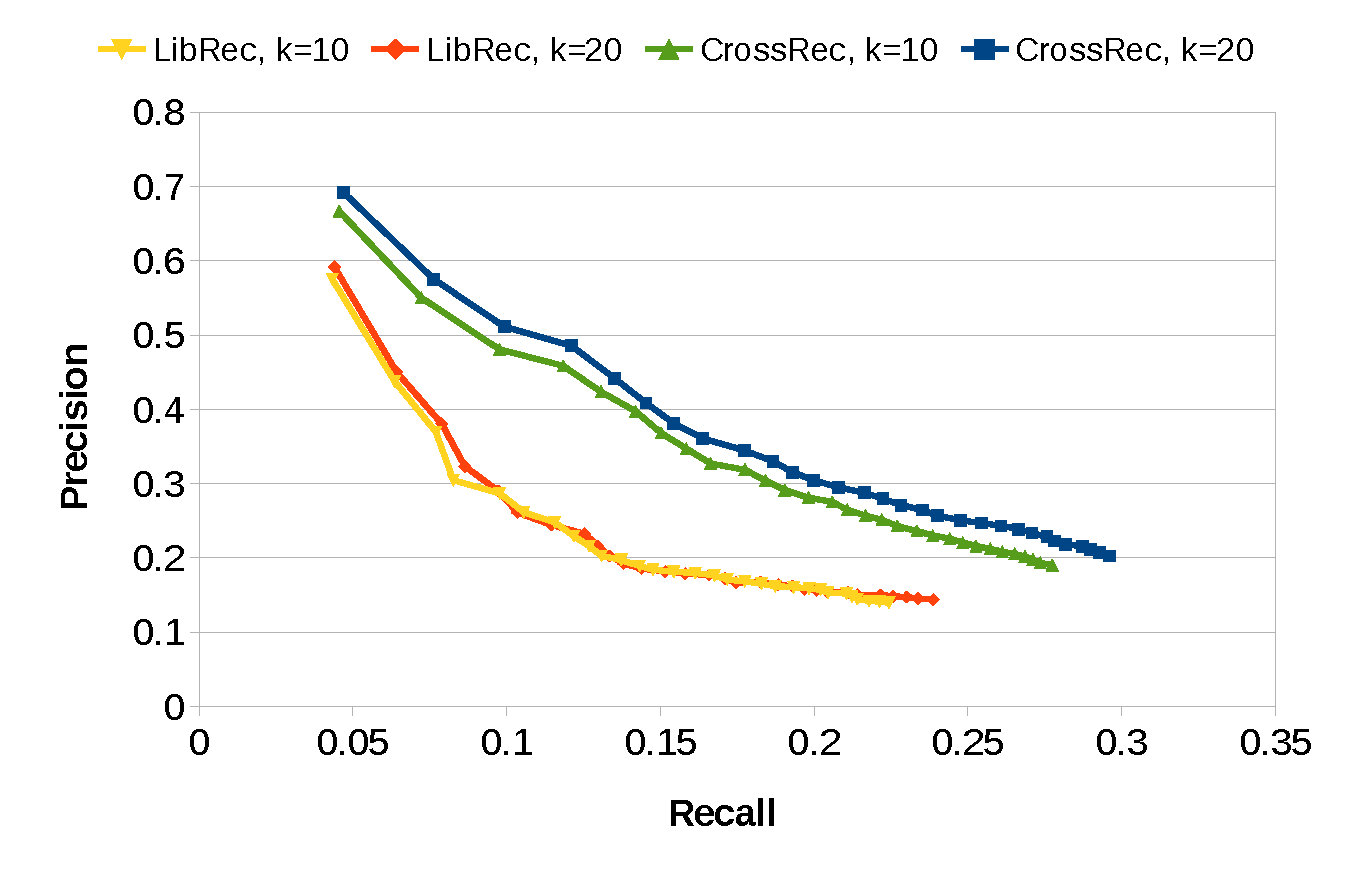
\includegraphics[width=0.86\linewidth]{figs/PrecisionRecall_Fold6.pdf}
%	\vspace{-.7cm}
%	\caption{Precision and Recall.}
%	\label{fig:PrecisionRecall}
%	\vspace{-.5cm}
%\end{figure}
%
%
%
%
%
%
%%\begin{tcolorbox}[boxrule=0.86pt,left=0.3em, right=0.3em,top=0.1em, bottom=0.05em]
%%	\small{In summary, we see that \CR significantly outperforms \LR 
%%		in all considered test configurations concerning \emph{success rate}, with 
%%		a large effect size. The recommendation time for a fold (120 projects) is 
%%		relatively faster for \CR (3s) than for \LR (20s).}
%%\end{tcolorbox}
%
%
%
%
%
%\vspace{.1cm}
%\noindent
%%\emph{Sales Diversity:} 
%\paragraph{\textbf{Sales diversity}} The catalog coverage scores for \LR and \CR are depicted in Table 
%\ref{tab:CatalogCoverage}. The maximum coverage values are $4.594$ and $5.897$ for \LR and 
%\CR, respectively. According to Eq. \eqref{eqn:Coverage}, a higher score means a better 
%coverage. In this sense, the recommendations generated by \CR cover a wider spectrum of 
%libraries than those by \LR for both configurations, \ie $k=10$ and $k=20$, using different 
%cut-off values $N$. Table \ref{tab:Entropy} shows the \emph{entropy} for \LR and \CR. 
%Equation \eqref{eqn:Entropy} suggests that a low entropy value represents a better distribution of 
%items, therefore the recommendations by \CR have a much better distribution than those 
%obtained by \LR. For example, for the case $N=25$ and $k=20$, \CR has an entropy of $0.635$, 
%which is much better than $2.751$, the corresponding value by \LR.
%
%\begin{table}[h!]
%	\footnotesize
%	\caption{Catalog coverage for N=\{5,10,15,20,25\}, k=\{10,20\}.}
%	\centering
%	\begin{tabular}{|p{0.8cm}||p{1.2cm}|p{1.2cm}||p{1.2cm}|p{1.2cm}|} \hline	
%%		\rowcolor{verylightgray}	
%		& \multicolumn{2}{c||}{\textbf{k=10}}  & \multicolumn{2}{c|}{\textbf{k=20}} \\ \hline
%		\textbf{N}	& \LR    & \CR  & \LR    & \CR	  \\ \hline	
%		5       & 0.857   	  & \textbf{1.099}  	& 0.691 		& \textbf{0.814}    \\ \hline
%		10      & 1.760      & \textbf{2.157}  	& 1.346 		& \textbf{1.534}    \\ \hline
%		15      & 2.675      & \textbf{3.278}  	& 1.937 		& \textbf{2.312}    \\ \hline
%		20      & 3.577      & \textbf{4.541}  	& 2.512 		& \textbf{3.143}    \\ \hline
%		25      & 4.594      & \textbf{5.897}  	& 3.139 		& \textbf{4.005}    \\ \hline
%	\end{tabular}
%	\label{tab:CatalogCoverage}
%\end{table}
%
%%According to Table \ref{tab:CatalogCoverage}, increasing the number of neighbours for recommendation adds a decline in coverage for both systems. %Referring to 
%% by this quality indicator, surpasses \LR in the recommendation performance. %gains a better performance compared to that of \LR. 
%% by this quality indicator, 
%
%\begin{table}[h!]
%	\footnotesize
%	\caption{Entropy for N=\{5,10,15,20,25\}, k=\{10,20\}.}
%	\centering
%	\begin{tabular}{|p{0.8cm}||p{1.2cm}|p{1.2cm}||p{1.2cm}|p{1.2cm}|} \hline		
%%		\rowcolor{verylightgray}
%		& \multicolumn{2}{c||}{\textbf{k=10}}  & \multicolumn{2}{c|}{\textbf{k=20}} \\ \hline
%		\textbf{N}	& \LR    & \CR  & \LR    & \CR	  \\ \hline	
%		5       & 0.869   	 & \textbf{0.239}  	& 0.552 		& \textbf{0.127}    \\ \hline
%		10      & 1.752      & \textbf{0.481}  	& 1.098 		& \textbf{0.254}    \\ \hline
%		15      & 2.653      & \textbf{0.723}  	& 1.639 		& \textbf{0.381}    \\ \hline
%		20      & 3.566      & \textbf{0.968}  	& 2.193 		& \textbf{0.508}    \\ \hline
%		25      & 4.500      & \textbf{1.217}  	& 2.751 		& \textbf{0.635}    \\ \hline
%	\end{tabular}
%	\vspace{-.1cm}
%	\label{tab:Entropy}
%\end{table}
%
%
%\noindent
%%\emph{Novelty:} 
%\paragraph{\textbf{Novelty}} The \emph{EPC@N} scores for \LR and \CR are shown in Table~\ref{tab:EPC}. With \LR, changing $k$ from $10$ to $20$ decreases \emph{novelty} for all cut-off values. For example, the \emph{novelty} with $N=25$ and $k=10$ is $0.349$, however once $k$ is changed to $20$, it drops to $0.261$. For \CR, changing the number of neighbours \emph{k} from $10$ to $20$ does not bring a rise in \emph{novelty}. As shown in Table~\ref{tab:EPC}, \CR always obtains scores that are higher than those of \LR. For example, when $N=5$ and $k=20$, \CR achieves a value of $0.292$ for \emph{novelty}, whereas \LR gets $0.114$. This, together with the example in Section~\ref{sec:Example}, confirms that \CR recommends libraries that are closer to the long tail than \LR can do.  %with respect to \emph{Novelty} 
%%\vspace{-.2cm}
%
%\begin{table}[t]
%	\footnotesize
%	\caption{EPC for N=\{5,10,15,20,25\}, k=\{10,20\}.}
%	\centering
%	\begin{tabular}{|p{0.8cm}||p{1.2cm}|p{1.2cm}||p{1.2cm}|p{1.2cm}|} \hline	
%%		\rowcolor{gray}	
%		& \multicolumn{2}{c||}{\textbf{k=10}}  & \multicolumn{2}{c|}{\textbf{k=20}} \\ \hline
%		\textbf{N}	& \LR    & \CR  & \LR    & \CR	  \\ \hline	
%		5       & 0.187	   	 & \textbf{0.291}  	& 0.114	 		& \textbf{0.292}    \\ \hline
%		10      & 0.264      & \textbf{0.349}  	& 0.166  		& \textbf{0.344}    \\ \hline
%		15      & 0.296      & \textbf{0.376}  	& 0.204 		& \textbf{0.377}    \\ \hline
%		20      & 0.320      & \textbf{0.391}  	& 0.236 		& \textbf{0.399}    \\ \hline
%		25      & 0.349      & \textbf{0.401}  	& 0.261 		& \textbf{0.416}    \\ \hline
%	\end{tabular}
%	\label{tab:EPC}
%\end{table}
%
%
%
%\begin{table*}[h!]
%	\footnotesize
%	\caption{Wilcoxon rank sum test adjusted $p$-values for N=\{3,5,10,15\}, 
%		k=10.}
%	\centering
%	\begin{tabular}{|p{0.8cm}||p{1.2cm}|p{1.2cm}||p{1.2cm}|p{1.2cm}||p{1.2cm}|} \hline	
%		%	\begin{tabular}{|r||r|r||r|r||r|}\hline
%%		\rowcolor{gray}
%		& \multicolumn{2}{c||}{\textbf{Accuracy}} &  \multicolumn{2}{c||}{\textbf{Sales Diversity}}   & \textbf{Novelty}  \\ \hline
%		\textbf{N} & Precision  &  Recall   & Coverage   & 	Entropy  & EPC \\\hline
%		3          & 1.58e-16&5.41e-08 & 0.0005 & 6.50e-05& 4.33e-05 \\\hline
%		5          & 1.35e-24& 9.10e-12 & 0.001 & 6.50e-05& 4.33e-05 \\\hline
%		10         & 1.07e-21& 9.12e-12 & 0.003& 4.33e-05& 1.52e-04 \\\hline
%		15         &  1.10e-14 & -- & 0.003& 6.50e-05& 2.06e-04 \\\hline
%	\end{tabular}
%	\label{tab:Wilcoxon}
%\end{table*}
%%
%
%
%\begin{table*}[h!]
%	\footnotesize
%	\caption{Cliff's $d$ results for N=\{3,5,10,15\}, k=10. Labels in parenthesis indicate the magnitude (n:negligible, s:small, l:large).}
%	\centering
%	\begin{tabular}{|p{0.8cm}||p{1.2cm}|p{1.2cm}||p{1.2cm}|p{1.2cm}||p{1.2cm}|} \hline	
%		%	\begin{tabular}{|r||r|r||r|r||r|}\hline
%%		\rowcolor{gray}
%		& \multicolumn{2}{c||}{\textbf{Accuracy}} &  \multicolumn{2}{c||}{\textbf{Sales Diversity}}   & \textbf{Novelty}  \\ \hline
%		\textbf{N} & Precision & Recall  & Coverage & Entropy & EPC  \\ \hline
%		3          &  0.18 (s) & 0.12 (n)& 0.92 (l)& 0.96 (l)& 1.00 (l) \\ \hline
%		5          &  0.23 (s) & 0.16 (s)& 0.86 (l)&  0.98 (l)& 1.00 (l) \\ \hline
%		10         &  0.22 (s) & 0.16 (s)& 0.80 (l)&  1.00 (l)& 0.94 (l) \\ \hline
%		15         &  0.17 (s) & -- & 0.80 (l)&  0.98 (l) & 0.90 (l)\\ \hline
%	\end{tabular}
%	\label{tab:Cliff}
%	%\vspace{-.1cm}
%\end{table*}
%
%
%
%%====================old tables are here========================================
%%===============================================================================
%%\begin{table*}[h!]
%%	\footnotesize
%%	\caption{Wilcoxon rank sum test adjusted $p$-values for N=\{3,5,10,15\}, 
%%		k=10.}
%%	\centering
%%	\begin{tabular}{|r|r|r|r|r|r|r|}
%%		\hline
%%		\rowcolor{verylightgray}
%%		& \textbf{Success Rate} &     
%%		\multicolumn{2}{c|}{\textbf{Accuracy}}      &   
%%		\multicolumn{2}{c|}{\textbf{Sales Diversity}}   & \textbf{Novelty}      
%%		\\ \hline
%%		\textbf{N} & Success Rate          & Precision               & 
%%		Recall                & Coverage                  & 
%%		Entropy               & EPC                   \\ \hline
%%		3          & 0.02& 1.58e-16&5.41e-08 & 0.0005 & 6.50e-05& 4.33e-05\\ 
%%		\hline
%%		5          & 0.02& 1.35e-24& 9.10e-12 & 0.001 & 6.50e-05& 4.33e-05\\ 
%%		\hline
%%		10          & 0.17& 1.07e-21& 9.12e-12 & 0.003& 4.33e-05& 1.52e-04\\ 
%%		\hline
%%		15          & 0.002&  1.10e-14 & -- & 0.003& 6.50e-05& 2.06e-04\\ \hline
%%	\end{tabular}
%%	\label{tab:Wilcoxon}
%%\end{table*}
%%%
%%\begin{table*}[ht]
%%	\footnotesize
%%	\caption{Cliff's $d$ results for N=\{3,5,10,15\}, k=10. Labels in parenthesis indicate the magnitude (n:negligible, s:small, l:large).}
%%	\centering
%%	\begin{tabular}{|r|r|r|r|r|r|r|}\hline
%%		\rowcolor{verylightgray}
%%		& \textbf{Success Rate} &     \multicolumn{2}{c|}{\textbf{Accuracy}}      &   \multicolumn{2}{c|}{\textbf{Sales Diversity}}   & \textbf{Novelty}      \\ \hline
%%		\textbf{N} & Success Rate          & Precision               & Recall                & Coverage                  & Entropy               & EPC                   \\ \hline
%%		3          & 0.70 (l)& 0.18 (s)& 0.12 (n)& 0.92 (l)& 0.96 (l)& 1.00 (l) \\ \hline
%%		5          & 0.74 (l)&  0.23 (s)& 0.16 (s)& 0.86 (l)&  0.98 (l)& 1.00 (l) \\ \hline
%%		10         & 0.93 (l)&  0.22 (s)& 0.16 (s)& 0.80 (l)&  1.00 (l)& 0.94 (l) \\ \hline
%%		15         & 0.58 (l)&  0.17 (s)& -- & 0.80 (l)&  0.98 (l) & 0.90 (l)\\ \hline
%%	\end{tabular}
%%	\label{tab:Cliff}
%%	%\vspace{-.1cm}
%%\end{table*}
%%===============================================================================
%
%
%
%Also in this case (see columns 2-6 of Tables \ref{tab:Wilcoxon} and \ref{tab:Cliff}), our analyses are supported by statistical procedures. Differences are always statistically significant. The effect size is negligible/small for \emph{accuracy} (precision and recall), whereas it is large for all other indicators \emph{sales diversity} and \emph{novelty}.
%
%
%
%\begin{tcolorbox}[boxrule=0.86pt,left=0.3em, right=0.3em,top=0.1em, bottom=0.05em]
%	\small{The results in Fig.~\ref{fig:PrecisionRecall} and 
%		Tables~\ref{tab:CatalogCoverage},~\ref{tab:Entropy},~\ref{tab:EPC} demonstrate 
%		that \CR significantly outperforms \LR concerning 
%		\emph{accuracy}, \emph{sales diversity}, and \emph{novelty}, with a 
%		small/negligible effect size for \emph{accuracy} and large elsewhere.}
%\end{tcolorbox}
%
%%. Furthermore, \CR significantly outperforms 
%
%%\begin{tcolorbox}[boxrule=0.86pt,left=0.3em, right=0.3em,top=0.1em, bottom=0.05em]
%%%	\color{blue}
%%	\revised{\small{%The results in Fig.~\ref{fig:PrecisionRecall} and Tables~\ref{tab:CatalogCoverage},~\ref{tab:Entropy},~\ref{tab:EPC} 	
%%	Altogether, we see that \CR significantly outperforms \LR in all considered test configurations concerning \emph{success rate}, with a large effect size, and concerning \emph{accuracy}, \emph{sales diversity}, and \emph{novelty}, with a small/negligible effect size for \emph{accuracy} and large elsewhere. The recommendation time for a fold (120 projects) is relatively faster for \CR (3s) than for \LR (20s).}}
%%	\color{black}
%%\end{tcolorbox}
%
%
%
%%\vspace{.2cm}
%%\textbf{RQ$_3$:} \emph{Is the performance difference between the two systems statistically significant?}
%%\vspace{.1cm}
%%
%%To see if the improvement of the proposed approach is statistically significant and substantial, we perform a Wilcoxon rank sum test \cite{Wilcoxon1992} on all the quality scores for both systems, using $k=10$ and $N=\{3,5,10,15\}$. The $p$-values for all quality metrics are shown in Table~\ref{tab:Wilcoxon}. The null hypothesis is that there are no differences between the performance of \CR and that of \LR. Using $5\%$ as the confidence level, we see that by all quality indicators the \emph{p-values} are always lower than $5 \times e^{-2}$. Cliff's $d$ values are reported in Table \ref{tab:Cliff}. As the table shows, the observed differences are always in favor of \CR (\ie effect sizes are always positive). Magnitude of the computed Cliff's $d$ is small for precision and recall, while it is large for all other indicators, including Success Rate.
%%
%%\begin{tcolorbox}
%%In this sense, we reject the null hypothesis and conclude that the performance improvement obtained by \CR is statistically significant. %or \emph{p-value} $< 5 \times e^{-2}$ . in terms of all quality metrics. 
%%\end{tcolorbox}
%
%\vspace{.1cm}
%%\textbf{RQ$_3$:} \emph{What are the reasons for the performance difference?}
%\noindent \rqthird
%\vspace{-.05cm}
%
%%Last but not least, w
%%\PN{The explanation has been substantially improved compared to the old version}
%We attempt to ascertain why \CR outperforms \LR. This task might necessitate further investigations, both 
%qualitative and quantitative research. However, by carefully studying the internal design of \LR, we found out that 
%the improvement attributes to the following facts. In the first place, \CR employs a completely different approach 
%to represent projects and libraries: it encodes the relationships among them into a graph. Second, to compute the 
%similarity between two projects, \CR assigns a weight to every library node using tf-idf (see 
%Eq.~\eqref{eqn:TFIDF}). In this way, the level of importance of a node is disproportional to its popularity. This is 
%similar to the context of document matching where popular terms are given a low weight 
%\cite{DBLP:journals/ijswis/HliaoutakisVVPM06}. For instance, in Fig.~\ref{fig:Graph}, $lib_1$ is a popular node since 
%it is referred by $4$ projects and this makes it have a low weight. As a result, \CR is able to better capture the 
%similarity between two projects compared to \LR, which equally treats all libraries. Third, \LR employs a very 
%simple collaborative-filtering technique, though it also considers a set of k-nearest neighbor similar projects for 
%finding libraries, it neglects their similarity level by considering all projects in the same way.~Also, the technique 
%assigns more weight to popular libraries without considering the degree of similarity between projects, from where the 
%libraries come. This explains why \LR recommends very popular items as shown in Section~\ref{sec:Example}.~In 
%contrast, \CR improves by assigning a larger weight to libraries that come from highly similar projects (see 
%Eq.~\eqref{eqn:Prediction}). In other words, given a project, \CR is able to ``mimic'' the behavior of highly 
%similar projects, it attempts to suggest a comparable set of libraries. Lastly, \LR exploits association rule mining 
%which indeed mines items that co-exist. This is why the coverage of the recommended items is low compared to what 
%achieved by \CR.
%
%\begin{tcolorbox}[boxrule=0.86pt,left=0.3em, right=0.3em,top=0.1em, bottom=0.05em]
%	\small{Our qualitative analysis suggests that the improvements achieved by 
%		\CR with respect to \LR are due to the weighting scheme being 
%		applied, which also considers the projects' similarity, \ie it rewards 
%		recommendation of libraries from similar projects.}
%	%Altogether, we see that the improvement by \CR is obtained thanks to the weighting scheme applied to both libraries and projects. With \CR, the collaborative-filtering technique is well practiced in the sense that highly similar projects are more preferred to be mined. Meanwhile, \LR employs a na\"ive collaborative-filtering technique, which ignores the degree of similarities among projects by treating them equally. As a result, the libraries recommended by \CR are more relevant, even though they are not popular. %Furthermore, since \LR prefers high frequency libraries, which decreases novelty. 
%\end{tcolorbox}
%%\vspace{-.2cm}
%
%%The association rule mining module also contributes to 
%
%
%
%
%%\color{blue}
%
%\vspace{.1cm}
%\noindent \revised{\rqfourth}
%\vspace{-.05cm}
%
%
%%amount of data used as query. ratio of 
%% as the ratio of query to testing data
%\revised{Finally, we studied whether an increase in the input data contributes to an improvement in the performance of \CR. As it was already mentioned in Section~\ref{sec:ResearchQuestions}, $r$ is the ratio of libraries used as query over the total number of libraries that a project contains. For this evaluation, rather than using $r=50\%$, we varied it along the following values: $20\%$, $40\%$, $60\%$, and $80\%$, and measured the achieved level of performance. This simulates different levels of a project's maturity: at the beginning when the developer has just included a small number of libraries, or later on when more libraries have been accumulatively populated alongside the project's lifecycle. This research question aims at studying if \CR can assist the developer in choosing the right libraries at different stages of the development process.}
%
%
%\begin{figure}[h!]
%	%	\color{blue}
%	\centering
%	%	\vspace{-.4cm}
%	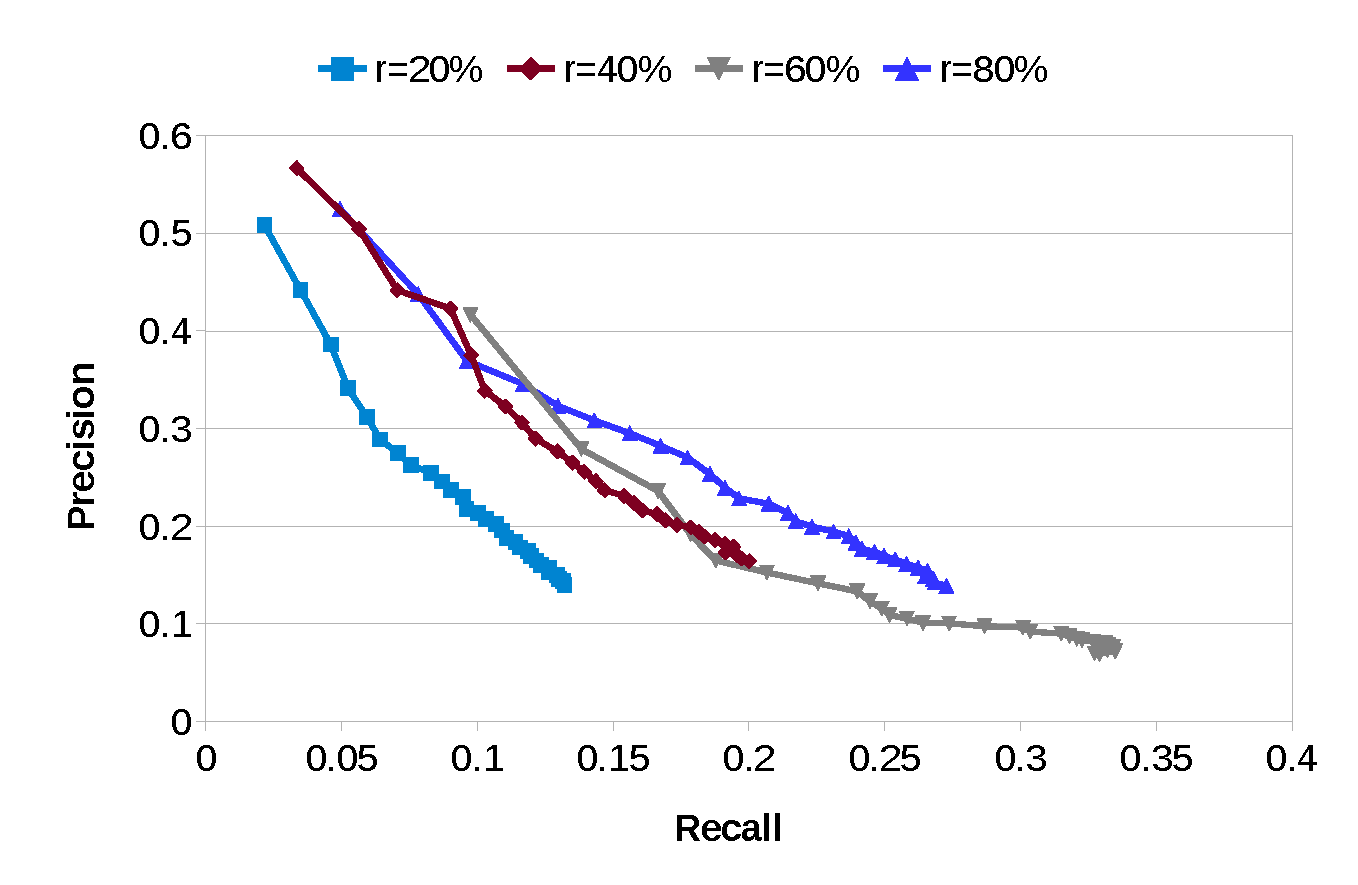
\includegraphics[width=0.86\linewidth]{figs/PrecisionRecall_QueryGroundTruth.pdf}
%	%	\vspace{-.7cm}
%	\caption{\revised{Precision and recall for different amounts of testing and ground-truth data.}}
%	\label{fig:PrecisionRecall_QueryGroundTruth}
%	%	\vspace{-.5cm}
%\end{figure}
%
%%As a PRC close to the upper right corner corresponds to 
%%However, the tendency tends to stagnate when $r$ becomes larger. 
%
%\revised{Fig.~\ref{fig:PrecisionRecall_QueryGroundTruth} reports the precision and recall curves (PRCs) obtained by the configurations. As a better accuracy is represented by a PRC close to the upper right corner~\cite{DiNoia:2012:LOD:2362499.2362501},\cite{Davis:2006:RPR:1143844.1143874}, we see that generally there is an improvement in the recommendation performance when $r$ increases. In particular, there is a sharp growth in precision and recall when $r$ is changed from $20\%$ to $40\%$. However, the gain tends to stagnate when $r$ becomes larger. For instance, the change in performance between $r=40\%$ and $r=60\%$ is small and can be considered as negligible. Similarly, when $r$ goes up to $80\%$ from $60\%$, there is also a marginal change in accuracy. This corresponds to a saturation: at a certain threshold of $r$, \eg $r=50\%$ or $r=60\%$, a little or almost no performance gain can be obtained. In essence, that means \CR can achieve a decent level of accuracy once the developer has included around a half of the total number of libraries.}
%
%
%
%\begin{tcolorbox}[boxrule=0.86pt,left=0.3em, right=0.3em] %,top=0.1em, bottom=0.05em
%	%	\color{blue}
%	\revised{\small{For \CR, an increase in the amount of input data considerably improves the overall performance when the ratio of query to testing data $r$ is small. However, such the gain is disproportionate to $r$.}}
%\end{tcolorbox}
%
%\color{black}
%
%
%\subsection{Threats to Validity} \label{sec:ThreatsToValidity}
%
%We identify the threats that may adversely affect the validity of the experiments as well as the countermeasures taken to mitigate them. %In particular, we focus on internal andexternal threats to validity as discussed below.
%
%\noindent\textit{Threats to internal validity}  are related to any factors internal to our study that can influence our results. 
%%In the performed experiments, we did not consider the version number of project libraries. Even though this is a limitation of the current implementation of \CR, also \LR neglects library versions and consequently the performance comparison between the two systems has not been affected.
%The performances achieved by \CR can depend on the values of $N$ and $k$. We showed in the paper results for $k=10, 20$, and for $N=5, 10, 15, 20, 25$ (see more in Section \ref{sec:Discussions}). Results for other values of $N$ and $k$ are consistent with what we already found.
%
%\revised{The comparison with \LF and \LC has been done in an indirect manner through their corresponding datasets, and this might possibly pose a threat to internal validity. We attempted to mitigate such a threat by exploiting the same experimental settings as well as performing various trials on the same datasets. All the additional experiments yielded comparable outcomes to those presented in the paper.}
%
%
%%By the evaluation, besides the main experiments, we conducted additional trials 
%%using various combinations of $N$ and $k$ to further validate the outcomes. All 
%%the additional experiments produced comparable outcomes to those presented in 
%%the paper.
%
%%As we explained in Section \ref{sec:\CR}, \CR recommends libraries and not specific library versions. It is possible that in a specific context a given library version might be more relevant than another, or even than a different library. We plan to investigate with this specific limitation in our future work.
%
%\noindent\textit{Threats to external validity} concern the 
%generalizability of our findings. In the data collection phase, we tried to 
%cover a wide range of possibilities by mitigating also the fact that  many 
%repositories in GitHub are of low quality, which is especially true when they 
%do not have many stars. The set of  $1,200$ GitHub projects was 
%randomly created by obtaining the following distribution of stars: 14 projects 
%have 0 stars, 135 projects have $[$1-4$]$ stars, 66 projects have $[$5-9$]$ 
%stars, 512 projects have $[$10-99$]$ stars, 300 projects have $[$100-499$]$ 
%stars, 78 projects have $[$500-999$]$ stars, and 95 projects have more than 
%1,000 stars. Moreover, the number of libraries that a project in the considered dataset 
%includes varies considerably from $10$ to more than $500$. 
%
%
%%They are related to the experimental settings presented in the paper, concerning the simulated setting used to evaluate the tool. 
%%
%
%\noindent\textit{Threats to construct validity} are whether the setup and measurement in the study reflect real-world 
%situations. The threats have been mitigated by applying ten-fold cross validation, attempting to simulate a real 
%scenario of recommending third-party libraries. In the experiments, the dataset is split into two independent parts, 
%namely a \emph{training set} and a \emph{testing set}. In practice, the items in the training data correspond to the 
%OSS projects collected a priori.~They are available at developers' disposal, ready to be exploited for any mining 
%purpose. Whereas, an item in the testing data corresponds to the project being developed. In this sense, our evaluation 
%attempts to mimic a real deployment: the recommender systems should produce recommendations for a project based on the 
%data available from a set of existing projects.
%
%%
%%as follows. The set of $1,200$ GitHub projects was randomly collected, and the 
%%number of libraries that a project includes varies considerably from $10$ to 
%%more than $500$. 
%%
%% as shown in Fig.~\ref{fig:NumOfPros}
%%In this sense, we can the generalize the study's findings beyond the projects considered in the evaluation.%This implies that our proposed approach can generalize generalizability is preserved. %concerns to the generalizability of the results. 
%%\vspace{-.2cm}
%\subsection{Discussions} \label{sec:Discussions}
%
%%transcend (in lieu of overcome)
%
%%\color{blue}
%
%\revised{\CR is capable of recommending a library (either just the library, or also a specific version of that library), depending on the availability of the training data. That is, the \CR approach transcends the limitation of the baselines considered in this paper, \ie~\LR, \LF and \LC. Such approaches cannot recommend a specific version of a library. Moreover, \CR obtains a better performance when the input data is more dense, \ie more libraries are available for training.}
%
%%\revised{In the first place, \CR overcomes the limitation of all the baselines considered in this paper since it is capable of recommending libraries with versions. Moreover, \CR obtains a better performance when the input data is denser, \ie more libraries are available for training.}
%
%%\color{black}
%
%By performing experiments with \LR and \CR on the same dataset, and by applying the same experimental settings, we were able to compare their performance in a thorough manner. We have seen that an increase in the number of neighbor projects considered for recommendation from $k=10$ to $k=20$ does not make a big distinction in accuracy for both systems. Furthermore, as there are no changes in success rates by increasing $k$, we can conclude that almost all relevant libraries are in the top-most similar projects. This is further enforced by the fact that the \emph{entropy} improves for both systems when $k$ is increased from $10$ to $20$. The inclusion of more projects brings various libraries, and this  helps to increase the item distribution. With \LR, the fact that the \emph{novelty} decreases when $k$ increases shows that the additional projects bring only popular libraries. At the same time, the \emph{novelty} does not change with \CR using the same setting with $k$. This indicates that the recommended libraries brought by the additional projects do not help improve the overall \emph{novelty}.  
%
%In this sense, the ability to compute similarities among projects plays an important role in obtaining a good recommendation performance. In addition, since considering more neighbors means adding more rows to the user-item ratings matrix, which indeed increases the computational complexity, we anticipate that utilizing an appropriate value of $k$ can help speed up the computation, thus increasing the overall efficiency, but still preserving an acceptable effectiveness.
%
%In contrast to \LR, \CR is able to maintain a trade-off between \emph{accuracy} and \emph{sales diversity}, it gains better precisions and recalls for all testing folds. Furthermore, \CR also achieves an adequate catalog coverage and novelty by recommending more unpopular libraries to projects. Although in this paper we performed an evaluation only on Java projects, it is also possible to apply \CR to search for third-party libraries in other languages, \eg C++, Python, etc., as long as the relationship between projects and libraries can be represented following the model proposed in Section~\ref{sec:DataEncoder} and Section~\ref{sec:SimilarityCalculator}.%- %\todo[size=\tiny, color=green!40]{Newly added compared to old manuscript}.
%
%
%%\vspace{-.1cm}
%%====================================================================================================================================
%%\todo[size=\tiny, color=green!40]{\textbf{PN}: This section has been substantially improved}
%%in the sense that highly similar projects are preferred and popular libraries.
%%, given a specific project
%
%%compute similarities among OSS projects.
%%Using the graph representation, 
%
%%all projects and libraries.  exploits a graph to represent 
%%, and all libraries have the same weight
%
%%Though the task requires a deep investigation and can be considered as an open research problem, our initial
%%To compute the similarity between two projects, \LR takes into consideration only the libraries the two projects use in common.
%%\LR has nothing to do with the collaborative-filtering technique. 
%%exploits a "collaborative-filtering" technique, 
%%By carefully investigating a deep look into the internal design of \LR, we realized that 
%% In contrast.
%%However, the collaborative-filtering technique of \CR is completely different, it assigns more weight to a library that is used by a more similar project. 
%%Though \LR mines libraries from similar projects, 
%% However, it also considers projects that are in .
%%Given an active project, 
%%Third, the collaborative filtering technique by \CR allows for weeding out libraries that are not, or less used by relevant projects: 
%%According to our observation, the most consuming time phase by \LR is the association rule mining which relies on an external library. As we already showed, popularity is not always the best way. \LR also considers the libraries used by similar projects, as the name "collaborative-filtering" suggests, however. By doing this, popular libraries are preferred.
%
%%====================================================================================================================================
%%of k-neighbour projects 
%%, collaborative-filtering technique is na\"ive
%%\PN{I am going to provide more details to distinguish \LR and \CR}.
%%====================================================================================================================================
%%\todo[size=\tiny, color=green!40]{Newly added compared to old manuscript}
%
%%. A thorough investigation into this issue is considered as our future work
%%Given a project, \CR first attempts to search for the most similar projects and then look for libraries from those projects. The graph representation allows for the consideration. 
%
%% \cite{Ragone:2017:SLF:3019612.3019837}
%
%%obtained by \CR are always superior 
%%, or it covers items in the long tail better than \LR does
%%has the ability to recommend libraries in
%
%%By incorporating more neighbour projects for recommendation, $k=10$ to $k=20$, there is almost no gain in \emph{recall rate}, \emph{accuracy} and \emph{novelty} for both \LR and \CR.
%%In other words
%%Especially, the accuracy of \LR does not change
%%recall rate, accuracy and novelty.
%%Fig. \ref{fig:RecallRate5} confirms that the inclusion of more neighbour projects. 
%%but improves item distributions. Also, the novelty of the recommended items. The increase in $k$ however deteriorates catalog coverage. this implies.  do not change 
%%In this sense, we infer that 
%% that are identical
%%the additional projects do not bring in more matched libraries. This implies that 
%%come from the top most similar projects. In other words, the recommended libraries 
%
%%===============changes with respect to an increase of k from 10 to 20==================================================================
%%Recall rate: almost no changes
%%Accuracy: almost no changes
%%Catalog coverage: worse
%%Entropy: better
%%Novelty: almost no changes
%%\paragraph{Internal validity} 
%%\paragraph{External validity} 
%%We attempted to avoid any bias in the evaluation and assessment phases.
%%====================================================================================================================================
%%====================================================================================================================================
%%In conclusion, it is evident that \CR fosters accurate, diverse and novel recommendations compared to \LR. 
%%The gain is attributed to either the similarity computation or the recommendation engine. 
%%Moreover it also has a superior sales diversity and novelty. 
%%\CR maintains a trade-off between accuracy and diversity: compared to \LR, 
%% 
%%have seen that. We investigate the performance of both approaches by considering different combinations of parameters. 
%%, we see that by item-based CF, VsmSim helps generate a slightly better recommendation compared to those of RepoPal and by user-based CF, VsmSim outperforms RepoPal.
%%We see that a change in the similarity computation strategy can have a substantial effect on the recommendation outcomes. As a result, considering a suitable similarity metric when designing a recommender system is of highly importance.
%%VsmSim can provide good accuracy, and good distribution of items. whereas RepoPal can produce good coverage of libraries, meaning that it is able to recommend a wide range of libraries to projects.
%%\noindent\textbf{RQ3:} \emph{How is the correlation between the performance of user-based CF and that of item-based CF technique in library recommendation?} By considering the two recommendation techniques, namely user-based and item-based collaborative-filtering, there is no substantial difference between their performance as demonstrated in Table \ref{tab:Tenfold_Libraries}
%%====================================================================================================================================



\section{Threats to validity}
\label{sec:Threats}
\CDS{Check if this section makes sense}
This section discusses the threats that may affect the results of the evaluation. We also list the countermeasures taken to minimize these issues.
\emph{Internal validity} concerns the rationale behind the selection of the \GH repository used in the assessment. As stated in the related section, we download randomly repositories by imposing the quality filter on the stars. Nevertheless, some repositories can be tagged with topics that can affect the quality of the graph computed in the data extraction phase. To be concrete, a user can label its repository using terms that are not enough descriptive \ie using infrequent or duplicated terms in the topic list. To deal with this issue, we apply the topic filter as stated in Section \ref{sec:} to reduce the possible noise during the graph building.
Threats to \emph{external validity} concerns the choice of the \MNB as the baseline in the conducted experiment. First of all, the replication package to run the tool is available and it allows a more comprehensive evaluation rather than using only metrics. Additionally, the \MNB faced already the problem of recommending \GH topics but it covers only featured topics. As we claimed before, the two approaches are strongly different from the construction point of view including the recommendation engine and data extraction components. To make the comparison as fair as possible, we run the \MNB on the same datasets by adapting the overall structure for the ten folder validation.

\section{Related Work}
\label{sec:RelatedWorks}
This section discusses relevant work in this domain.




Immediately after \GH platform introduces topics, they present Repo-Topix, an automatic approach to suggest them \cite{ganesan_topic_2017}. Such a tool relies on parsing the \RM files and the textual content of a repository to enable the standard NLP techniques. Then, they filter this initial set of topics by exploiting the TF-IDF scheme and a regression model to exclude "bad'' topics. As the final step, Repo-Topix computes a custom version of Jaccard Distance to discover additional similar topics. A rough evaluation based on the n-gram ROUGE-1 metrics has been conducted by counting the number of overlapping units between the recommended topics and the repository description. Nevertheless, a replication package with the complete dataset and the source code is not available for further investigation

In~\cite{orii_modeling_2013}, the author proposes a collaborative topic regression (CTR) model to excerpt topics from an initial \GH repository. The final aim is to recommend other similar projects given the input one. Given a pair of user-repository, the approach uses a Gaussian model to compute matrix factorization and extract the latent vectors given a pre-computed matrix rating. Additionally, a probabilistic topic modeling is applied to find topics from the repositories by analyzing high frequent terms. The approach is evaluated by conducting five-fold cross-validation on a dataset composed of  120,867 repositories. Such evaluation considers the pairs user-repository that have at least 3 watches. 

Lia et al. \cite{liao_user_2018} propose a user-oriented portrait model to recommend a set of labels for \GH projects. An initial set of labels is obtained by computing the LDA algorithm on the textual elements of a repository \ie issues, commits, and pull requests. Then, the approach exploits a project familiarity technique that relies on the user's behavior considering the different repositories operation. Such a strategy enables the collaborative filtering technique that exploits two kinds of similarity \ie attribute and social similarity. The former takes into account the personal user information such as the company, the geographical information and the time when the account has been created. The latter computes the similarity scores considering the proportion of items contributed by the user. The approach is evaluated by considering 80 different users with an average of 1894 different behaviors for each one. By considering the first two months of activity in 2016 as a test set, the assessment shows that the approach improves the performances in terms of precision, recall, and success rate


A model-based fuzzy C-means for collaborative filtering (MFCCF) has been proposed in \cite{ajoudanian_recommending_2019} with the aim of recommending relevant human resources during the \GH project development. Similarly to our approach, the proposed model encodes relevant information about repositories in a graph structure and excerpt from it the sparsetest sub-graph. This phase is preparatory to enable the fuzzy C-means clustering technique. Using the computed sparse sub-graph as the center of the cluster, the model can handle the sparsity issue that normally arises in the CF domain. Then, MFCCF computes the Pearson Correlation for each pair user-item belonging to a cluster and retrieves the top-N results. The evaluation is performed using the GHTorrent dump to collect the necessary information. Using ten projects as the testing dataset, the results of the MFCCF are compared with the ones chosen by HR company managers. The results demonstrate the effectiveness of the approach with an accuracy of 80\% on average. 

REPERSP tool \cite{xu_repersp_2017} aims to recommend \GH projects by exploiting users' behavior. As the first step, the tool computes the similarities between projects using the TF-IDF weighting scheme to obtain the content similarity matrix. Additionally, REPERSP captures the developer's behavior by considering his activity on \GH \ie create, star, and fork actions over projects. A different value is assigned for each type of action to create a user-project matrix. Finally, the tool combines the two similarity matrixes to deliver the recommended projects. To assess the quality of the work, REPERSP is compared with the traditional collaborative filtering techniques \ie user-based and item-based. The study is conducted over two groups with different users, projects, and purposes. The results show that the proposed tool outperforms the mentioned techniques in terms of accuracy, precision, and recall. 

\section{Conclusions and Future Work}
\label{sec:Conclusions}
\GH is nowadays the most popular platform to handle and maintain OSS projects. 
Topics have been introduced in 2017 to promote the project's visibility on the 
platform. 
%Although a couple of works face the problem, there are additional challenges 
%to be faced. 
In this work, we presented \CT, a collaborative filtering based recommender 
system to suggest \GH topics.  By encoding repositories and related topics in a 
graph-based representation, we built a user-item matrix and apply a 
syntactic-based similarity function to predict missing topics. To assess the 
prediction performances, we compared \CT with a well-founded work based on an 
ML technique in terms of success rate and accuracy. The results show that \CT 
outperforms the opponent with a relevant improvement of the mentioned metrics. 
Furthermore, we combined the two approaches by taking as input in \TF, the 
output produced by \MNB. We shown that by means of such a combined usage of the 
approaches, it is possible to obtain a significant boost in topic predictions. 
Nevertheless, the accuracy didn't reach higher values in all the experimental 
settings. To our best knowledge, it depends on the similarity function used in 
the recommendation engine as well as on the heterogeneity of the dataset. Thus, 
we are planning to extend \CT by adding different degrees of similarity, \eg 
semantic analysis on topics. Moreover, we can enlarge the evaluation by 
considering other common metrics in the collaborative filtering domain such as 
sales diversity and novelty. All of this is planned as future work.


%%
%% The next two lines define the bibliography style to be used, and
%% the bibliography file.
\bibliographystyle{ACM-Reference-Format}
\bibliography{ESEM2020}

%%
%% If your work has an appendix, this is the place to put it.
\end{document}
\endinput
%%
%% End of file `sample-sigconf.tex'.
